\chapter{System Design}

\section{Backend Architecture}
\subsection{Backend Overview}
The backend of the FLOO platform is built on a modular, multi-layered architecture using Node.js, Express.js, and TypeScript. This design enforces a strict separation of concerns, ensuring that routing, security, business logic, and execution are decoupled. When an HTTP request enters the system, it traverses a well-defined pipeline of middlewares and validators before reaching the core business logic.
\begin{figure}[htbp]
    \centering
    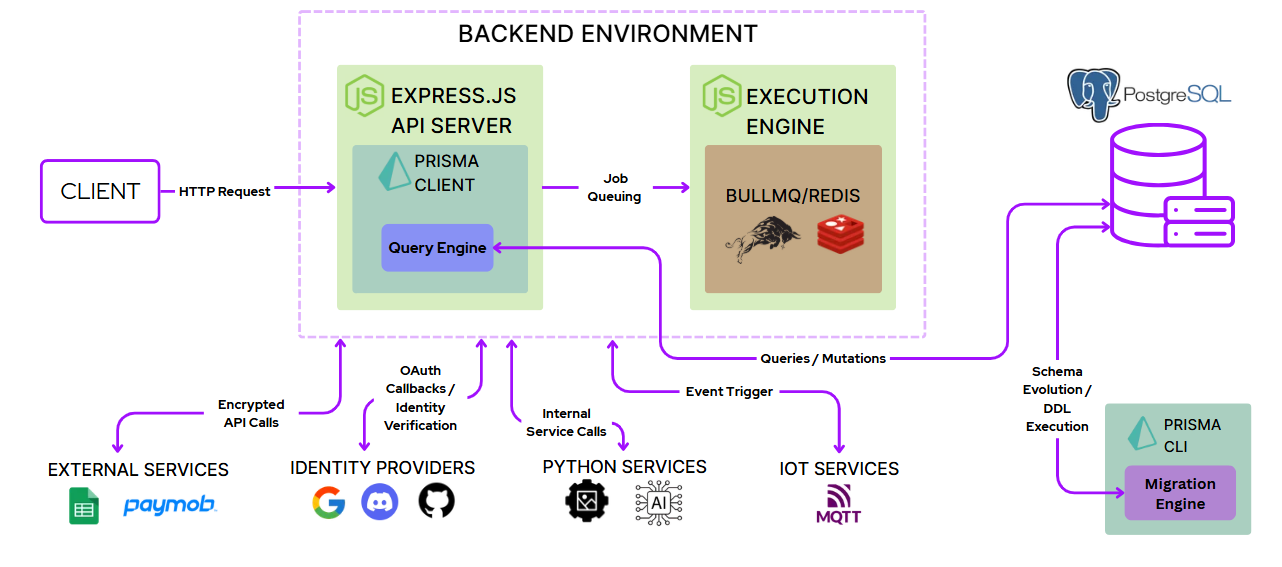
\includegraphics[width=\linewidth]{images/backend/backend_architecture_image.png}
    \caption{High-level Backend Architecture of the platform}
    \label{fig:backend-arch}
\end{figure}
\subsection{Request Lifecycle and Flow}

The lifecycle of a typical API request follows a strict sequential path designed to fail fast on invalid or unauthorized operations. The flow ensures that the core services and execution engine only ever process sanitized, authorized, and well-formed data. 
\begin{figure}[htbp]
\centering
\resizebox{\textwidth}{!}{
\begin{tikzpicture}[
  node distance=0.8cm and 2.5cm,
  box/.style={rectangle, draw=black, fill=blue!5, thick, minimum width=4.5cm, minimum height=1cm, text centered, rounded corners, font=\small},
  middleware/.style={rectangle, draw=black, fill=orange!10, thick, minimum width=4.5cm, minimum height=1cm, text centered, rounded corners, font=\small},
  logic/.style={rectangle, draw=black, fill=green!10, thick, minimum width=4.5cm, minimum height=1cm, text centered, rounded corners, font=\small},
  arrow/.style={thick, ->, >=stealth},
  dashed_arrow/.style={thick, ->, >=stealth, dashed}
]

% Main vertical pipeline
\node (client) [box, fill=gray!10] {Client Request};
\node (router) [box, below=of client] {API Router (\texttt{api.routes.ts})};
\node (rate) [middleware, below=of router] {Rate Limiter};
\node (auth) [middleware, below=of rate] {Auth \& RBAC Middlewares};
\node (validator) [middleware, below=of auth] {Request Validators};
\node (controller) [box, below=of validator] {Controller};
\node (service) [logic, below=of controller] {Service Layer};
\node (response) [box, fill=gray!10, below=of service] {JSend Response};

% Side nodes
\node (execution) [logic, left=of service] {Execution Engine};
\node (error) [middleware, fill=red!10, right=of validator] {Global Error Handler};

% Solid arrows (main flow)
\draw [arrow] (client) -- (router);
\draw [arrow] (router) -- (rate);
\draw [arrow] (rate) -- (auth);
\draw [arrow] (auth) -- (validator);
\draw [arrow] (validator) -- (controller);
\draw [arrow] (controller) -- (service);
\draw [arrow] (service) -- (response);
\draw [arrow] (service) -- (execution) node[midway, above, font=\scriptsize] {If required};

% Dashed arrows (Error handling) - routed cleanly to avoid overlapping
\draw [dashed_arrow] (auth.east) -| ([xshift=-0.5cm]error.north);
\draw [dashed_arrow] (validator.east) -- (error.west) node[midway, above, font=\scriptsize] {On failure};
\draw [dashed_arrow] (controller.east) -| ([xshift=-0.5cm]error.south);
\draw [dashed_arrow] (service.east) -| ([xshift=0.5cm]error.south);

\end{tikzpicture}
} % <--- Closed the resizebox here
\caption{High-level lifecycle of an incoming API request}
\label{fig:request-flow}
\end{figure}

\subsection{Backend System Layers}

The directory structure directly reflects the architectural boundaries of the application. Each layer has a single, distinct responsibility.

\subsubsection{Routes}
The routing layer is responsible for mapping incoming HTTP endpoints to their corresponding controller handlers. It acts as the entry point for the API hierarchy. Routes are logically grouped by entity (e.g., users, projects, workflows, nodes) and define the specific middleware chain required for each endpoint. 

By keeping the routing layer declarative, it provides a clear, high-level map of the entire API surface without bleeding into implementation details.

\subsubsection{Middlewares}
Middlewares act as the gatekeepers of the application. They intercept incoming requests to enforce systemic rules before the request can reach the business logic. This layer handles security concerns such as JSON Web Token (JWT) verification, role-based access control (RBAC), and email verification checks.

Additionally, middlewares manage traffic control via strict rate limiters, standardize outgoing success responses using the JSend format, and intercept exceptions through a centralized, registry-based error handling mechanism.

\subsubsection{Validators}
Request validation is abstracted into its own layer using \texttt{express-validator}. Before a request payload is processed, it is checked against strict schemas to ensure data integrity and type safety.

This layer ensures that bad payloads, missing parameters, or malformed data are rejected immediately with a \texttt{422 Unprocessable Entity} response. This "fail-fast" approach guarantees that the underlying controllers and services do not need to perform redundant sanity checks on incoming data.

\subsubsection{Controllers}
Controllers serve strictly as orchestrators between the HTTP transport layer and the business logic. A controller's only responsibility is to extract data from the incoming request (headers, body, params, query), pass that data to the appropriate service, and return the service's output back to the client.

Controllers are intentionally kept thin; they do not contain complex business rules or database queries, adhering strictly to the Single Responsibility Principle.

\subsubsection{Services}
The service layer forms the heart of the backend, encapsulating the core business logic of the FLOO platform. All heavy lifting—such as workflow graph construction, file processing with Cloudinary, communicating with the LLM via Groq, and interacting with the database—happens here.

By isolating business logic into services, the code becomes highly reusable and independently testable. For example, the execution engine can invoke a service method directly without needing to mock an HTTP request.

\subsubsection{Strategies}
The strategies layer encapsulates interchangeable authentication algorithms and behaviors, specifically leveraging Passport.js for OAuth 2.0 integrations. 

This directory contains the logic required to negotiate with external identity providers (such as Google, GitHub, and Discord) and third-party APIs like Google Sheets. Separating these into strategies allows the platform to easily scale the number of supported integrations without cluttering the core authentication flow.

\subsubsection{Utils}
The utils directory houses pure, stateless helper functions that are shared across multiple layers of the application. These include cryptographic operations like hashing passwords with \texttt{bcryptjs}, generating JWTs, and creating one-time passwords (OTPs) for email verification.

Because these functions are pure and self-contained, they are highly reliable and prevent code duplication throughout the codebase.

\paragraph{Cryptographic and Credential Utilities}
While many utilities handle standard platform tasks, the cryptographic helpers form the security backbone of the execution engine. These utilities bridge the gap between secure database storage and runtime execution.

\textbf{Encryption Engine (\texttt{encryption.util.ts}):}
All sensitive third-party secrets are encrypted at rest using the AES-256-CBC algorithm. The \texttt{encrypt} utility generates a unique 16-byte Initialization Vector (IV) for every operation, appending it to the resulting hexadecimal cipher to ensure maximum entropy. The corresponding \texttt{decrypt} function parses this combined string to extract the IV and securely reverse the operation, throwing a controlled application error if decryption fails.

\textbf{Credential Resolution (\texttt{credential.util.ts}):}
During workflow execution, nodes must access these secrets in plain text. The \texttt{getDecryptedCredentials} function acts as a secure bridge for the execution engine. When a node executes, this utility fetches the user's \texttt{UserCredentialSet} and its associated values from the database. 

It dynamically iterates through the requested parameters, checking the \texttt{isSensitive} metadata flag defined by the parameter schema. If a parameter is marked sensitive, it is routed through the decryption engine before being passed into the node's execution context; otherwise, it is returned as plain text. This guarantees that secrets remain securely encrypted in the database until the exact moment the execution engine requires them, while ensuring graceful failure logging if decryption encounters an error.

\subsubsection{Types}
TypeScript interfaces and type definitions form the foundational contract of the application. The types layer defines the exact shape of data structures used across the system, such as augmented Express Request objects (\texttt{AuthRequest}) or standardized OAuth profiles. 

This layer ensures strict compile-time safety, allowing the compiler to catch structural mismatches between the frontend payloads, the internal API representation, and the execution engine.





\section{Data Layer Architecture}

\subsection{Database Requirements}
The FLOO platform requires a robust, relational data storage layer capable of supporting multi-tenant isolation, complex configuration storage, and strict security compliance. The primary storage needs encompass:
\begin{itemize}
    \item \textbf{User and Identity Management:} Tracking local user profiles, multi-provider OAuth identities, and RBAC roles to ensure secure, isolated workspaces.
    \item \textbf{Project and Workflow Configurations:} Storing dynamic, graph-based automation logic and tracking deployment states.
    \item \textbf{Execution Analytics:} Persisting detailed logs of workflow runs, statuses, and generated outputs (such as Cloudinary asset links) for debugging and system analytics.
    \item \textbf{Secure Credential Management:} Safely storing third-party integration secrets (e.g., API keys, OAuth tokens) utilizing an encrypted, dynamically generated structure.
\end{itemize}

\textbf{Key Drivers:} Relational integrity is paramount due to the highly interconnected nature of the platform. For example, a User owns Projects, which trigger Executions, which in turn generate NodeOutputs. Transactional safety is explicitly required for operations like cascading account deletions, ensuring that scrubbing a user removes all associated relational assets without creating orphaned records. Prisma was selected as the ORM to enforce these strict foreign key constraints while providing end-to-end type safety with the TypeScript backend.

\subsection{Conceptual Design (ERD)}
The Conceptual Entity Relationship Diagram (CERD) outlines the high-level business entities and their interactions.

\begin{figure}[htbp]
    \centering
    \includegraphics[width=\linewidth,height=0.85\textheight,keepaspectratio]{images/erd/conceptual-erd.png}
    \caption{Conceptual Entity Relationship Diagram (CERD) for the FLOO platform}
    \label{fig:cerd}
\end{figure}

\subsubsection{Core Entity Relationships}
The conceptual model is heavily centered around the \texttt{User} entity, enforcing a strict ownership hierarchy:
\begin{itemize}
    \item \textbf{Users to Projects (1:N):} A single user can create and manage multiple automation projects. All workflow executions, chat histories, and node interactions branch off this fundamental relationship.
    \item \textbf{Projects to Executions (1:N):} Every time a workflow is triggered, an execution record is generated to track its lifecycle (e.g., NEW, RUNNING, SUCCESS, ERROR).
    \item \textbf{Nodes to Files (1:N):} External files are represented conceptually as inputs and outputs bound to specific execution instances and nodes, tracking cloud storage references.
\end{itemize}

\subsubsection{The Dynamic Credential Architecture}
A major architectural redesign was implemented in the credentials subsystem to provide a deep, highly flexible solution that seamlessly bridges backend storage with dynamic frontend UI rendering. 

Instead of hardcoding specific integration tokens into a single table, the system abstracts credentials into a definition-and-value pattern:
\begin{itemize}
    \item \textbf{Definition Phase:} Admins define a \texttt{CredentialType} (e.g., "Google Sheets" or "SMTP"). This type has a 1:N relationship with \texttt{CredentialParameterType}, which outlines the specific fields required (e.g., "API Key", "Client Secret").
    \item \textbf{UI Control Integration:} The \texttt{CredentialParameterType} includes metadata fields like \texttt{maxChar} and \texttt{isSensitive}. This design allows the frontend UI to automatically generate forms with appropriate validation and hidden password inputs without hardcoding frontend logic for every new integration type.
    \item \textbf{Value Phase:} When a user connects an integration, the system generates a \texttt{UserCredentialSet} linking to the \texttt{CredentialType}. The actual encrypted secrets are stored in \texttt{UserCredentialValue} records, creating a normalized mapping back to the expected parameters.
\end{itemize}

\subsection{Mapping to Relational Model (Logical/Physical Design)}
The logical design translates the conceptual entities into concrete database tables, explicitly defining keys, data types, and constraints utilizing the Prisma schema.

\begin{figure}[htbp]
    \centering
    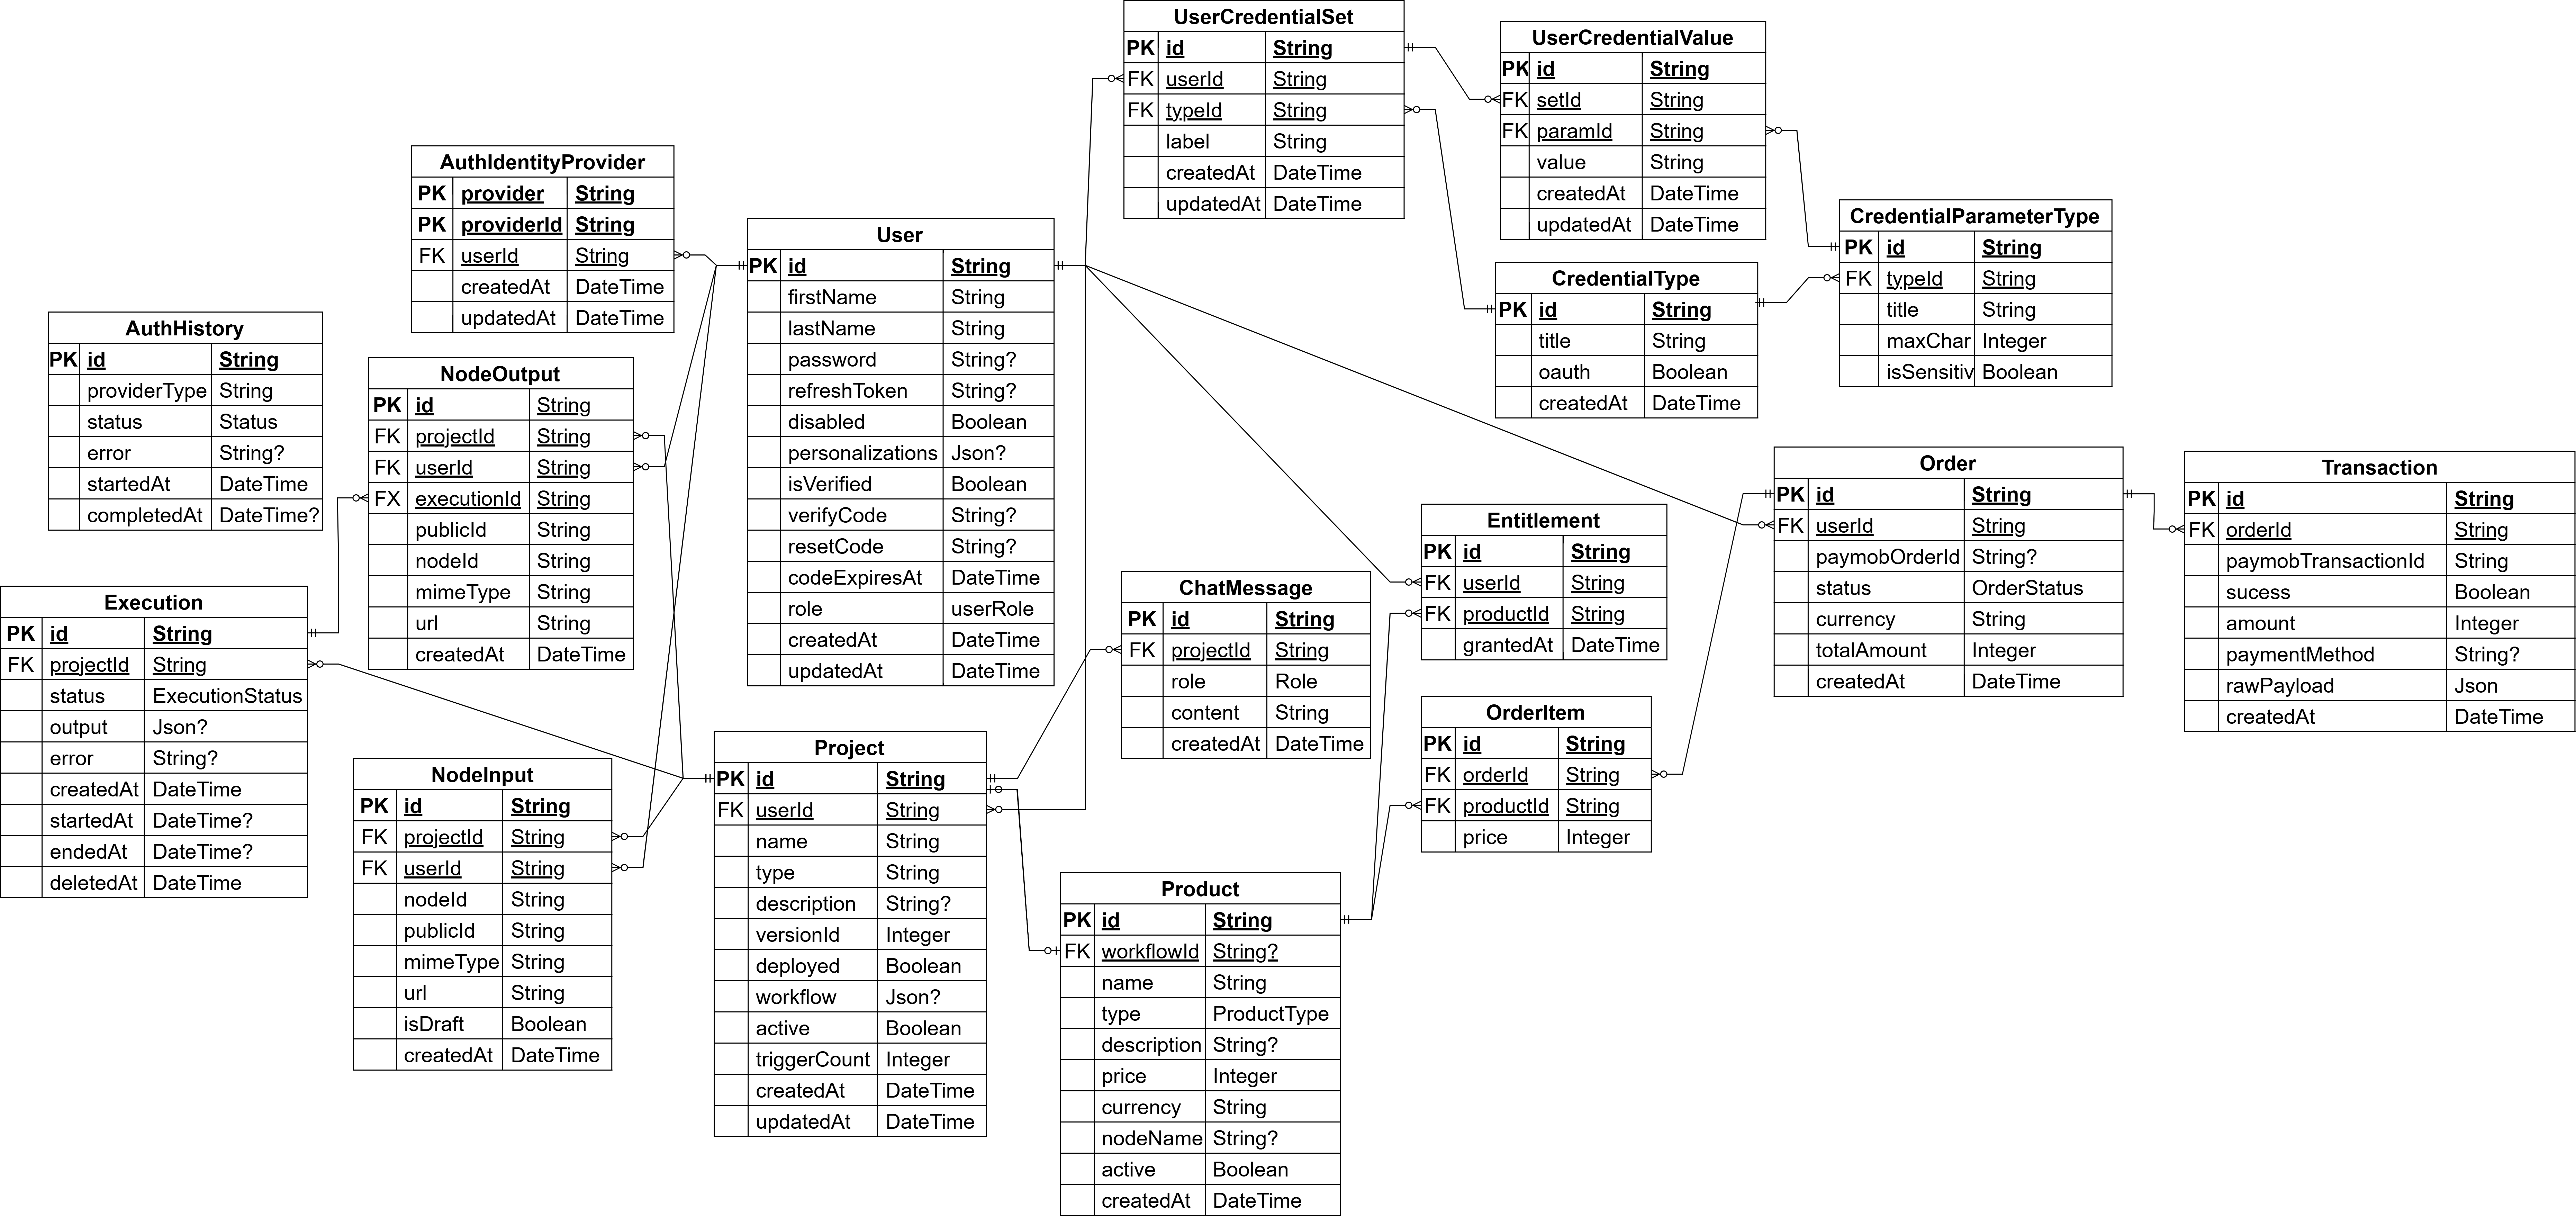
\includegraphics[width=0.95\linewidth,height=0.9\textheight,keepaspectratio]{images/erd/physical-erd.png}
    \captionof{figure}{Physical Entity Relationship Diagram (CERD) for the FLOO platform}
    \label{fig:perd}
\end{figure}

\subsubsection{Primary and Foreign Key Strategy}
\begin{itemize}
    \item \textbf{Universal UUIDs:} All primary keys (PK) across the platform utilize auto-generated UUIDs (e.g., \texttt{@id @default(uuid())}). This strategy prevents resource enumeration attacks and ensures global uniqueness, particularly useful when merging distributed data.
    \item \textbf{Composite Constraints:} Certain tables utilize composite keys to enforce logical uniqueness. For example, \texttt{\seqsplit{AuthIdentityProvider}} uses \texttt{\seqsplit{@@id([provider, providerId])}} to ensure a user cannot link the same third-party account twice. Similarly, \texttt{UserCredentialValue} enforces \texttt{\seqsplit{@@unique([setId, paramId])}} to guarantee only one value exists per parameter in a given credential set.
    \item \textbf{Aggressive Cascading Deletions:} To maintain strict data hygiene and comply with PII scrubbing requirements, foreign keys aggressively employ \texttt{onDelete: Cascade}. Deleting a User cascades down to erase their Projects, which in turn wipes Executions, Node Inputs, and Chat Messages instantly at the database level.
\end{itemize}

\subsubsection{Junction and Mapping Tables}
The database features specific mapping tables to resolve complex relationships. \texttt{\seqsplit{UserCredentialValue}} serves as the critical junction between a user's \texttt{\seqsplit{UserCredentialSet}} and the system's \texttt{\seqsplit{CredentialParameterType}}. This normalized approach ensures that if a parameter requirement changes at the system level, the relationship to the user's stored values remains structurally intact.

\subsubsection{Intentional Denormalization (JSON Workflows)}
While the database is heavily normalized, a deliberate exception was made for workflow graph configurations. Rather than splitting workflow nodes, edges, and positions into dozens of relational tables, the entire graph is serialized and stored in a \texttt{Json} column within the \texttt{Project} table (\texttt{workflow Json?}). 

This is a strategic design choice: workflow graphs are exclusively read and updated as a single atomic unit by the React Flow frontend. Normalizing the graph would require complex, expensive recursive SQL joins upon every canvas load. Utilizing a JSON column provides the necessary schema flexibility for varied node data while preserving high-performance read/write operations.

\subsection{Physical Database Architecture}

The physical database layer is implemented using PostgreSQL hosted on Supabase. We utilize Prisma ORM to enforce end-to-end type safety across the application. The schema is maintained through declarative migrations, ensuring that the database state is always synchronized with our TypeScript interfaces. Sensitive data, such as integration credentials, is stored using standard text fields, with robust encryption and decryption logic handled strictly at the Service Layer before ever reaching the persistence layer.

\subsubsection{Database Engine: PostgreSQL (via Supabase)}
PostgreSQL was selected as the underlying engine for its strict adherence to ACID compliance, robust support for relational integrity, and advanced JSON processing capabilities. Hosting via Supabase provides managed scaling, automated backups, and connection pooling, ensuring the database can handle high-frequency reads and writes typical of an automated workflow engine.

\subsubsection{ORM Layer (Prisma)}
Prisma acts as the bridge between the Node.js backend and the PostgreSQL database. Rather than writing raw SQL queries, the application relies on the generated Prisma Client.
\begin{itemize}
    \item \textbf{Type Safety:} The \texttt{schema.prisma} file serves as the single source of truth. Changes to the schema automatically regenerate TypeScript definitions, ensuring that any mismatched queries, missing fields, or incorrect data types are caught at compile-time rather than throwing unexpected runtime errors.
    \item \textbf{JSON Workflows:} Prisma natively supports PostgreSQL's \texttt{JSONB} data type, allowing the \texttt{Project} table to store complex, nested React Flow graphs in the \texttt{workflow} column without sacrificing query performance or requiring excessive normalization.
\end{itemize}

\subsubsection{Migration Management}
Database schema evolution is managed via Prisma Migrations. Instead of executing manual SQL scripts directly against production, developers modify the declarative Prisma schema. The migration engine then generates deterministic SQL differential scripts. This approach ensures that schema changes are strictly version-controlled, reproducible across local, staging, and production environments, and seamlessly integrated into the CI/CD pipeline.

\subsubsection{Technical Constraints}
To guarantee data integrity and query performance at scale, several constraints are baked directly into the physical schema:

\paragraph{Indexes}
Indexes are strategically applied to fields that are frequently used in `WHERE` clauses, sorting operations, or foreign key lookups to prevent full table scans:
\begin{itemize}
    \item \textbf{Foreign Key Lookups:} Indexes on \texttt{userId} within the \texttt{Project} and \texttt{NodeInput} tables drastically reduce query times when an authenticated user requests their dashboard.
    \item \textbf{Lookup Optimization:} The \texttt{email} column in the \texttt{User} table is indexed to optimize the high-frequency login and registration authentication flows.
    \item \textbf{Composite Indexes:} High-traffic logging tables utilize composite indexes, such as \texttt{@@index([executionId, nodeId])} on \texttt{NodeOutput}, enabling rapid retrieval of execution assets for the frontend analytics UI.
\end{itemize}

\paragraph{Constraints}
\begin{itemize}
    \item \textbf{Primary Keys:} All entities utilize UUIDs (\texttt{@id @default(uuid())}) as primary keys. This prevents resource enumeration attacks (e.g., guessing a user's ID) and facilitates distributed data merging.
    \item \textbf{Unique Constraints:} \texttt{@@unique} constraints enforce strict data uniqueness, such as ensuring no two users share an \texttt{email}, and no two files share a Cloudinary \texttt{publicId}.
    \item \textbf{Composite Uniques:} The \texttt{\seqsplit{UserCredentialValue}} table employs \texttt{\seqsplit{@@unique([setId, paramId])}} to guarantee that a specific credential set contains exactly one value per required parameter, preventing duplicate secret injection.
\end{itemize}

\paragraph{Cascade Rules \& Account Deletion}
Foreign key cascading is aggressively utilized to enforce data hygiene and simplify backend logic. In the schema, relations defining ownership are marked with \texttt{onDelete: Cascade}. 

This is highly crucial for the platform's \textbf{Account Deletion Flow}. When a user self-deletes (or is purged by an admin), the database engine natively and atomically destroys all linked \texttt{Project} rows. The cascade continues downward, automatically erasing all \texttt{Execution} logs, \texttt{NodeInput} assets, and \texttt{UserCredentialSet} secrets. This guarantees compliance with PII scrubbing requirements without requiring the application service layer to manually fetch and delete thousands of related rows, effectively preventing orphaned data.

\subsection{Data Dictionary}
The following tables detail the physical layout, constraints, and definitions of the core entities in the FLOO system, based on the finalized Prisma schema models.

\subsubsection{AuthHistory Table}
Tracks user authentication attempts and historical logs.
\begin{table}[H]
\centering
\renewcommand{\arraystretch}{1.3}
\begin{tabularx}{\textwidth}{|l|l|l|X|}
\hline
\textbf{Column Name} & \textbf{Type} & \textbf{Constraints} & \textbf{Description} \\
\hline
\texttt{id} & UUID & PK & Unique identifier for the log entry. \\
\hline
\texttt{providerType} & VARCHAR & Not Null & The type of authentication provider used. \\
\hline
\texttt{status} & ENUM & Default: ERROR & Status of the authentication (SUCCESS, ERROR). \\
\hline
\texttt{startedAt} & TIMESTAMP & Default: now() & When the authentication attempt started. \\
\hline
\texttt{completedAt} & TIMESTAMP & Nullable & When the authentication attempt finished. \\
\hline
\texttt{error} & TEXT & Nullable & Optional error message if the attempt failed. \\
\hline
\end{tabularx}
\caption{Data Dictionary: AuthHistory Table}
\label{tab:dict-authhistory}
\end{table}

\subsubsection{AuthIdentityProvider Table}
Links user accounts with external OAuth providers like Google or GitHub.
\begin{table}[H]
\centering
\renewcommand{\arraystretch}{1.3}
\begin{tabularx}{\textwidth}{|l|l|l|X|}
\hline
\textbf{Column Name} & \textbf{Type} & \textbf{Constraints} & \textbf{Description} \\
\hline
\texttt{userId} & UUID & FK, Cascade & References \texttt{User.id}. \\
\hline
\texttt{provider} & VARCHAR & PK (Composite) & Name of the identity provider. \\
\hline
\texttt{providerId} & VARCHAR & PK (Comp), Unique & Unique identifier from the provider. \\
\hline
\texttt{createdAt} & TIMESTAMP & Default: now() & Record creation time. \\
\hline
\texttt{updatedAt} & TIMESTAMP & Not Null & Auto-updating timestamp. \\
\hline
\end{tabularx}
\caption{Data Dictionary: AuthIdentityProvider Table}
\label{tab:dict-authidp}
\end{table}

\subsubsection{ChatMessage Table}
Stores interactions between users, the system, and the AI assistant within projects.
\begin{table}[H]
\centering
\renewcommand{\arraystretch}{1.3}
\begin{tabularx}{\textwidth}{|l|l|l|X|}
\hline
\textbf{Column Name} & \textbf{Type} & \textbf{Constraints} & \textbf{Description} \\
\hline
\texttt{id} & UUID & PK & Unique identifier for the message. \\
\hline
\texttt{projectId} & UUID & FK, Cascade, Index & References \texttt{Project.id}. Context of the chat. \\
\hline
\texttt{role} & ENUM & Not Null & Sender role (system, user, assistant). \\
\hline
\texttt{content} & TEXT & Not Null & The actual message content. \\
\hline
\texttt{createdAt} & TIMESTAMP & Default: now() & When the message was recorded. \\
\hline
\end{tabularx}
\caption{Data Dictionary: ChatMessage Table}
\label{tab:dict-chatmessage}
\end{table}

\subsubsection{CredentialParameterType Table}
Defines the individual fields required for a given credential type.
\begin{table}[H]
\centering
\renewcommand{\arraystretch}{1.3}
\begin{tabularx}{\textwidth}{|l|l|l|X|}
\hline
\textbf{Column Name} & \textbf{Type} & \textbf{Constraints} & \textbf{Description} \\
\hline
\texttt{id} & UUID & PK & Unique identifier for the parameter. \\
\hline
\texttt{typeId} & UUID & FK, Cascade & References \texttt{CredentialType.id}. \\
\hline
\texttt{title} & VARCHAR & Not Null & The name/label of the parameter. \\
\hline
\texttt{maxChar} & INT & Default: 2048 & Maximum length for tokens or encrypted strings. \\
\hline
\texttt{isSensitive} & BOOLEAN & Default: false & Flags whether the input should be hidden/encrypted. \\
\hline
\end{tabularx}
\caption{Data Dictionary: CredentialParameterType Table}
\label{tab:dict-credparamtype}
\end{table}

\subsubsection{CredentialType Table}
Declares global integration definitions (e.g., "Google Sheets", "SMTP").
\begin{table}[H]
\centering
\renewcommand{\arraystretch}{1.3}
\begin{tabularx}{\textwidth}{|l|l|l|X|}
\hline
\textbf{Column Name} & \textbf{Type} & \textbf{Constraints} & \textbf{Description} \\
\hline
\texttt{id} & UUID & PK & Unique identifier. \\
\hline
\texttt{title} & VARCHAR & Unique & The name of the integration type. \\
\hline
\texttt{oauth} & BOOLEAN & Default: false & Indicates if this type supports OAuth flow. \\
\hline
\texttt{createdAt} & TIMESTAMP & Default: now() & Record creation time. \\
\hline
\end{tabularx}
\caption{Data Dictionary: CredentialType Table}
\label{tab:dict-credtype}
\end{table}

\subsubsection{Entitlement Table}
Tracks permissions or access rights granted to users for specific products.
\begin{table}[H]
\centering
\renewcommand{\arraystretch}{1.3}
\begin{tabularx}{\textwidth}{|l|l|l|X|}
\hline
\textbf{Column Name} & \textbf{Type} & \textbf{Constraints} & \textbf{Description} \\
\hline
\texttt{id} & UUID & PK & Unique identifier. \\
\hline
\texttt{userId} & UUID & FK & References \texttt{User.id}. \\
\hline
\texttt{productId} & UUID & FK & References \texttt{Product.id}. \\
\hline
\texttt{grantedAt} & TIMESTAMP & Default: now() & When the entitlement was granted. \\
\hline
\end{tabularx}
\caption{Data Dictionary: Entitlement Table}
\label{tab:dict-entitlement}
\end{table}

\subsubsection{Execution Table}
Persists the lifecycle state and telemetry data for individual workflow runs.
\begin{table}[H]
\centering
\renewcommand{\arraystretch}{1.3}
\begin{tabularx}{\textwidth}{|l|l|l|X|}
\hline
\textbf{Column Name} & \textbf{Type} & \textbf{Constraints} & \textbf{Description} \\
\hline
\texttt{id} & UUID & PK & Unique tracking identifier for the job. \\
\hline
\texttt{projectId} & UUID & FK, Cascade & References \texttt{Project.id}. The triggered workflow. \\
\hline
\texttt{status} & ENUM & Default: NEW & Tracks current state (e.g., RUNNING, SUCCESS). \\
\hline
\texttt{output} & JSONB & Nullable & Stores general output details if available. \\
\hline
\texttt{createdAt} & TIMESTAMP & Default: now() & Record creation time. \\
\hline
\texttt{startedAt} & TIMESTAMP & Nullable & The exact time the execution picked up the job. \\
\hline
\texttt{endedAt} & TIMESTAMP & Nullable & Completion or crash time. \\
\hline
\texttt{deletedAt} & TIMESTAMP & Nullable & Tracks soft deletion state. \\
\hline
\texttt{error} & TEXT & Nullable & Execution stack traces or API failure messages. \\
\hline
\end{tabularx}
\caption{Data Dictionary: Execution Table}
\label{tab:dict-execution}
\end{table}

\subsubsection{NodeInput Table}
References external files and inputs provided to a node prior to execution.
\begin{table}[H]
\centering
\renewcommand{\arraystretch}{1.3}
\begin{tabularx}{\textwidth}{|l|l|l|X|}
\hline
\textbf{Column Name} & \textbf{Type} & \textbf{Constraints} & \textbf{Description} \\
\hline
\texttt{id} & UUID & PK & Unique identifier for the input file. \\
\hline
\texttt{nodeId} & VARCHAR & Index & Target node in the workflow. \\
\hline
\texttt{projectId} & UUID & FK, Cascade, Index & References \texttt{Project.id}. \\
\hline
\texttt{userId} & UUID & FK, Cascade, Index & References \texttt{User.id}. \\
\hline
\texttt{mimeType} & VARCHAR & Not Null & File content type. \\
\hline
\texttt{publicId} & VARCHAR & Unique & Provider ID (e.g., Cloudinary ID). \\
\hline
\texttt{url} & VARCHAR & Not Null & Direct access URL. \\
\hline
\texttt{isDraft} & BOOLEAN & Default: true & Determines if the input is pending commit. \\
\hline
\texttt{createdAt} & TIMESTAMP & Default: now() & Upload time. \\
\hline
\end{tabularx}
\caption{Data Dictionary: NodeInput Table}
\label{tab:dict-nodeinput}
\end{table}

\subsubsection{NodeOutput Table}
Tracks files and generated artifacts from nodes during a workflow execution.
\begin{table}[H]
\centering
\renewcommand{\arraystretch}{1.3}
\begin{tabularx}{\textwidth}{|l|l|l|X|}
\hline
\textbf{Column Name} & \textbf{Type} & \textbf{Constraints} & \textbf{Description} \\
\hline
\texttt{id} & UUID & PK & Unique identifier for the output file. \\
\hline
\texttt{nodeId} & VARCHAR & Index & Origin node in the workflow. \\
\hline
\texttt{executionId} & UUID & FK, Cascade, Index & References \texttt{Execution.id}. \\
\hline
\texttt{projectId} & UUID & FK, Cascade, Index & References \texttt{Project.id}. \\
\hline
\texttt{userId} & UUID & FK, Cascade, Index & References \texttt{User.id}. \\
\hline
\texttt{mimeType} & VARCHAR & Not Null & File content type. \\
\hline
\texttt{publicId} & VARCHAR & Unique & Provider ID (e.g., Cloudinary ID). \\
\hline
\texttt{url} & VARCHAR & Not Null & Direct access URL. \\
\hline
\texttt{createdAt} & TIMESTAMP & Default: now() & Generation time. \\
\hline
\end{tabularx}
\caption{Data Dictionary: NodeOutput Table}
\label{tab:dict-nodeoutput}
\end{table}

\subsubsection{Order Table}
Tracks user purchases and financial operations on the platform.
\begin{table}[H]
\centering
\renewcommand{\arraystretch}{1.3}
\begin{tabularx}{\textwidth}{|l|l|l|X|}
\hline
\textbf{Column Name} & \textbf{Type} & \textbf{Constraints} & \textbf{Description} \\
\hline
\texttt{id} & UUID & PK & Unique identifier. \\
\hline
\texttt{userId} & UUID & FK & References \texttt{User.id}. \\
\hline
\texttt{paymobOrderId} & VARCHAR & Unique, Nullable & External reference to the payment gateway order. \\
\hline
\texttt{totalAmount} & INT & Not Null & Value in cents. \\
\hline
\texttt{currency} & VARCHAR & Default: "EGP" & Currency of the transaction. \\
\hline
\texttt{status} & ENUM & Default: PENDING & Current status (PENDING, PAID, FAILED). \\
\hline
\texttt{createdAt} & TIMESTAMP & Default: now() & When the order was created. \\
\hline
\end{tabularx}
\caption{Data Dictionary: Order Table}
\label{tab:dict-order}
\end{table}

\subsubsection{OrderItem Table}
Associates individual products with an order.
\begin{table}[H]
\centering
\renewcommand{\arraystretch}{1.3}
\begin{tabularx}{\textwidth}{|l|l|l|X|}
\hline
\textbf{Column Name} & \textbf{Type} & \textbf{Constraints} & \textbf{Description} \\
\hline
\texttt{id} & UUID & PK & Unique identifier. \\
\hline
\texttt{orderId} & UUID & FK, Cascade & References \texttt{Order.id}. \\
\hline
\texttt{productId} & UUID & FK & References \texttt{Product.id}. \\
\hline
\texttt{price} & INT & Not Null & Price in cents at time of order. \\
\hline
\end{tabularx}
\caption{Data Dictionary: OrderItem Table}
\label{tab:dict-orderitem}
\end{table}

\subsubsection{Product Table}
Defines templates or node expansions available on the platform.
\begin{table}[H]
\centering
\renewcommand{\arraystretch}{1.3}
\begin{tabularx}{\textwidth}{|l|l|l|X|}
\hline
\textbf{Column Name} & \textbf{Type} & \textbf{Constraints} & \textbf{Description} \\
\hline
\texttt{id} & UUID & PK & Unique identifier. \\
\hline
\texttt{name} & VARCHAR & Not Null & Product name. \\
\hline
\texttt{type} & ENUM & Not Null & Type classification (TEMPLATE or NODE). \\
\hline
\texttt{workflowId} & UUID & FK, Unique, Nullable & References \texttt{Project.id} if it's a template. \\
\hline
\texttt{nodeName} & VARCHAR & Unique, Nullable & Associated node identifier. \\
\hline
\texttt{price} & INT & Not Null & Price in cents. \\
\hline
\texttt{currency} & VARCHAR & Default: "EGP" & Currency. \\
\hline
\texttt{description} & TEXT & Nullable & Information about the product. \\
\hline
\texttt{createdAt} & TIMESTAMP & Default: now() & Creation time. \\
\hline
\texttt{active} & BOOLEAN & Default: true & Whether it's actively available for purchase. \\
\hline
\end{tabularx}
\caption{Data Dictionary: Product Table}
\label{tab:dict-product}
\end{table}

\subsubsection{Project Table}
Stores the configuration and state of the user's workflow automations.
\begin{table}[H]
\centering
\renewcommand{\arraystretch}{1.3}
\begin{tabularx}{\textwidth}{|l|l|l|X|}
\hline
\textbf{Column Name} & \textbf{Type} & \textbf{Constraints} & \textbf{Description} \\
\hline
\texttt{id} & UUID & PK & Unique identifier for the project. \\
\hline
\texttt{name} & VARCHAR & Not Null & Human-readable name of the automation. \\
\hline
\texttt{type} & VARCHAR & Not Null & Category or type of project. \\
\hline
\texttt{description} & TEXT & Nullable & Optional details about the automation logic. \\
\hline
\texttt{createdAt} & TIMESTAMP & Default: now() & When the project was generated. \\
\hline
\texttt{updatedAt} & TIMESTAMP & Not Null & Auto-updating timestamp. \\
\hline
\texttt{deployed} & BOOLEAN & Default: false & Tracks whether the project is actively running. \\
\hline
\texttt{versionId} & INT & Default: 1 & Tracks revisions made to the workflow logic. \\
\hline
\texttt{workflow} & JSONB & Nullable & Serialized React Flow graph containing node definitions. \\
\hline
\texttt{active} & BOOLEAN & Default: true & General availability state of the project. \\
\hline
\texttt{triggerCount} & INT & Default: 0 & Aggregate count of triggers handled by the project. \\
\hline
\texttt{userId} & UUID & FK, Cascade & References \texttt{User.id}. Defines ownership. \\
\hline
\end{tabularx}
\caption{Data Dictionary: Project Table}
\label{tab:dict-project}
\end{table}

\subsubsection{Transaction Table}
Records individual payment gateway transactions for auditability.
\begin{table}[H]
\centering
\renewcommand{\arraystretch}{1.3}
\begin{tabularx}{\textwidth}{|l|l|l|X|}
\hline
\textbf{Column Name} & \textbf{Type} & \textbf{Constraints} & \textbf{Description} \\
\hline
\texttt{id} & UUID & PK & Unique identifier. \\
\hline
\texttt{orderId} & UUID & FK & References \texttt{Order.id}. \\
\hline
\texttt{paymobTransactionId} & VARCHAR & Unique & Associated remote ID from Paymob Webhook. \\
\hline
\texttt{success} & BOOLEAN & Not Null & If the remote transaction cleared successfully. \\
\hline
\texttt{amount} & INT & Not Null & Processed amount in cents. \\
\hline
\texttt{paymentMethod} & VARCHAR & Nullable & 'card', 'wallet', etc. \\
\hline
\texttt{rawPayload} & JSONB & Not Null & Complete provider payload for debugging. \\
\hline
\texttt{createdAt} & TIMESTAMP & Default: now() & Event timestamp. \\
\hline
\end{tabularx}
\caption{Data Dictionary: Transaction Table}
\label{tab:dict-transaction}
\end{table}

\subsubsection{User Table}
Serves as the root entity for identity, access control, and ownership.
\begin{table}[H]
\centering
\renewcommand{\arraystretch}{1.3}
\begin{tabularx}{\textwidth}{|l|l|l|X|}
\hline
\textbf{Column Name} & \textbf{Type} & \textbf{Constraints} & \textbf{Description} \\
\hline
\texttt{id} & UUID & PK & Unique identifier for the user. \\
\hline
\texttt{email} & VARCHAR & Unique, Index & The user's primary email address for authentication. \\
\hline
\texttt{firstName} & VARCHAR & Not Null & The user's first name. \\
\hline
\texttt{lastName} & VARCHAR & Not Null & The user's last name. \\
\hline
\texttt{password} & VARCHAR & Nullable & Bcrypt-hashed local password. Null if strictly OAuth. \\
\hline
\texttt{refreshToken} & VARCHAR & Nullable & Active JWT refresh token for maintaining sessions. \\
\hline
\texttt{disabled} & BOOLEAN & Default: false & Soft-deletion and ban tracker. \\
\hline
\texttt{personalizations} & JSONB & Nullable & Custom UI/UX preferences payload. \\
\hline
\texttt{isVerified} & BOOLEAN & Default: false & Gates access to execution features until email is confirmed. \\
\hline
\texttt{verifyCode} & VARCHAR & Nullable & The active OTP code for email verification. \\
\hline
\texttt{resetCode} & VARCHAR & Nullable & The active OTP code for password resets. \\
\hline
\texttt{codeExpiresAt} & TIMESTAMP & Nullable & Time limit to act upon the verify/reset codes. \\
\hline
\texttt{role} & ENUM & Default: USER & Defines RBAC privileges (USER or ADMIN). \\
\hline
\texttt{createdAt} & TIMESTAMP & Default: now() & Timestamp of account registration. \\
\hline
\texttt{updatedAt} & TIMESTAMP & Not Null & Auto-updating timestamp. \\
\hline
\end{tabularx}
\caption{Data Dictionary: User Table}
\label{tab:dict-user}
\end{table}

\subsubsection{UserCredentialSet Table}
Acts as the parent entity for a group of encrypted third-party integration secrets.
\begin{table}[H]
\centering
\renewcommand{\arraystretch}{1.3}
\begin{tabularx}{\textwidth}{|l|l|l|X|}
\hline
\textbf{Column Name} & \textbf{Type} & \textbf{Constraints} & \textbf{Description} \\
\hline
\texttt{id} & UUID & PK & Unique identifier for the credential set. \\
\hline
\texttt{userId} & UUID & FK, Cascade & References \texttt{User.id}. Determines who can use these credentials. \\
\hline
\texttt{typeId} & UUID & FK, Cascade & References \texttt{CredentialType.id} (e.g., Google Sheets, SMTP). \\
\hline
\texttt{label} & VARCHAR & Not Null & User-defined alias for the credentials (e.g., "My Work Gmail"). \\
\hline
\texttt{createdAt} & TIMESTAMP & Default: now() & Time of creation. \\
\hline
\texttt{updatedAt} & TIMESTAMP & Not Null & Auto-updating timestamp. \\
\hline
\end{tabularx}
\caption{Data Dictionary: UserCredentialSet Table}
\label{tab:dict-credentialset}
\end{table}

\subsubsection{UserCredentialValue Table}
Stores the actual encrypted parameters required by a credential set.
\begin{table}[H]
\centering
\renewcommand{\arraystretch}{1.3}
\begin{tabularx}{\textwidth}{|l|l|l|X|}
\hline
\textbf{Column Name} & \textbf{Type} & \textbf{Constraints} & \textbf{Description} \\
\hline
\texttt{id} & UUID & PK & Unique identifier. \\
\hline
\texttt{setId} & UUID & FK, Cascade & References \texttt{UserCredentialSet.id}. \\
\hline
\texttt{paramId} & UUID & FK, Cascade & References \texttt{CredentialParameterType.id}. \\
\hline
\texttt{value} & TEXT & Not Null & The securely encrypted string containing the secret. \\
\hline
\texttt{createdAt} & TIMESTAMP & Default: now() & Creation time. \\
\hline
\texttt{updatedAt} & TIMESTAMP & Not Null & Auto-updating timestamp. \\
\hline
\end{tabularx}
\caption{Data Dictionary: UserCredentialValue Table}
\label{tab:dict-credentialvalue}
\end{table}





\section{API Design and Functional Flows}
\subsection{API Overview}

The FLOO platform is built on a modular, multi-layered architecture using Node.js, Express.js, and TypeScript, designed to ensure a strict separation of concerns between routing, business logic, security, and execution.

\subsubsection{RESTful Conventions}
The API is designed around RESTful principles, where resources are mapped to intuitive endpoints categorized by entity (e.g., \texttt{/user}, \texttt{/project}, \texttt{/node}, \texttt{/credential}). By maintaining a declarative routing structure, the API surface remains clean and self-documenting, preventing business logic from bleeding into the transport layer. The platform utilizes standard HTTP verbs to perform operations:
\begin{itemize}
    \item \textbf{GET}: Retrieve data or list resources.
    \item \textbf{POST}: Create new resources or trigger actions.
    \item \textbf{PATCH}: Update existing resource metadata.
    \item \textbf{DELETE}: Remove specific resources or clear session data.
\end{itemize}

\subsubsection{Authentication and Security}
Security is enforced through a tiered middleware system that acts as the application's gatekeeper.
\begin{itemize}
    \item \textbf{JWT Authentication}: Most endpoints require a valid JSON Web Token (JWT) processed by the \texttt{auth} middleware to identify the requesting user.
    \item \textbf{Role-Based Access Control (RBAC)}: Sensitive routes utilize the \texttt{restrictTo} middleware to enforce fine-grained access based on user roles (\texttt{USER} vs \texttt{ADMIN}).
    \item \textbf{Verification Gate}: Critical operations, such as managing projects or executing workflows, are protected by the \texttt{restrictToVerified} middleware, ensuring only accounts with confirmed emails can perform these actions.
    \item \textbf{Public Access}: Certain endpoints, such as initial Auth/OAuth routes and Webhook triggers, allow public access. These are not left unprotected but are instead secured via dedicated, high-threshold rate limiters.
\end{itemize}

\subsubsection{Response Format and Standardization}
To ensure consistency across the platform, all responses adhere to the \textbf{JSend} format, providing a predictable structure for the frontend.

\paragraph{HTTP Status Codes}
The API utilizes standard HTTP status codes to communicate outcome states:
\begin{table}[H]
\centering
\begin{tabular}{|l|p{8cm}|}
\hline
\textbf{Code} & \textbf{Meaning} \\
\hline
\texttt{200/201} & Successful request or creation. \\
\hline
\texttt{400} & Bad Request (Missing fields, validation failure). \\
\hline
\texttt{401} & Authentication failed (Expired or invalid token). \\
\hline
\texttt{403} & Forbidden (Insufficient permissions or unverified email). \\
\hline
\texttt{404} & Resource not found. \\
\hline
\texttt{429} & Too Many Requests (Rate limit exceeded). \\
\hline
\texttt{500} & Internal Server Error (Unexpected system failure). \\
\hline
\end{tabular}
\end{table}

\paragraph{Rate Limiting}
Traffic control is central to platform stability. The system employs multiple tiers of rate limiting:
\begin{itemize}
    \item \textbf{Standard Limit}: Most API routes are subject to a global limit of 150 requests per 15 minutes to prevent abuse.
    \item \textbf{Action-Specific Limits}: Critical actions have stricter, dedicated limits—such as manual workflow execution (30/min), file uploads (20/15min), or OAuth requests (10/15min)—to protect high-cost resources.
    \item \textbf{Public Limits}: High-volume triggers, like webhooks, utilize a loose limit (e.g., 1000/min) to accommodate frequent event spikes from external providers.
\end{itemize}

\subsection{Endpoints Reference}
\subsubsection{Auth Endpoints}
\label{subsec:auth-endpoints}

This section documents all API endpoints related to user authentication, registration, and session management in FLOO. Most of these endpoints are public but are protected by strict rate limiters and payload validators (\texttt{validateRequest}) to ensure security and prevent abuse.

% ─────────────────────────────────────────────
\paragraph{Register User}
\label{subsubsec:register-user}

\begin{itemize}
  \item \textbf{Endpoint:} \texttt{POST /api/auth/register}
  \item \textbf{Access:} \texttt{PUBLIC}
  \item \textbf{Description:} Creates a new user account and sends a verification code (OTP) to the provided email. Rate limited to 3 requests per hour per IP.
\end{itemize}

\begin{table}[H]
\centering
\renewcommand{\arraystretch}{1.3}
\begin{tabularx}{\textwidth}{|l|l|l|X|}
\hline
\textbf{Field} & \textbf{Location} & \textbf{Type} & \textbf{Description} \\
\hline
\texttt{email}     & Body & \texttt{string} & \textbf{Required.} User's email address \\
\hline
\texttt{password}  & Body & \texttt{string} & \textbf{Required.} User's password \\
\hline
\texttt{firstName} & Body & \texttt{string} & \textbf{Required.} User's first name \\
\hline
\texttt{lastName}  & Body & \texttt{string} & \textbf{Required.} User's last name \\
\hline
\end{tabularx}
\caption{POST /api/auth/register — Request Body}
\label{tab:register-body}
\end{table}

\begin{table}[H]
\centering
\renewcommand{\arraystretch}{1.3}
\begin{tabularx}{\textwidth}{|l|l|X|}
\hline
\textbf{Status Code} & \textbf{Condition} & \textbf{Description} \\
\hline
\texttt{201 Created}      & Success            & Verification code sent, returns user and tokens \\
\hline
\texttt{409 Conflict}     & Email in use       & A user with this email already exists \\
\hline
\texttt{422 Unprocessable Entity} & Validation failed & Required fields missing or invalid \\
\hline
\texttt{429 Too Many Requests} & Rate limit exceeded & Too many accounts created from this IP, please try again after an hour \\
\hline
\texttt{500 Internal Server Error} & Server error & Unexpected failure or email delivery issue \\
\hline
\end{tabularx}
\caption{POST /api/auth/register — Response Codes}
\label{tab:register-responses}
\end{table}
\FloatBarrier

% ─────────────────────────────────────────────
\paragraph{Login User}
\label{subsubsec:login-user}

\begin{itemize}
  \item \textbf{Endpoint:} \texttt{POST /api/auth/login}
  \item \textbf{Access:} \texttt{PUBLIC}
  \item \textbf{Description:} Authenticates a user using email and password. Cannot be used for accounts created exclusively via OAuth. Rate limited to 5 attempts per 15 minutes per IP.
\end{itemize}

\begin{table}[H]
\centering
\renewcommand{\arraystretch}{1.3}
\begin{tabularx}{\textwidth}{|l|l|l|X|}
\hline
\textbf{Field} & \textbf{Location} & \textbf{Type} & \textbf{Description} \\
\hline
\texttt{email}    & Body & \texttt{string} & \textbf{Required.} The user's email \\
\hline
\texttt{password} & Body & \texttt{string} & \textbf{Required.} The user's password \\
\hline
\end{tabularx}
\caption{POST /api/auth/login — Request Body}
\label{tab:login-body}
\end{table}

\begin{table}[H]
\centering
\renewcommand{\arraystretch}{1.3}
\begin{tabularx}{\textwidth}{|l|l|X|}
\hline
\textbf{Status Code} & \textbf{Condition} & \textbf{Description} \\
\hline
\texttt{200 OK}           & Success            & Returns user data, access token, and refresh token \\
\hline
\texttt{401 Unauthorized} & Invalid credentials & Wrong email, password, or OAuth-only account \\
\hline
\texttt{422 Unprocessable Entity} & Validation failed & Required fields missing or invalid \\
\hline
\texttt{429 Too Many Requests} & Rate limit exceeded & Too many login attempts from this IP, please try again after 15 minutes \\
\hline
\texttt{500 Internal Server Error} & Server error & Unexpected failure \\
\hline
\end{tabularx}
\caption{POST /api/auth/login — Response Codes}
\label{tab:login-responses}
\end{table}
\FloatBarrier

% ─────────────────────────────────────────────
\paragraph{Forgot Password}
\label{subsubsec:forgot-password}

\begin{itemize}
  \item \textbf{Endpoint:} \texttt{POST /api/auth/forgot-password}
  \item \textbf{Access:} \texttt{PUBLIC}
  \item \textbf{Description:} Generates a 15-minute OTP and sends it to the user's email to reset their password. Always returns a success message for security reasons, even if the email is unregistered. Rate limited to 3 requests per hour.
\end{itemize}

\begin{table}[H]
\centering
\renewcommand{\arraystretch}{1.3}
\begin{tabularx}{\textwidth}{|l|l|l|X|}
\hline
\textbf{Field} & \textbf{Location} & \textbf{Type} & \textbf{Description} \\
\hline
\texttt{email} & Body & \texttt{string} & \textbf{Required.} The account email address \\
\hline
\end{tabularx}
\caption{POST /api/auth/forgot-password — Request Body}
\label{tab:forgot-password-body}
\end{table}

\begin{table}[H]
\centering
\renewcommand{\arraystretch}{1.3}
\begin{tabularx}{\textwidth}{|l|l|X|}
\hline
\textbf{Status Code} & \textbf{Condition} & \textbf{Description} \\
\hline
\texttt{200 OK}           & Success            & Reset code sent successfully \\
\hline
\texttt{422 Unprocessable Entity} & Validation failed & Invalid email format \\
\hline
\texttt{429 Too Many Requests} & Rate limit exceeded & Too many password reset requests, please try again after an hour \\
\hline
\texttt{500 Internal Server Error} & Server error & Unexpected failure or email delivery issue \\
\hline
\end{tabularx}
\caption{POST /api/auth/forgot-password — Response Codes}
\label{tab:forgot-password-responses}
\end{table}
\FloatBarrier

% ─────────────────────────────────────────────
\paragraph{Verify Reset Code (Reset Password)}
\label{subsubsec:reset-password}

\begin{itemize}
  \item \textbf{Endpoint:} \texttt{POST /api/auth/reset-password}
  \item \textbf{Access:} \texttt{PUBLIC}
  \item \textbf{Description:} Validates the OTP sent via email and updates the user's password. The new password cannot match the old password. Rate limited to 3 requests per hour.
\end{itemize}

\begin{table}[H]
\centering
\renewcommand{\arraystretch}{1.3}
\begin{tabularx}{\textwidth}{|l|l|l|X|}
\hline
\textbf{Field} & \textbf{Location} & \textbf{Type} & \textbf{Description} \\
\hline
\texttt{email}     & Body & \texttt{string} & \textbf{Required.} The account email \\
\hline
\texttt{resetCode} & Body & \texttt{string} & \textbf{Required.} The OTP sent to the user \\
\hline
\texttt{password}  & Body & \texttt{string} & \textbf{Required.} The new password \\
\hline
\end{tabularx}
\caption{POST /api/auth/reset-password — Request Body}
\label{tab:reset-password-body}
\end{table}

\begin{table}[H]
\centering
\renewcommand{\arraystretch}{1.3}
\begin{tabularx}{\textwidth}{|l|l|X|}
\hline
\textbf{Status Code} & \textbf{Condition} & \textbf{Description} \\
\hline
\texttt{200 OK}           & Success             & Password reset successfully \\
\hline
\texttt{400 Bad Request}  & Invalid code        & The OTP is incorrect or expired \\
\hline
\texttt{401 Unauthorized} & Same password       & The new password is the same as the old one \\
\hline
\texttt{422 Unprocessable Entity} & Validation failed & Missing fields or invalid format \\
\hline
\texttt{429 Too Many Requests} & Rate limit exceeded & Too many password reset requests, please try again after an hour \\
\hline
\texttt{500 Internal Server Error} & Server error & Unexpected failure \\
\hline
\end{tabularx}
\caption{POST /api/auth/reset-password — Response Codes}
\label{tab:reset-password-responses}
\end{table}
\FloatBarrier

% ─────────────────────────────────────────────
\paragraph{Refresh Token}
\label{subsubsec:refresh-token}

\begin{itemize}
  \item \textbf{Endpoint:} \texttt{POST /api/auth/refresh-token}
  \item \textbf{Access:} \texttt{PUBLIC}
  \item \textbf{Description:} Exchanges a valid refresh token for a new access token. Validates against the hashed token stored in the database. Rate limited to 5 requests per 15 minutes.
\end{itemize}

\begin{table}[H]
\centering
\renewcommand{\arraystretch}{1.3}
\begin{tabularx}{\textwidth}{|l|l|l|X|}
\hline
\textbf{Field} & \textbf{Location} & \textbf{Type} & \textbf{Description} \\
\hline
\texttt{refreshToken} & Body & \texttt{string} & \textbf{Required.} The user's active refresh token \\
\hline
\end{tabularx}
\caption{POST /api/auth/refresh-token — Request Body}
\label{tab:refresh-token-body}
\end{table}

\begin{table}[H]
\centering
\renewcommand{\arraystretch}{1.3}
\begin{tabularx}{\textwidth}{|l|l|X|}
\hline
\textbf{Status Code} & \textbf{Condition} & \textbf{Description} \\
\hline
\texttt{200 OK}           & Success              & Returns a new access token \\
\hline
\texttt{401 Unauthorized} & Invalid token        & Token is expired, missing in DB, or invalid \\
\hline
\texttt{429 Too Many Requests} & Rate limit exceeded & Too many token refresh requests from this IP \\
\hline
\texttt{500 Internal Server Error} & Server error & Unexpected failure \\
\hline
\end{tabularx}
\caption{POST /api/auth/refresh-token — Response Codes}
\label{tab:refresh-token-responses}
\end{table}
\FloatBarrier

% ─────────────────────────────────────────────
\paragraph{OAuth Initiation}
\label{subsubsec:oauth-initiation}

\begin{itemize}
  \item \textbf{Endpoints:} 
  \texttt{\seqsplit{GET /api/auth/discord}}, 
  \texttt{\seqsplit{GET /api/auth/google}}, 
  \texttt{\seqsplit{GET /api/auth/github}}
  \item \textbf{Access:} \texttt{\seqsplit{PUBLIC}}
  \item \textbf{Description:} Initiates the OAuth flow by redirecting the user to the respective provider's authentication page. Supports dynamic redirect configuration based on the client type. Rate limited to 10 requests per 15 minutes.
\end{itemize}

\begin{table}[H]
\centering
\renewcommand{\arraystretch}{1.3}
\begin{tabularx}{\textwidth}{|l|l|l|X|}
\hline
\textbf{Parameter} & \textbf{Location} & \textbf{Type} & \textbf{Description} \\
\hline
\texttt{client}    & Query & \texttt{string} & Optional. Pass \texttt{flutter} for mobile deep linking \\
\hline
\end{tabularx}
\caption{GET /api/auth/\{provider\} — Query Parameters}
\label{tab:oauth-initiation-params}
\end{table}

% ─────────────────────────────────────────────
\paragraph{OAuth Callback}
\label{subsubsec:oauth-callback}

\begin{itemize}
  \item \textbf{Endpoints:} 
  \texttt{\seqsplit{GET /api/auth/discord/callback}}, 
  \texttt{\seqsplit{GET /api/auth/google/callback}}, 
  \texttt{\seqsplit{GET /api/auth/github/callback}}
  \item \textbf{Access:} \texttt{\seqsplit{PUBLIC}}
  \item \textbf{Description:} Handled by Passport.js strategies. Upon successful authentication, it generates a secure 15-second ticket stored in Redis and redirects to the client application (Web or Flutter) with the ticket appended as a query parameter. Rate limited to 10 requests per 15 minutes.
\end{itemize}

\begin{table}[H]
\centering
\renewcommand{\arraystretch}{1.3}
\begin{tabularx}{\textwidth}{|l|l|X|}
\hline
\textbf{Status Code} & \textbf{Condition} & \textbf{Description} \\
\hline
\texttt{302 Found}        & Success            & Redirects to client URL with \texttt{?ticket=UUID} \\
\hline
\texttt{401 Unauthorized} & Auth failed        & Failed to login with the OAuth provider \\
\hline
\texttt{429 Too Many Requests} & Rate limit exceeded & Too many OAuth requests \\
\hline
\texttt{500 Internal Server Error} & Server error & Unexpected failure \\
\hline
\end{tabularx}
\caption{GET /api/auth/\{provider\}/callback — Response Codes}
\label{tab:oauth-callback-responses}
\end{table}
\FloatBarrier

% ─────────────────────────────────────────────
\paragraph{Exchange Ticket}
\label{subsubsec:exchange-ticket}

\begin{itemize}
  \item \textbf{Endpoint:} \texttt{POST /api/auth/exchange}
  \item \textbf{Access:} \texttt{PUBLIC}
  \item \textbf{Description:} Exchanges the temporary Redis ticket obtained from the OAuth callback for the actual user data, access token, and refresh token. The ticket is single-use and expires in 15 seconds. Rate limited to 10 requests per 15 minutes.
\end{itemize}

\begin{table}[H]
\centering
\renewcommand{\arraystretch}{1.3}
\begin{tabularx}{\textwidth}{|l|l|l|X|}
\hline
\textbf{Field} & \textbf{Location} & \textbf{Type} & \textbf{Description} \\
\hline
\texttt{ticket} & Body & \texttt{string} & \textbf{Required.} The UUID ticket from the OAuth redirect \\
\hline
\end{tabularx}
\caption{POST /api/auth/exchange — Request Body}
\label{tab:exchange-ticket-body}
\end{table}

\begin{table}[H]
\centering
\renewcommand{\arraystretch}{1.3}
\begin{tabularx}{\textwidth}{|l|l|X|}
\hline
\textbf{Status Code} & \textbf{Condition} & \textbf{Description} \\
\hline
\texttt{200 OK}           & Success              & Ticket exchanged, returns user and tokens \\
\hline
\texttt{400 Bad Request}  & Invalid ticket       & The ticket is invalid, expired, or already used \\
\hline
\texttt{422 Unprocessable Entity} & Validation failed & Missing ticket in request body \\
\hline
\texttt{429 Too Many Requests} & Rate limit exceeded & Too many OAuth requests \\
\hline
\texttt{500 Internal Server Error} & Server error & Unexpected failure \\
\hline
\end{tabularx}
\caption{POST /api/auth/exchange — Response Codes}
\label{tab:exchange-ticket-responses}
\end{table}
\FloatBarrier
\subsubsection{User Endpoints}
\label{subsec:user-endpoints}

This section documents all API endpoints related to user management, authentication profiles, and account controls in FLOO. Users and profiles are fundamental entities in the system. All endpoints in this section are protected by the \texttt{auth} middleware, requiring a valid JWT token. Role-based access control is strictly enforced via the \texttt{restricTo} middleware.

\textbf{Note on Verification and Rate Limiting:} Unlike project or execution routes, user routes can be accessed by authenticated accounts that are \textbf{not yet verified}, allowing them to manage their profile and complete the verification process. All user endpoints are subject to the standard API rate limit of 150 requests per 15 minutes, with stricter dedicated limiters applied to sensitive actions like email verification and password updates.

% ─────────────────────────────────────────────
\paragraph{Get All Users (Admin)}
\label{subsubsec:get-all-users}

\begin{itemize}
  \item \textbf{Endpoint:} \texttt{GET /api/user/all}
  \item \textbf{Access:} \texttt{ADMIN} only
  \item \textbf{Description:} Retrieves a paginated list of all users stored in the database. Supports dynamic filtering based on account status, roles, and partial text matches for personal details. Subject to the standard API rate limit.
\end{itemize}

\begin{table}[H]
\centering
\renewcommand{\arraystretch}{1.3}
\begin{tabularx}{\textwidth}{|l|l|l|X|}
\hline
\textbf{Parameter} & \textbf{Location} & \textbf{Type} & \textbf{Description} \\
\hline
\texttt{disabled}   & Query & \texttt{boolean} & Exact match filter for disabled status (\texttt{true}/\texttt{false}) \\
\hline
\texttt{isVerified} & Query & \texttt{boolean} & Exact match filter for verification status (\texttt{true}/\texttt{false}) \\
\hline
\texttt{role}       & Query & \texttt{string}  & Exact match for user role (e.g., \texttt{ADMIN}, \texttt{USER}) \\
\hline
\texttt{email}      & Query & \texttt{string}  & Case-insensitive partial match for email \\
\hline
\texttt{firstName}  & Query & \texttt{string}  & Case-insensitive partial match for first name \\
\hline
\texttt{lastName}   & Query & \texttt{string}  & Case-insensitive partial match for last name \\
\hline
\texttt{limit}      & Query & \texttt{integer} & Number of results to return (default: 100) \\
\hline
\texttt{skip}       & Query & \texttt{integer} & Number of results to skip for pagination (default: 0) \\
\hline
\end{tabularx}
\caption{GET /api/user/all — Query Parameters}
\label{tab:get-all-users-params}
\end{table}

\begin{table}[H]
\centering
\renewcommand{\arraystretch}{1.3}
\begin{tabularx}{\textwidth}{|l|l|X|}
\hline
\textbf{Status Code} & \textbf{Condition} & \textbf{Description} \\
\hline
\texttt{200 OK}           & Success      & Returns a paginated list of users \\
\hline
\texttt{401 Unauthorized} & No/invalid token & Authentication failed \\
\hline
\texttt{403 Forbidden}    & Non-admin user   & Insufficient permissions \\
\hline
\texttt{429 Too Many Requests} & Rate limit exceeded & Too many requests to the API \\
\hline
\texttt{500 Internal Server Error} & Server error & Unexpected failure \\
\hline
\end{tabularx}
\caption{GET /api/user/all — Response Codes}
\label{tab:get-all-users-responses}
\end{table}
\FloatBarrier

% ─────────────────────────────────────────────
\paragraph{Get User Profile}
\label{subsubsec:get-user-profile}

\begin{itemize}
  \item \textbf{Endpoint:} \texttt{GET /api/user/profile}
  \item \textbf{Access:} \texttt{USER}, \texttt{ADMIN}
  \item \textbf{Description:} Retrieves the authenticated user's own profile data. The user ID is automatically extracted from the JWT token. The profile must not be disabled. Subject to the standard API rate limit.
\end{itemize}

\begin{table}[H]
\centering
\renewcommand{\arraystretch}{1.3}
\begin{tabularx}{\textwidth}{|l|l|X|}
\hline
\textbf{Status Code} & \textbf{Condition} & \textbf{Description} \\
\hline
\texttt{200 OK}           & Success              & Returns the user's profile \\
\hline
\texttt{401 Unauthorized} & No/invalid token     & Authentication failed \\
\hline
\texttt{404 Not Found}    & Profile not found    & The user profile does not exist or is disabled \\
\hline
\texttt{429 Too Many Requests} & Rate limit exceeded & Too many requests to the API \\
\hline
\texttt{500 Internal Server Error} & Server error & Unexpected failure \\
\hline
\end{tabularx}
\caption{GET /api/user/profile — Response Codes}
\label{tab:get-user-profile-responses}
\end{table}
\FloatBarrier

% ─────────────────────────────────────────────
\paragraph{Get User by ID}
\label{subsubsec:get-user-by-id}

\begin{itemize}
  \item \textbf{Endpoint:} \texttt{GET /api/user/:id}
  \item \textbf{Access:} \texttt{ADMIN}, \texttt{USER}
  \item \textbf{Description:} Retrieves a specific user by their ID. Admins receive full details (including disabled accounts and sensitive fields), while standard users only see public-safe details of active accounts. Subject to the standard API rate limit.
\end{itemize}

\begin{table}[H]
\centering
\renewcommand{\arraystretch}{1.3}
\begin{tabularx}{\textwidth}{|l|l|l|X|}
\hline
\textbf{Parameter} & \textbf{Location} & \textbf{Type} & \textbf{Description} \\
\hline
\texttt{id} & URL & \texttt{string} & The target user's ID \\
\hline
\end{tabularx}
\caption{GET /api/user/:id — Parameters}
\label{tab:get-user-by-id-params}
\end{table}

\begin{table}[H]
\centering
\renewcommand{\arraystretch}{1.3}
\begin{tabularx}{\textwidth}{|l|l|X|}
\hline
\textbf{Status Code} & \textbf{Condition} & \textbf{Description} \\
\hline
\texttt{200 OK}           & Success              & Returns the user data (filtered based on requester role) \\
\hline
\texttt{400 Bad Request}  & Missing parameter    & User ID is required \\
\hline
\texttt{401 Unauthorized} & No/invalid token     & Authentication failed \\
\hline
\texttt{404 Not Found}    & User not found       & No user exists with the given ID (or is disabled for non-admins) \\
\hline
\texttt{429 Too Many Requests} & Rate limit exceeded & Too many requests to the API \\
\hline
\texttt{500 Internal Server Error} & Server error & Unexpected failure \\
\hline
\end{tabularx}
\caption{GET /api/user/:id — Response Codes}
\label{tab:get-user-by-id-responses}
\end{table}
\FloatBarrier

% ─────────────────────────────────────────────
\paragraph{Update My Profile}
\label{subsubsec:update-my-profile}

\begin{itemize}
  \item \textbf{Endpoint:} \texttt{PATCH /api/user/profile}
  \item \textbf{Access:} \texttt{USER}, \texttt{ADMIN}
  \item \textbf{Description:} Updates basic profile details for the authenticated user. At least one field must be provided. The request is validated before processing. Subject to the standard API rate limit.
\end{itemize}

\begin{table}[H]
\centering
\renewcommand{\arraystretch}{1.3}
\begin{tabularx}{\textwidth}{|l|l|l|X|}
\hline
\textbf{Field} & \textbf{Location} & \textbf{Type} & \textbf{Description} \\
\hline
\texttt{firstName}        & Body & \texttt{string}  & Optional. New first name \\
\hline
\texttt{lastName}         & Body & \texttt{string}  & Optional. New last name \\
\hline
\texttt{personalizations} & Body & \texttt{object}  & Optional. JSON object containing user personalizations \\
\hline
\end{tabularx}
\caption{PATCH /api/user/profile — Request Body}
\label{tab:update-my-profile-body}
\end{table}

\begin{table}[H]
\centering
\renewcommand{\arraystretch}{1.3}
\begin{tabularx}{\textwidth}{|l|l|X|}
\hline
\textbf{Status Code} & \textbf{Condition} & \textbf{Description} \\
\hline
\texttt{200 OK}           & Success              & Returns the updated user profile \\
\hline
\texttt{400 Bad Request}  & Empty body           & No fields provided to update \\
\hline
\texttt{401 Unauthorized} & No/invalid token     & Authentication failed \\
\hline
\texttt{404 Not Found}    & Profile not found    & User does not exist or is disabled \\
\hline
\texttt{422 Unprocessable Entity} & Validation failed & Invalid field values \\
\hline
\texttt{429 Too Many Requests} & Rate limit exceeded & Too many requests to the API \\
\hline
\texttt{500 Internal Server Error} & Server error & Unexpected failure \\
\hline
\end{tabularx}
\caption{PATCH /api/user/profile — Response Codes}
\label{tab:update-my-profile-responses}
\end{table}
\FloatBarrier

% ─────────────────────────────────────────────
\paragraph{Update My Email}
\label{subsubsec:update-my-email}

\begin{itemize}
  \item \textbf{Endpoint:} \texttt{PATCH /api/user/profile/email}
  \item \textbf{Access:} \texttt{USER}, \texttt{ADMIN}
  \item \textbf{Description:} Initiates an email change process. Updates the email, immediately revokes verification status, and sends a new OTP valid for 15 minutes. Also regenerates access and refresh tokens. Protected by a strict rate limiter to prevent email bombing (\textbf{3 requests per hour}).
\end{itemize}

\begin{table}[H]
\centering
\renewcommand{\arraystretch}{1.3}
\begin{tabularx}{\textwidth}{|l|l|l|X|}
\hline
\textbf{Field} & \textbf{Location} & \textbf{Type} & \textbf{Description} \\
\hline
\texttt{email} & Body & \texttt{string} & \textbf{Required.} The new email address \\
\hline
\end{tabularx}
\caption{PATCH /api/user/profile/email — Request Body}
\label{tab:update-my-email-body}
\end{table}

\begin{table}[H]
\centering
\renewcommand{\arraystretch}{1.3}
\begin{tabularx}{\textwidth}{|l|l|X|}
\hline
\textbf{Status Code} & \textbf{Condition} & \textbf{Description} \\
\hline
\texttt{200 OK}           & Success              & Email updated, code sent, and new tokens issued \\
\hline
\texttt{400 Bad Request}  & Identical email      & New email is identical to the current one \\
\hline
\texttt{401 Unauthorized} & No/invalid token     & Authentication failed \\
\hline
\texttt{404 Not Found}    & User not found       & User does not exist or is disabled \\
\hline
\texttt{409 Conflict}     & Email in use         & The requested email is already registered \\
\hline
\texttt{422 Unprocessable Entity} & Validation failed & Invalid email format \\
\hline
\texttt{429 Too Many Requests} & Rate limit exceeded & Too many verification emails sent (Max 3 per hour) \\
\hline
\texttt{500 Internal Server Error} & Server error & Unexpected failure \\
\hline
\end{tabularx}
\caption{PATCH /api/user/profile/email — Response Codes}
\label{tab:update-my-email-responses}
\end{table}
\FloatBarrier

% ─────────────────────────────────────────────
\paragraph{Update My Password}
\label{subsubsec:update-my-password}

\begin{itemize}
  \item \textbf{Endpoint:} \texttt{PATCH /api/user/profile/password}
  \item \textbf{Access:} \texttt{USER}, \texttt{ADMIN}
  \item \textbf{Description:} Updates the user's local password securely by verifying the old password first. Users authenticating via OAuth cannot use this route. Protected by a specific rate limiter to prevent brute force update attempts (\textbf{5 requests per hour}).
\end{itemize}

\begin{table}[H]
\centering
\renewcommand{\arraystretch}{1.3}
\begin{tabularx}{\textwidth}{|l|l|l|X|}
\hline
\textbf{Field} & \textbf{Location} & \textbf{Type} & \textbf{Description} \\
\hline
\texttt{oldPassword}     & Body & \texttt{string} & \textbf{Required.} The user's current password \\
\hline
\texttt{password}        & Body & \texttt{string} & \textbf{Required.} The new password \\
\hline
\texttt{confirmPassword} & Body & \texttt{string} & \textbf{Required.} Must match the new password \\
\hline
\end{tabularx}
\caption{PATCH /api/user/profile/password — Request Body}
\label{tab:update-my-password-body}
\end{table}

\begin{table}[H]
\centering
\renewcommand{\arraystretch}{1.3}
\begin{tabularx}{\textwidth}{|l|l|X|}
\hline
\textbf{Status Code} & \textbf{Condition} & \textbf{Description} \\
\hline
\texttt{200 OK}           & Success              & Password updated successfully \\
\hline
\texttt{400 Bad Request}  & Invalid update       & Passwords do not match, new is same as old, or OAuth user \\
\hline
\texttt{401 Unauthorized} & Authentication failed & Old password incorrect or token invalid \\
\hline
\texttt{404 Not Found}    & User not found       & User does not exist or is disabled \\
\hline
\texttt{422 Unprocessable Entity} & Validation failed & Password does not meet security requirements \\
\hline
\texttt{429 Too Many Requests} & Rate limit exceeded & Too many password update attempts (Max 5 per hour) \\
\hline
\texttt{500 Internal Server Error} & Server error & Unexpected failure \\
\hline
\end{tabularx}
\caption{PATCH /api/user/profile/password — Response Codes}
\label{tab:update-my-password-responses}
\end{table}
\FloatBarrier

% ─────────────────────────────────────────────
\paragraph{Update User Role (Admin)}
\label{subsubsec:update-user-role}

\begin{itemize}
  \item \textbf{Endpoint:} \texttt{PATCH /api/user/role/:id}
  \item \textbf{Access:} \texttt{ADMIN} only
  \item \textbf{Description:} Updates a specific user's role. Admins are explicitly prevented from changing their own role to avoid accidental or malicious demotions. Subject to the standard API rate limit.
\end{itemize}

\begin{table}[H]
\centering
\renewcommand{\arraystretch}{1.3}
\begin{tabularx}{\textwidth}{|l|l|l|X|}
\hline
\textbf{Field/Parameter} & \textbf{Location} & \textbf{Type} & \textbf{Description} \\
\hline
\texttt{id}   & URL  & \texttt{string} & \textbf{Required.} The target user's ID \\
\hline
\texttt{role} & Body & \texttt{string} & \textbf{Required.} The new role to assign \\
\hline
\end{tabularx}
\caption{PATCH /api/user/role/:id — Parameters}
\label{tab:update-user-role-params}
\end{table}

\begin{table}[H]
\centering
\renewcommand{\arraystretch}{1.3}
\begin{tabularx}{\textwidth}{|l|l|X|}
\hline
\textbf{Status Code} & \textbf{Condition} & \textbf{Description} \\
\hline
\texttt{200 OK}           & Success              & Returns the user with the updated role \\
\hline
\texttt{400 Bad Request}  & Missing role         & Role field is required in the body \\
\hline
\texttt{401 Unauthorized} & No/invalid token     & Authentication failed \\
\hline
\texttt{403 Forbidden}    & Self-modification    & Admins cannot change their own role, or non-admin user \\
\hline
\texttt{404 Not Found}    & User not found       & No user exists with the given ID \\
\hline
\texttt{429 Too Many Requests} & Rate limit exceeded & Too many requests to the API \\
\hline
\texttt{500 Internal Server Error} & Server error & Unexpected failure \\
\hline
\end{tabularx}
\caption{PATCH /api/user/role/:id — Response Codes}
\label{tab:update-user-role-responses}
\end{table}
\FloatBarrier

% ─────────────────────────────────────────────
\paragraph{Delete My Profile}
\label{subsubsec:delete-my-profile}

\begin{itemize}
  \item \textbf{Endpoint:} \texttt{DELETE /api/user/profile}
  \item \textbf{Access:} \texttt{USER}, \texttt{ADMIN}
  \item \textbf{Description:} Self-deletion endpoint. Scrubs Personally Identifiable Information (PII), hard-deletes related relational assets (identity providers, credentials, nodes, projects), cleans up external assets (Cloudinary), and soft-deletes the user row. Subject to the standard API rate limit.
\end{itemize}

\begin{table}[H]
\centering
\renewcommand{\arraystretch}{1.3}
\begin{tabularx}{\textwidth}{|l|l|X|}
\hline
\textbf{Status Code} & \textbf{Condition} & \textbf{Description} \\
\hline
\texttt{200 OK}           & Success              & Profile and associated data deleted successfully \\
\hline
\texttt{401 Unauthorized} & No/invalid token     & Authentication failed \\
\hline
\texttt{404 Not Found}    & User not found       & User does not exist or is already disabled \\
\hline
\texttt{429 Too Many Requests} & Rate limit exceeded & Too many requests to the API \\
\hline
\texttt{500 Internal Server Error} & Server error & Unexpected failure \\
\hline
\end{tabularx}
\caption{DELETE /api/user/profile — Response Codes}
\label{tab:delete-my-profile-responses}
\end{table}
\FloatBarrier

% ─────────────────────────────────────────────
\paragraph{Delete User by ID (Admin)}
\label{subsubsec:delete-user-by-id}

\begin{itemize}
  \item \textbf{Endpoint:} \texttt{DELETE /api/user/:id}
  \item \textbf{Access:} \texttt{ADMIN} only
  \item \textbf{Description:} Admin-facing deletion endpoint. Mirrors the self-deletion logic (PII scrubbing, cascading hard-deletes, Cloudinary cleanup, and soft-deletes the row) but acts on behalf of another user ID. Admins cannot delete their own account via this route. Subject to the standard API rate limit.
\end{itemize}

\begin{table}[H]
\centering
\renewcommand{\arraystretch}{1.3}
\begin{tabularx}{\textwidth}{|l|l|l|X|}
\hline
\textbf{Parameter} & \textbf{Location} & \textbf{Type} & \textbf{Description} \\
\hline
\texttt{id} & URL & \texttt{string} & The target user ID to delete \\
\hline
\end{tabularx}
\caption{DELETE /api/user/:id — Parameters}
\label{tab:delete-user-by-id-params}
\end{table}

\begin{table}[H]
\centering
\renewcommand{\arraystretch}{1.3}
\begin{tabularx}{\textwidth}{|l|l|X|}
\hline
\textbf{Status Code} & \textbf{Condition} & \textbf{Description} \\
\hline
\texttt{200 OK}           & Success              & User and associated data deleted successfully \\
\hline
\texttt{401 Unauthorized} & No/invalid token     & Authentication failed \\
\hline
\texttt{403 Forbidden}    & Self-deletion        & Cannot delete own admin account, or non-admin \\
\hline
\texttt{404 Not Found}    & User not found       & No user exists with the given ID \\
\hline
\texttt{429 Too Many Requests} & Rate limit exceeded & Too many requests to the API \\
\hline
\texttt{500 Internal Server Error} & Server error & Unexpected failure \\
\hline
\end{tabularx}
\caption{DELETE /api/user/:id — Response Codes}
\label{tab:delete-user-by-id-responses}
\end{table}
\FloatBarrier

% ─────────────────────────────────────────────
\paragraph{Resend Verification Code}
\label{subsubsec:resend-verification-code}

\begin{itemize}
  \item \textbf{Endpoint:} \texttt{POST /api/user/resend-verification}
  \item \textbf{Access:} \texttt{USER}, \texttt{ADMIN}
  \item \textbf{Description:} Resends a new OTP (Valid for 15 minutes) to an unverified user's email. Explicitly prevents disabled or deleted accounts from requesting emails. Protected by the email spam rate limiter (\textbf{3 requests per hour}).
\end{itemize}

\begin{table}[H]
\centering
\renewcommand{\arraystretch}{1.3}
\begin{tabularx}{\textwidth}{|l|l|X|}
\hline
\textbf{Status Code} & \textbf{Condition} & \textbf{Description} \\
\hline
\texttt{200 OK}           & Success              & New verification code sent via email \\
\hline
\texttt{400 Bad Request}  & Already verified     & User's email is already verified \\
\hline
\texttt{401 Unauthorized} & No/invalid token     & Authentication failed \\
\hline
\texttt{404 Not Found}    & User not found       & User does not exist or is disabled \\
\hline
\texttt{429 Too Many Requests} & Rate limit exceeded & Too many verification emails sent (Max 3 per hour) \\
\hline
\texttt{500 Internal Server Error} & Server error & Unexpected failure \\
\hline
\end{tabularx}
\caption{POST /api/user/resend-verification — Response Codes}
\label{tab:resend-verification-code-responses}
\end{table}
\FloatBarrier

% ─────────────────────────────────────────────
\paragraph{Confirm Email}
\label{subsubsec:confirm-email}

\begin{itemize}
  \item \textbf{Endpoint:} \texttt{POST /api/user/confirm-email}
  \item \textbf{Access:} \texttt{USER}, \texttt{ADMIN}
  \item \textbf{Description:} Verifies the email of the logged-in user using the OTP code sent to them. Upon successful verification, generates and returns new access and refresh tokens. Subject to the standard API rate limit.
\end{itemize}

\begin{table}[H]
\centering
\renewcommand{\arraystretch}{1.3}
\begin{tabularx}{\textwidth}{|l|l|l|X|}
\hline
\textbf{Field} & \textbf{Location} & \textbf{Type} & \textbf{Description} \\
\hline
\texttt{code} & Body & \texttt{string}/\texttt{integer} & \textbf{Required.} The numeric verification code \\
\hline
\end{tabularx}
\caption{POST /api/user/confirm-email — Request Body}
\label{tab:confirm-email-body}
\end{table}

\begin{table}[H]
\centering
\renewcommand{\arraystretch}{1.3}
\begin{tabularx}{\textwidth}{|l|l|X|}
\hline
\textbf{Status Code} & \textbf{Condition} & \textbf{Description} \\
\hline
\texttt{200 OK}           & Success              & Email confirmed successfully, returns new tokens \\
\hline
\texttt{400 Bad Request}  & Invalid/Missing Code & Verification code is missing, non-numeric, or expired \\
\hline
\texttt{401 Unauthorized} & No/invalid token     & Authentication failed \\
\hline
\texttt{429 Too Many Requests} & Rate limit exceeded & Too many requests to the API \\
\hline
\texttt{500 Internal Server Error} & Server error & Unexpected failure \\
\hline
\end{tabularx}
\caption{POST /api/user/confirm-email — Response Codes}
\label{tab:confirm-email-responses}
\end{table}
\FloatBarrier

% ─────────────────────────────────────────────
\paragraph{Logout}
\label{subsubsec:logout}

\begin{itemize}
  \item \textbf{Endpoint:} \texttt{POST /api/user/logout}
  \item \textbf{Access:} \texttt{USER}, \texttt{ADMIN}
  \item \textbf{Description:} Logs out the current user by clearing sensitive session data (refresh tokens, verification codes, and reset codes) from the database. Subject to the standard API rate limit.
\end{itemize}

\begin{table}[H]
\centering
\renewcommand{\arraystretch}{1.3}
\begin{tabularx}{\textwidth}{|l|l|X|}
\hline
\textbf{Status Code} & \textbf{Condition} & \textbf{Description} \\
\hline
\texttt{200 OK}           & Success              & User logged out successfully \\
\hline
\texttt{401 Unauthorized} & No/invalid token     & Authentication failed \\
\hline
\texttt{429 Too Many Requests} & Rate limit exceeded & Too many requests to the API \\
\hline
\texttt{500 Internal Server Error} & Server error & Unexpected failure \\
\hline
\end{tabularx}
\caption{POST /api/user/logout — Response Codes}
\label{tab:logout-responses}
\end{table}
\FloatBarrier
\subsubsection{Project Endpoints}
\label{subsec:project-endpoints}

This section documents all API endpoints related to project management in FLOO.
Projects are the core entity of the system — each project contains a workflow graph
that defines the automation logic.
All endpoints are protected by the \texttt{auth} middleware, requiring a valid JWT token, and the \texttt{restrictToVerified} middleware, ensuring that only users with verified email addresses can access these routes.
Role-based access control is enforced via the \texttt{restricTo} middleware.
Additionally, all endpoints are subject to a global standard rate limit of 150 requests per 15 minutes.
Exceeding this limit will result in a \texttt{429 Too Many Requests} response, while attempting to access these routes with an unverified account will yield a \texttt{403 Forbidden} response.

% ─────────────────────────────────────────────
\paragraph{Get All Projects (Admin)}
\label{subsubsec:get-all-projects}

\begin{itemize}
  \item \textbf{Endpoint:} \texttt{GET /api/project/all}
  \item \textbf{Access:} \texttt{ADMIN} only (Verified)
  \item \textbf{Description:} Returns all projects stored in the database with their
  associated user information. Supports filtering and pagination via query parameters.
\end{itemize}

\begin{table}[H]
\centering
\renewcommand{\arraystretch}{1.3}
\begin{tabularx}{\textwidth}{|l|l|l|X|}
\hline
\textbf{Parameter} & \textbf{Location} & \textbf{Type} & \textbf{Description} \\
\hline
\texttt{type}      & Query & \texttt{string}  & Filter projects by type \\
\hline
\texttt{active}    & Query & \texttt{boolean} & Filter by active status (\texttt{true}/\texttt{false}) \\
\hline
\texttt{versionId} & Query & \texttt{integer} & Filter by version ID \\
\hline
\texttt{limit}     & Query & \texttt{integer} & Number of results to return (default: 100) \\
\hline
\texttt{skip}      & Query & \texttt{integer} & Number of results to skip for pagination (default: 0) \\
\hline
\end{tabularx}
\caption{GET /api/project/all — Query Parameters}
\label{tab:get-all-projects-params}
\end{table}

\begin{table}[H]
\centering
\renewcommand{\arraystretch}{1.3}
\begin{tabularx}{\textwidth}{|l|l|X|}
\hline
\textbf{Status Code} & \textbf{Condition} & \textbf{Description} \\
\hline
\texttt{200 OK}           & Success      & Returns list of all projects with user info \\
\hline
\texttt{401 Unauthorized} & No/invalid token & Authentication failed \\
\hline
\texttt{403 Forbidden}    & Unverified / Non-admin   & Insufficient permissions or email unverified \\
\hline
\texttt{429 Too Many Requests} & Rate limit exceeded & Too many requests to the API \\
\hline
\texttt{500 Internal Server Error} & Server error & Unexpected failure \\
\hline
\end{tabularx}
\caption{GET /api/project/all — Response Codes}
\label{tab:get-all-projects-responses}
\end{table}
\FloatBarrier

% ─────────────────────────────────────────────
\paragraph{Get My Projects}
\label{subsubsec:get-my-projects}

\begin{itemize}
  \item \textbf{Endpoint:} \texttt{GET /api/project/my-projects}
  \item \textbf{Access:} \texttt{USER}, \texttt{ADMIN} (Verified)
  \item \textbf{Description:} Returns all projects belonging to the currently
  authenticated user.
  The user ID is extracted from the JWT token, so no ID parameter
  is required. Supports filtering and pagination.
\end{itemize}

\begin{table}[H]
\centering
\renewcommand{\arraystretch}{1.3}
\begin{tabularx}{\textwidth}{|l|l|l|X|}
\hline
\textbf{Parameter} & \textbf{Location} & \textbf{Type} & \textbf{Description} \\
\hline
\texttt{type}      & Query & \texttt{string}  & Filter projects by type \\
\hline
\texttt{active}    & Query & \texttt{boolean} & Filter by active status (\texttt{true}/\texttt{false}) \\
\hline
\texttt{versionId} & Query & \texttt{integer} & Filter by version ID \\
\hline
\texttt{limit}     & Query & \texttt{integer} & Number of results to return (default: 100) \\
\hline
\texttt{skip}      & Query & \texttt{integer} & Number of results to skip for pagination (default: 0) \\
\hline
\end{tabularx}
\caption{GET /api/project/my-projects — Query Parameters}
\label{tab:get-my-projects-params}
\end{table}

\begin{table}[H]
\centering
\renewcommand{\arraystretch}{1.3}
\begin{tabularx}{\textwidth}{|l|l|X|}
\hline
\textbf{Status Code} & \textbf{Condition} & \textbf{Description} \\
\hline
\texttt{200 OK}           & Success       & Returns list of the authenticated user's projects \\
\hline
\texttt{401 Unauthorized} & No/invalid token  & Authentication failed \\
\hline
\texttt{403 Forbidden}    & Unverified user & User email is not verified \\
\hline
\texttt{429 Too Many Requests} & Rate limit exceeded & Too many requests to the API \\
\hline
\texttt{500 Internal Server Error} & Server error & Unexpected failure \\
\hline
\end{tabularx}
\caption{GET /api/project/my-projects — Response Codes}
\label{tab:get-my-projects-responses}
\end{table}
\FloatBarrier

% ─────────────────────────────────────────────
\paragraph{Get Projects by User ID (Admin)}
\label{subsubsec:get-projects-by-user}

\begin{itemize}
  \item \textbf{Endpoint:} \texttt{GET /api/project/all/user/:id}
  \item \textbf{Access:} \texttt{ADMIN} only (Verified)
  \item \textbf{Description:} Returns all projects belonging to a specific user,
  identified by their ID in the URL. Returns a \texttt{404} error if the user does
  not exist. Supports filtering and pagination.
\end{itemize}

\begin{table}[H]
\centering
\renewcommand{\arraystretch}{1.3}
\begin{tabularx}{\textwidth}{|l|l|l|X|}
\hline
\textbf{Parameter} & \textbf{Location} & \textbf{Type} & \textbf{Description} \\
\hline
\texttt{id}        & URL   & \texttt{string}  & The target user's ID \\
\hline
\texttt{type}      & Query & \texttt{string}  & Filter projects by type \\
\hline
\texttt{active}    & Query & \texttt{boolean} & Filter by active status (\texttt{true}/\texttt{false}) \\
\hline
\texttt{versionId} & Query & \texttt{integer} & Filter by version ID \\
\hline
\texttt{limit}     & Query & \texttt{integer} & Number of results to return (default: 100) \\
\hline
\texttt{skip}      & Query & \texttt{integer} & Number of results to skip for pagination (default: 0) \\
\hline
\end{tabularx}
\caption{GET /api/project/all/user/:id — Parameters}
\label{tab:get-projects-by-user-params}
\end{table}

\begin{table}[H]
\centering
\renewcommand{\arraystretch}{1.3}
\begin{tabularx}{\textwidth}{|l|l|X|}
\hline
\textbf{Status Code} & \textbf{Condition} & \textbf{Description} \\
\hline
\texttt{200 OK}           & Success          & Returns the user's projects \\
\hline
\texttt{401 Unauthorized} & No/invalid token & Authentication failed \\
\hline
\texttt{403 Forbidden}    & Unverified / Non-admin   & Insufficient permissions or email unverified \\
\hline
\texttt{404 Not Found}    & User not found   & No user exists with the given ID \\
\hline
\texttt{429 Too Many Requests} & Rate limit exceeded & Too many requests to the API \\
\hline
\texttt{500 Internal Server Error} & Server error & Unexpected failure \\
\hline
\end{tabularx}
\caption{GET /api/project/all/user/:id — Response Codes}
\label{tab:get-projects-by-user-responses}
\end{table}
\FloatBarrier

% ─────────────────────────────────────────────
\paragraph{Get Project by ID}
\label{subsubsec:get-project-by-id}

\begin{itemize}
  \item \textbf{Endpoint:} \texttt{GET /api/project/:id}
  \item \textbf{Access:} \texttt{USER}, \texttt{ADMIN} (Verified, Strictly Owner)
  \item \textbf{Description:} Returns a single project by its ID.
  Access is strictly enforced requiring the authenticated user to be the owner of the project.
\end{itemize}

\begin{table}[H]
\centering
\renewcommand{\arraystretch}{1.3}
\begin{tabularx}{\textwidth}{|l|l|l|X|}
\hline
\textbf{Parameter} & \textbf{Location} & \textbf{Type} & \textbf{Description} \\
\hline
\texttt{id} & URL & \texttt{string} & The project ID \\
\hline
\end{tabularx}
\caption{GET /api/project/:id — Parameters}
\label{tab:get-project-by-id-params}
\end{table}

\begin{table}[H]
\centering
\renewcommand{\arraystretch}{1.3}
\begin{tabularx}{\textwidth}{|l|l|X|}
\hline
\textbf{Status Code} & \textbf{Condition} & \textbf{Description} \\
\hline
\texttt{200 OK}           & Success              & Returns the project data \\
\hline
\texttt{401 Unauthorized} & No/invalid token     & Authentication failed \\
\hline
\texttt{403 Forbidden}    & Unverified user & User email is not verified \\
\hline
\texttt{404 Not Found}    & Project not found / Unauthorized & No project exists with the given ID or the user is not the owner \\
\hline
\texttt{429 Too Many Requests} & Rate limit exceeded & Too many requests to the API \\
\hline
\texttt{500 Internal Server Error} & Server error & Unexpected failure \\
\hline
\end{tabularx}
\caption{GET /api/project/:id — Response Codes}
\label{tab:get-project-by-id-responses}
\end{table}
\FloatBarrier

% ─────────────────────────────────────────────
\paragraph{Create Project}
\label{subsubsec:create-project}

\begin{itemize}
  \item \textbf{Endpoint:} \texttt{POST /api/project}
  \item \textbf{Access:} \texttt{USER}, \texttt{ADMIN} (Verified)
  \item \textbf{Description:} Creates a new project for the authenticated user.
  The request body is strictly validated using \texttt{createProjectValidators} ensuring the project name is provided (1-50 characters), the description does not exceed 200 characters, and the type is not empty.
  The user ID is taken from the JWT token automatically.
\end{itemize}

\begin{table}[H]
\centering
\renewcommand{\arraystretch}{1.3}
\begin{tabularx}{\textwidth}{|l|l|l|X|}
\hline
\textbf{Field} & \textbf{Location} & \textbf{Type} & \textbf{Description} \\
\hline
\texttt{name}        & Body & \texttt{string}  & \textbf{Required.} Project name (1-50 chars) \\
\hline
\texttt{description} & Body & \texttt{string}  & Optional. Project description (max 200 chars) \\
\hline
\texttt{type}        & Body & \texttt{string}  & \textbf{Required.} Project type \\
\hline
\texttt{versionId}   & Body & \texttt{integer} & Optional. Associated version ID (numeric) \\
\hline
\end{tabularx}
\caption{POST /api/project — Request Body}
\label{tab:create-project-body}
\end{table}

\begin{table}[H]
\centering
\renewcommand{\arraystretch}{1.3}
\begin{tabularx}{\textwidth}{|l|l|X|}
\hline
\textbf{Status Code} & \textbf{Condition} & \textbf{Description} \\
\hline
\texttt{201 Created}      & Success            & Project created, returns new project data \\
\hline
\texttt{401 Unauthorized} & No/invalid token   & Authentication failed \\
\hline
\texttt{403 Forbidden}    & Unverified user & User email is not verified \\
\hline
\texttt{422 Unprocessable Entity} & Validation failed & Required fields missing, empty, or exceed character limits \\
\hline
\texttt{429 Too Many Requests} & Rate limit exceeded & Too many requests to the API \\
\hline
\texttt{500 Internal Server Error} & Server error & Unexpected failure \\
\hline
\end{tabularx}
\caption{POST /api/project — Response Codes}
\label{tab:create-project-responses}
\end{table}
\FloatBarrier

% ─────────────────────────────────────────────
\paragraph{Delete Project}
\label{subsubsec:delete-project}

\begin{itemize}
  \item \textbf{Endpoint:} \texttt{DELETE /api/project/:id}
  \item \textbf{Access:} \texttt{USER}, \texttt{ADMIN} (Verified, Strictly Owner)
  \item \textbf{Description:} Deletes a project by its ID.
  Access is strictly enforced so that only the project owner can delete it.
  Returns a \texttt{404} error if the project does not exist or does not belong to the requesting user.
\end{itemize}

\begin{table}[H]
\centering
\renewcommand{\arraystretch}{1.3}
\begin{tabularx}{\textwidth}{|l|l|l|X|}
\hline
\textbf{Parameter} & \textbf{Location} & \textbf{Type} & \textbf{Description} \\
\hline
\texttt{id} & URL & \texttt{string} & The project ID to delete \\
\hline
\end{tabularx}
\caption{DELETE /api/project/:id — Parameters}
\label{tab:delete-project-params}
\end{table}

\begin{table}[H]
\centering
\renewcommand{\arraystretch}{1.3}
\begin{tabularx}{\textwidth}{|l|l|X|}
\hline
\textbf{Status Code} & \textbf{Condition} & \textbf{Description} \\
\hline
\texttt{204 No Content}   & Success              & Project deleted successfully \\
\hline
\texttt{401 Unauthorized} & No/invalid token     & Authentication failed \\
\hline
\texttt{403 Forbidden}    & Unverified user & User email is not verified \\
\hline
\texttt{404 Not Found}    & Project not found / Unauthorized & No project exists with the given ID or the user is not the owner \\
\hline
\texttt{429 Too Many Requests} & Rate limit exceeded & Too many requests to the API \\
\hline
\texttt{500 Internal Server Error} & Server error & Unexpected failure \\
\hline
\end{tabularx}
\caption{DELETE /api/project/:id — Response Codes}
\label{tab:delete-project-responses}
\end{table}
\FloatBarrier

% ─────────────────────────────────────────────
\paragraph{Update Project}
\label{subsubsec:update-project}

\begin{itemize}
  \item \textbf{Endpoint:} \texttt{PATCH /api/project/:id}
  \item \textbf{Access:} \texttt{USER}, \texttt{ADMIN} (Verified, Strictly Owner)
  \item \textbf{Description:} Updates the metadata of an existing project such as
  its name, description, type, or version.
  At least one field must be provided in the request body. Access is strictly limited to the project owner.
  The request is validated using \texttt{updateProjectValidators} enforcing length constraints (name up to 50 chars, description up to 200 chars, numeric version ID) before reaching the controller.
\end{itemize}

\begin{table}[H]
\centering
\renewcommand{\arraystretch}{1.3}
\begin{tabularx}{\textwidth}{|l|l|l|X|}
\hline
\textbf{Field} & \textbf{Location} & \textbf{Type} & \textbf{Description} \\
\hline
\texttt{id}          & URL  & \texttt{string}  & \textbf{Required.} The project ID to update \\
\hline
\texttt{name}        & Body & \texttt{string}  & Optional. New project name (1-50 chars) \\
\hline
\texttt{description} & Body & \texttt{string}  & Optional. New project description (max 200 chars) \\
\hline
\texttt{type}        & Body & \texttt{string}  & Optional. New project type \\
\hline
\texttt{versionId}   & Body & \texttt{integer} & Optional. New version ID (numeric) \\
\hline
\end{tabularx}
\caption{PATCH /api/project/:id — Parameters}
\label{tab:update-project-params}
\end{table}

\begin{table}[H]
\centering
\renewcommand{\arraystretch}{1.3}
\begin{tabularx}{\textwidth}{|l|l|X|}
\hline
\textbf{Status Code} & \textbf{Condition} & \textbf{Description} \\
\hline
\texttt{200 OK}           & Success              & Returns updated project data \\
\hline
\texttt{400 Bad Request}  & Empty body           & No fields provided to update \\
\hline
\texttt{401 Unauthorized} & No/invalid token     & Authentication failed \\
\hline
\texttt{403 Forbidden}    & Unverified user & User email is not verified \\
\hline
\texttt{404 Not Found}    & Project not found / Unauthorized  & No project exists with the given ID or the user is not the owner \\
\hline
\texttt{422 Unprocessable Entity} & Validation failed & Invalid field values, or character limits exceeded \\
\hline
\texttt{429 Too Many Requests} & Rate limit exceeded & Too many requests to the API \\
\hline
\texttt{500 Internal Server Error} & Server error & Unexpected failure \\
\hline
\end{tabularx}
\caption{PATCH /api/project/:id — Response Codes}
\label{tab:update-project-responses}
\end{table}
\FloatBarrier

% ─────────────────────────────────────────────
\paragraph{Update Project Workflow}
\label{subsubsec:update-workflow}

\begin{itemize}
  \item \textbf{Endpoint:} \texttt{PATCH /api/project/:id/workflow}
  \item \textbf{Access:} \texttt{USER}, \texttt{ADMIN} (Verified, Strictly Owner)
  \item \textbf{Description:} Updates the workflow graph of a specific project.
  The workflow contains the full node and edge definitions of the automation. Access is strictly limited to the project owner.
  After saving the workflow, all node input images associated with the workflow's
  nodes are marked as non-draft (\texttt{isDraft = false}), committing them to
  the project.
  This endpoint is intentionally separate from the general update
  endpoint to isolate workflow logic from project metadata updates.
\end{itemize}

\begin{table}[H]
\centering
\renewcommand{\arraystretch}{1.3}
\begin{tabularx}{\textwidth}{|l|l|l|X|}
\hline
\textbf{Field} & \textbf{Location} & \textbf{Type} & \textbf{Description} \\
\hline
\texttt{id}       & URL  & \texttt{string} & \textbf{Required.} The project ID \\
\hline
\texttt{workflow} & Body & \texttt{object} & \textbf{Required.} The full workflow object (nodes \& edges) \\
\hline
\end{tabularx}
\caption{PATCH /api/project/:id/workflow — Parameters}
\label{tab:update-workflow-params}
\end{table}

\begin{table}[H]
\centering
\renewcommand{\arraystretch}{1.3}
\begin{tabularx}{\textwidth}{|l|l|X|}
\hline
\textbf{Status Code} & \textbf{Condition} & \textbf{Description} \\
\hline
\texttt{200 OK}           & Success              & Returns updated project with new workflow \\
\hline
\texttt{400 Bad Request}  & Missing workflow     & No workflow object provided in body \\
\hline
\texttt{401 Unauthorized} & No/invalid token     & Authentication failed \\
\hline
\texttt{403 Forbidden}    & Unverified user & User email is not verified \\
\hline
\texttt{404 Not Found}    & Project not found / Unauthorized  & No project exists with the given ID or the user is not the owner \\
\hline
\texttt{429 Too Many Requests} & Rate limit exceeded & Too many requests to the API \\
\hline
\texttt{500 Internal Server Error} & Server error & Unexpected failure \\
\hline
\end{tabularx}
\caption{PATCH /api/project/:id/workflow — Response Codes}
\label{tab:update-workflow-responses}
\end{table}
\FloatBarrier
% ─────────────────────────────────────────────
\paragraph{Export Project Workflow}
\label{subsubsec:export-workflow}

\begin{itemize}
  \item \textbf{Endpoint:} \texttt{GET /api/project/:id/export}
  \item \textbf{Access:} \texttt{USER}, \texttt{ADMIN} (Verified, Strictly Owner)
  \item \textbf{Description:} Exports the serialized workflow configuration graph (nodes, edges, and parameter metadata) of a specific project into a portable JSON format for external sharing or backup purposes[cite: 5]. Access is strictly limited to the project owner[cite: 5].
\end{itemize}

\begin{table}[H]
\centering
\renewcommand{\arraystretch}{1.3}
\begin{tabularx}{\textwidth}{|l|l|l|X|}
\hline
\textbf{Parameter} & \textbf{Location} & \textbf{Type} & \textbf{Description} \\
\hline
\texttt{id}        & URL               & \texttt{string} & \textbf{Required.} The project ID to export \\
\hline
\end{tabularx}
\caption{GET /api/project/:id/export — Parameters}
\label{tab:export-workflow-params}
\end{table}

\begin{table}[H]
\centering
\renewcommand{\arraystretch}{1.3}
\begin{tabularx}{\textwidth}{|l|l|X|}
\hline
\textbf{Status Code} & \textbf{Condition} & \textbf{Description} \\
\hline
\texttt{200 OK}           & Success              & Returns the portable workflow JSON graph schema \\
\hline
\texttt{401 Unauthorized} & No/invalid token     & Authentication failed \\
\hline
\texttt{403 Forbidden}    & Unverified user      & User email is not verified \\
\hline
\texttt{404 Not Found}    & Project not found / Unauthorized  & No project exists with the given ID or the user is not the owner \\
\hline
\texttt{429 Too Many Requests} & Rate limit exceeded & Too many requests to the API \\
\hline
\texttt{500 Internal Server Error} & Server error & Unexpected structural layout failure \\
\hline
\end{tabularx}
\caption{GET /api/project/:id/export — Response Codes}
\label{tab:export-workflow-responses}
\end{table}
\FloatBarrier

% ─────────────────────────────────────────────
\paragraph{Import Workflow}
\label{subsubsec:import-workflow}

\begin{itemize}
  \item \textbf{Endpoint:} \texttt{POST /api/project/import}
  \item \textbf{Access:} \texttt{USER}, \texttt{ADMIN} (Verified)
  \item \textbf{Description:} Imports an external, validated workflow JSON graph schema, instantiating a new functional project record automatically populated with the decoded nodes and connection edges[cite: 5].
\end{itemize}

\begin{table}[H]
\centering
\renewcommand{\arraystretch}{1.3}
\begin{tabularx}{\textwidth}{|l|l|l|X|}
\hline
\textbf{Field} & \textbf{Location} & \textbf{Type} & \textbf{Description} \\
\hline
\texttt{name}        & Body              & \texttt{string} & \textbf{Required.} Target display name for the imported project \\
\hline
\texttt{workflow}    & Body              & \texttt{object} & \textbf{Required.} The valid workflow object mapping layout parameters \\
\hline
\texttt{description} & Body              & \texttt{string} & Optional. Functional context tracking the origin/purpose of the workspace \\
\hline
\end{tabularx}
\caption{POST /api/project/import — Request Body}
\label{tab:import-workflow-body}
\end{table}

\begin{table}[H]
\centering
\renewcommand{\arraystretch}{1.3}
\begin{tabularx}{\textwidth}{|l|l|X|}
\hline
\textbf{Status Code} & \textbf{Condition} & \textbf{Description} \\
\hline
\texttt{201 Created}      & Success            & Workflow project successfully re-established and indexed \\
\hline
\texttt{400 Bad Request}  & Schema violation   & Missing parameters or malformed React Flow canvas syntax \\
\hline
\texttt{401 Unauthorized} & No/invalid token   & Authentication failed \\
\hline
\texttt{403 Forbidden}    & Unverified user    & User email is not verified \\
\hline
\texttt{422 Unprocessable Entity} & Validation failed & Indicated payload boundaries or key values exceeded limits \\
\hline
\texttt{429 Too Many Requests} & Rate limit exceeded & Too many requests to the API \\
\hline
\texttt{500 Internal Server Error} & Server error & Unexpected system compilation exception \\
\hline
\end{tabularx}
\caption{POST /api/project/import — Response Codes}
\label{tab:import-workflow-responses}
\end{table}
\FloatBarrier
\subsubsection{Credential Endpoints}
\label{subsec:credential-endpoints}

This section documents all API endpoints related to credentials management in FLOO, the visual AI automation tool.
The endpoints are divided into Credential Types and User Credential Sets.
All endpoints are protected by the \texttt{auth} and \texttt{restrictToVerified} middlewares, requiring a valid JWT token from a verified user.
Role-based access control is enforced via the \texttt{restricTo} middleware.
Additionally, all endpoints are subject to a global standard rate limit of 150 requests per 15 minutes.
Exceeding this limit will result in a \texttt{429 Too Many Requests} response, while attempting to access these routes with an unverified account will yield a \texttt{403 Forbidden} response.

% ─────────────────────────────────────────────
\paragraph{Get All Credential Types}
\label{subsubsec:get-all-credential-types}

\begin{itemize}
  \item \textbf{Endpoint:} \texttt{GET /api/credential/type}
  \item \textbf{Access:} \texttt{USER}, \texttt{ADMIN} (Verified)
  \item \textbf{Description:} Returns all supported credential types with their associated parameters, ordered by newest first.
\end{itemize}

\begin{table}[H]
\centering
\renewcommand{\arraystretch}{1.3}
\begin{tabularx}{\textwidth}{|l|l|X|}
\hline
\textbf{Status Code} & \textbf{Condition} & \textbf{Description} \\
\hline
\texttt{200 OK}           & Success      & Returns list of all credential types \\
\hline
\texttt{401 Unauthorized} & No/invalid token & Authentication failed \\
\hline
\texttt{403 Forbidden}    & Unverified user & User email is not verified \\
\hline
\texttt{429 Too Many Requests} & Rate limit exceeded & Too many requests to the API \\
\hline
\texttt{500 Internal Server Error} & Server error & Unexpected failure \\
\hline
\end{tabularx}
\caption{GET /api/credential/type — Response Codes}
\label{tab:get-all-credential-types-responses}
\end{table}
\FloatBarrier

% ─────────────────────────────────────────────
\paragraph{Get Credential Type by ID}
\label{subsubsec:get-credential-type-by-id}

\begin{itemize}
  \item \textbf{Endpoint:} \texttt{GET /api/credential/type/:id}
  \item \textbf{Access:} \texttt{USER}, \texttt{ADMIN} (Verified)
  \item \textbf{Description:} Returns a single credential type and its parameters by its ID.
\end{itemize}

\begin{table}[H]
\centering
\renewcommand{\arraystretch}{1.3}
\begin{tabularx}{\textwidth}{|l|l|l|X|}
\hline
\textbf{Parameter} & \textbf{Location} & \textbf{Type} & \textbf{Description} \\
\hline
\texttt{id} & URL & \texttt{string} & The credential type ID \\
\hline
\end{tabularx}
\caption{GET /api/credential/type/:id — Parameters}
\label{tab:get-credential-type-by-id-params}
\end{table}

\begin{table}[H]
\centering
\renewcommand{\arraystretch}{1.3}
\begin{tabularx}{\textwidth}{|l|l|X|}
\hline
\textbf{Status Code} & \textbf{Condition} & \textbf{Description} \\
\hline
\texttt{200 OK}           & Success              & Returns the credential type data \\
\hline
\texttt{400 Bad Request}  & Missing ID           & Type ID is required \\
\hline
\texttt{401 Unauthorized} & No/invalid token     & Authentication failed \\
\hline
\texttt{403 Forbidden}    & Unverified user      & User email is not verified \\
\hline
\texttt{404 Not Found}    & Type not found       & No credential type exists with the given ID \\
\hline
\texttt{429 Too Many Requests} & Rate limit exceeded & Too many requests to the API \\
\hline
\texttt{500 Internal Server Error} & Server error & Unexpected failure \\
\hline
\end{tabularx}
\caption{GET /api/credential/type/:id — Response Codes}
\label{tab:get-credential-type-by-id-responses}
\end{table}
\FloatBarrier

% ─────────────────────────────────────────────
\paragraph{Create Credential Type (Admin)}
\label{subsubsec:create-credential-type}

\begin{itemize}
  \item \textbf{Endpoint:} \texttt{POST /api/credential/type}
  \item \textbf{Access:} \texttt{ADMIN} only (Verified)
  \item \textbf{Description:} Creates a new credential type and its associated parameters.
  The request body is strictly validated using \texttt{createCredentialTypeValidators}, ensuring the title is 1-100 characters long and the parameters array is not empty. It also validates each parameter to ensure titles are 1-100 characters, \texttt{maxChar} is a positive integer (if provided), and \texttt{isSensitive} is a boolean.
\end{itemize}

\begin{table}[H]
\centering
\renewcommand{\arraystretch}{1.3}
\begin{tabularx}{\textwidth}{|l|l|l|X|}
\hline
\textbf{Field} & \textbf{Location} & \textbf{Type} & \textbf{Description} \\
\hline
\texttt{title}       & Body & \texttt{string} & \textbf{Required.} Credential type title (1-100 chars) \\
\hline
\texttt{parameters}  & Body & \texttt{array}  & \textbf{Required.} Non-empty array of parameter objects \\
\hline
\end{tabularx}
\caption{POST /api/credential/type — Request Body}
\label{tab:create-credential-type-body}
\end{table}

\begin{table}[H]
\centering
\renewcommand{\arraystretch}{1.3}
\begin{tabularx}{\textwidth}{|l|l|X|}
\hline
\textbf{Status Code} & \textbf{Condition} & \textbf{Description} \\
\hline
\texttt{201 Created}      & Success            & Type created, returns new credential type data \\
\hline
\texttt{400 Bad Request}  & Validation failed  & Valid title and parameters array are required \\
\hline
\texttt{401 Unauthorized} & No/invalid token   & Authentication failed \\
\hline
\texttt{403 Forbidden}    & Unverified / Non-admin & Insufficient permissions or email unverified \\
\hline
\texttt{422 Unprocessable Entity} & Validation failed & Validator checks failed (e.g., character limits exceeded, invalid types) \\
\hline
\texttt{429 Too Many Requests} & Rate limit exceeded & Too many requests to the API \\
\hline
\texttt{500 Internal Server Error} & Server error & Unexpected failure \\
\hline
\end{tabularx}
\caption{POST /api/credential/type — Response Codes}
\label{tab:create-credential-type-responses}
\end{table}
\FloatBarrier

% ─────────────────────────────────────────────
\paragraph{Delete Credential Type (Admin)}
\label{subsubsec:delete-credential-type}

\begin{itemize}
  \item \textbf{Endpoint:} \texttt{DELETE /api/credential/type/:id}
  \item \textbf{Access:} \texttt{ADMIN} only (Verified)
  \item \textbf{Description:} Deletes a credential type by its ID.
  Deleting a type cascades and deletes its associated parameters.
\end{itemize}

\begin{table}[H]
\centering
\renewcommand{\arraystretch}{1.3}
\begin{tabularx}{\textwidth}{|l|l|l|X|}
\hline
\textbf{Parameter} & \textbf{Location} & \textbf{Type} & \textbf{Description} \\
\hline
\texttt{id} & URL & \texttt{string} & The credential type ID to delete \\
\hline
\end{tabularx}
\caption{DELETE /api/credential/type/:id — Parameters}
\label{tab:delete-credential-type-params}
\end{table}

\begin{table}[H]
\centering
\renewcommand{\arraystretch}{1.3}
\begin{tabularx}{\textwidth}{|l|l|X|}
\hline
\textbf{Status Code} & \textbf{Condition} & \textbf{Description} \\
\hline
\texttt{200 OK}           & Success              & Type deleted successfully \\
\hline
\texttt{400 Bad Request}  & Missing ID           & Type ID is required \\
\hline
\texttt{401 Unauthorized} & No/invalid token     & Authentication failed \\
\hline
\texttt{403 Forbidden}    & Unverified / Non-admin & Insufficient permissions or email unverified \\
\hline
\texttt{429 Too Many Requests} & Rate limit exceeded & Too many requests to the API \\
\hline
\texttt{500 Internal Server Error} & Server error & Unexpected failure \\
\hline
\end{tabularx}
\caption{DELETE /api/credential/type/:id — Response Codes}
\label{tab:delete-credential-type-responses}
\end{table}
\FloatBarrier

% ─────────────────────────────────────────────
\paragraph{Update Credential Type (Admin)}
\label{subsubsec:update-credential-type}

\begin{itemize}
  \item \textbf{Endpoint:} \texttt{PATCH /api/credential/type/:id}
  \item \textbf{Access:} \texttt{ADMIN} only (Verified)
  \item \textbf{Description:} Updates a credential type and its parameters.
  Operates inside a transaction to update the type and loop over parameters to update existing or create new ones.
\end{itemize}

\begin{table}[H]
\centering
\renewcommand{\arraystretch}{1.3}
\begin{tabularx}{\textwidth}{|l|l|l|X|}
\hline
\textbf{Field} & \textbf{Location} & \textbf{Type} & \textbf{Description} \\
\hline
\texttt{id}          & URL  & \texttt{string}  & \textbf{Required.} The credential type ID \\
\hline
\texttt{title}       & Body & \texttt{string}  & Optional. New credential type title \\
\hline
\texttt{oauth}       & Body & \texttt{boolean} & Optional. OAuth status \\
\hline
\texttt{parameters}  & Body & \texttt{array}   & Optional. Array of parameter objects to update/create \\
\hline
\end{tabularx}
\caption{PATCH /api/credential/type/:id — Parameters}
\label{tab:update-credential-type-params}
\end{table}

\begin{table}[H]
\centering
\renewcommand{\arraystretch}{1.3}
\begin{tabularx}{\textwidth}{|l|l|X|}
\hline
\textbf{Status Code} & \textbf{Condition} & \textbf{Description} \\
\hline
\texttt{200 OK}           & Success              & Returns updated credential type data \\
\hline
\texttt{400 Bad Request}  & Missing ID           & Type ID is required \\
\hline
\texttt{401 Unauthorized} & No/invalid token     & Authentication failed \\
\hline
\texttt{403 Forbidden}    & Unverified / Non-admin & Insufficient permissions or email unverified \\
\hline
\texttt{429 Too Many Requests} & Rate limit exceeded & Too many requests to the API \\
\hline
\texttt{500 Internal Server Error} & Server error & Unexpected failure \\
\hline
\end{tabularx}
\caption{PATCH /api/credential/type/:id — Response Codes}
\label{tab:update-credential-type-responses}
\end{table}
\FloatBarrier

% ─────────────────────────────────────────────
\paragraph{Get User Credential Sets}
\label{subsubsec:get-user-credential-sets}

\begin{itemize}
  \item \textbf{Endpoint:} \texttt{GET /api/credential/set}
  \item \textbf{Access:} \texttt{USER}, \texttt{ADMIN} (Verified)
  \item \textbf{Description:} Returns all credential sets belonging to the authenticated user.
  The user ID is automatically extracted from the JWT token.
  Sensitive values are decrypted and masked before returning to the frontend.
\end{itemize}

\begin{table}[H]
\centering
\renewcommand{\arraystretch}{1.3}
\begin{tabularx}{\textwidth}{|l|l|l|X|}
\hline
\textbf{Parameter} & \textbf{Location} & \textbf{Type} & \textbf{Description} \\
\hline
\texttt{typeId}    & Query & \texttt{string}  & Optional. Filter credential sets by type ID \\
\hline
\end{tabularx}
\caption{GET /api/credential/set — Query Parameters}
\label{tab:get-user-credential-sets-params}
\end{table}

\begin{table}[H]
\centering
\renewcommand{\arraystretch}{1.3}
\begin{tabularx}{\textwidth}{|l|l|X|}
\hline
\textbf{Status Code} & \textbf{Condition} & \textbf{Description} \\
\hline
\texttt{200 OK}           & Success       & Returns list of the authenticated user's credential sets \\
\hline
\texttt{401 Unauthorized} & No/invalid token  & Authentication failed \\
\hline
\texttt{403 Forbidden}    & Unverified user & User email is not verified \\
\hline
\texttt{429 Too Many Requests} & Rate limit exceeded & Too many requests to the API \\
\hline
\texttt{500 Internal Server Error} & Server error & Unexpected failure \\
\hline
\end{tabularx}
\caption{GET /api/credential/set — Response Codes}
\label{tab:get-user-credential-sets-responses}
\end{table}
\FloatBarrier

% ─────────────────────────────────────────────
\paragraph{Get User Credential Set by ID}
\label{subsubsec:get-user-credential-set-by-id}

\begin{itemize}
  \item \textbf{Endpoint:} \texttt{GET /api/credential/set/:id}
  \item \textbf{Access:} \texttt{USER}, \texttt{ADMIN} (Verified, Strictly Owner)
  \item \textbf{Description:} Returns a specific user credential set by its ID.
  Access is strictly enforced to ensure the authenticated user owns the credential set. Sensitive parameter values are decrypted and masked.
\end{itemize}

\begin{table}[H]
\centering
\renewcommand{\arraystretch}{1.3}
\begin{tabularx}{\textwidth}{|l|l|l|X|}
\hline
\textbf{Parameter} & \textbf{Location} & \textbf{Type} & \textbf{Description} \\
\hline
\texttt{id} & URL & \texttt{string} & The credential set ID \\
\hline
\end{tabularx}
\caption{GET /api/credential/set/:id — Parameters}
\label{tab:get-user-credential-set-by-id-params}
\end{table}

\begin{table}[H]
\centering
\renewcommand{\arraystretch}{1.3}
\begin{tabularx}{\textwidth}{|l|l|X|}
\hline
\textbf{Status Code} & \textbf{Condition} & \textbf{Description} \\
\hline
\texttt{200 OK}           & Success              & Returns the credential set data \\
\hline
\texttt{400 Bad Request}  & Missing ID           & Set ID is required \\
\hline
\texttt{401 Unauthorized} & No/invalid token     & Authentication failed \\
\hline
\texttt{403 Forbidden}    & Unverified user      & User email is not verified \\
\hline
\texttt{404 Not Found}    & Set not found / Unauthorized & No set exists with the ID or user is not the owner \\
\hline
\texttt{429 Too Many Requests} & Rate limit exceeded & Too many requests to the API \\
\hline
\texttt{500 Internal Server Error} & Server error & Unexpected failure \\
\hline
\end{tabularx}
\caption{GET /api/credential/set/:id — Response Codes}
\label{tab:get-user-credential-set-by-id-responses}
\end{table}
\FloatBarrier

% ─────────────────────────────────────────────
\paragraph{Create User Credential Set}
\label{subsubsec:create-user-credential-set}

\begin{itemize}
  \item \textbf{Endpoint:} \texttt{POST /api/credential/set}
  \item \textbf{Access:} \texttt{USER}, \texttt{ADMIN} (Verified)
  \item \textbf{Description:} Creates a new credential set for the authenticated user.
  Sensitive parameter values are automatically encrypted before being saved to the database.
  Validates that all provided parameters belong to the specified credential type.
\end{itemize}

\begin{table}[H]
\centering
\renewcommand{\arraystretch}{1.3}
\begin{tabularx}{\textwidth}{|l|l|l|X|}
\hline
\textbf{Field} & \textbf{Location} & \textbf{Type} & \textbf{Description} \\
\hline
\texttt{typeId}      & Body & \texttt{string}  & \textbf{Required.} The credential type ID \\
\hline
\texttt{label}       & Body & \texttt{string}  & \textbf{Required.} Credential set label \\
\hline
\texttt{parameters}  & Body & \texttt{array}   & \textbf{Required.} Array of parameter objects with values \\
\hline
\end{tabularx}
\caption{POST /api/credential/set — Request Body}
\label{tab:create-user-credential-set-body}
\end{table}

\begin{table}[H]
\centering
\renewcommand{\arraystretch}{1.3}
\begin{tabularx}{\textwidth}{|l|l|X|}
\hline
\textbf{Status Code} & \textbf{Condition} & \textbf{Description} \\
\hline
\texttt{201 Created}      & Success            & Set created, returns new credential set data \\
\hline
\texttt{400 Bad Request}  & Validation failed  & Missing fields or parameters do not belong to type \\
\hline
\texttt{401 Unauthorized} & No/invalid token   & Authentication failed \\
\hline
\texttt{403 Forbidden}    & Unverified user    & User email is not verified \\
\hline
\texttt{429 Too Many Requests} & Rate limit exceeded & Too many requests to the API \\
\hline
\texttt{500 Internal Server Error} & Server error & Unexpected failure \\
\hline
\end{tabularx}
\caption{POST /api/credential/set — Response Codes}
\label{tab:create-user-credential-set-responses}
\end{table}
\FloatBarrier

% ─────────────────────────────────────────────
\paragraph{Update User Credential Set}
\label{subsubsec:update-user-credential-set}

\begin{itemize}
  \item \textbf{Endpoint:} \texttt{PATCH /api/credential/set/:id}
  \item \textbf{Access:} \texttt{USER}, \texttt{ADMIN} (Verified, Strictly Owner)
  \item \textbf{Description:} Updates the label or parameters of an existing user credential set.
  Ensures parameters belong to the set and handles re-encryption of sensitive data.
  Access is strictly limited to the credential set owner.
\end{itemize}

\begin{table}[H]
\centering
\renewcommand{\arraystretch}{1.3}
\begin{tabularx}{\textwidth}{|l|l|l|X|}
\hline
\textbf{Field} & \textbf{Location} & \textbf{Type} & \textbf{Description} \\
\hline
\texttt{id}          & URL  & \texttt{string}  & \textbf{Required.} The credential set ID to update \\
\hline
\texttt{label}       & Body & \texttt{string}  & Optional. New credential set label \\
\hline
\texttt{parameters}  & Body & \texttt{array}   & Optional. Array of parameter objects to update \\
\hline
\end{tabularx}
\caption{PATCH /api/credential/set/:id — Parameters}
\label{tab:update-user-credential-set-params}
\end{table}

\begin{table}[H]
\centering
\renewcommand{\arraystretch}{1.3}
\begin{tabularx}{\textwidth}{|l|l|X|}
\hline
\textbf{Status Code} & \textbf{Condition} & \textbf{Description} \\
\hline
\texttt{200 OK}           & Success              & Returns updated credential set data \\
\hline
\texttt{400 Bad Request}  & Validation failed    & Missing ID or parameter doesn't exist for this type \\
\hline
\texttt{401 Unauthorized} & No/invalid token     & Authentication failed \\
\hline
\texttt{403 Forbidden}    & Unverified user      & User email is not verified \\
\hline
\texttt{404 Not Found}    & Set not found / Unauthorized  & No set exists with the ID or user is not the owner \\
\hline
\texttt{429 Too Many Requests} & Rate limit exceeded & Too many requests to the API \\
\hline
\texttt{500 Internal Server Error} & Server error & Unexpected failure \\
\hline
\end{tabularx}
\caption{PATCH /api/credential/set/:id — Response Codes}
\label{tab:update-user-credential-set-responses}
\end{table}
\FloatBarrier

% ─────────────────────────────────────────────
\paragraph{Delete User Credential Set}
\label{subsubsec:delete-user-credential-set}

\begin{itemize}
  \item \textbf{Endpoint:} \texttt{DELETE /api/credential/set/:id}
  \item \textbf{Access:} \texttt{USER}, \texttt{ADMIN} (Verified, Strictly Owner)
  \item \textbf{Description:} Deletes a user credential set by its ID.
  Access is strictly enforced so that only the owner can delete it.
  Deleting the set cascades and deletes all associated credential values.
\end{itemize}

\begin{table}[H]
\centering
\renewcommand{\arraystretch}{1.3}
\begin{tabularx}{\textwidth}{|l|l|l|X|}
\hline
\textbf{Parameter} & \textbf{Location} & \textbf{Type} & \textbf{Description} \\
\hline
\texttt{id} & URL & \texttt{string} & The credential set ID to delete \\
\hline
\end{tabularx}
\caption{DELETE /api/credential/set/:id — Parameters}
\label{tab:delete-user-credential-set-params}
\end{table}

\begin{table}[H]
\centering
\renewcommand{\arraystretch}{1.3}
\begin{tabularx}{\textwidth}{|l|l|X|}
\hline
\textbf{Status Code} & \textbf{Condition} & \textbf{Description} \\
\hline
\texttt{204 No Content}   & Success              & Credential set deleted successfully \\
\hline
\texttt{400 Bad Request}  & Missing ID           & Set ID is required \\
\hline
\texttt{401 Unauthorized} & No/invalid token     & Authentication failed \\
\hline
\texttt{403 Forbidden}    & Unverified user      & User email is not verified \\
\hline
\texttt{404 Not Found}    & Set not found / Unauthorized & No set exists with the ID or user is not the owner \\
\hline
\texttt{429 Too Many Requests} & Rate limit exceeded & Too many requests to the API \\
\hline
\texttt{500 Internal Server Error} & Server error & Unexpected failure \\
\hline
\end{tabularx}
\caption{DELETE /api/credential/set/:id — Response Codes}
\label{tab:delete-user-credential-set-responses}
\end{table}
\FloatBarrier
\subsubsection{Workflow Endpoints}
\label{subsec:workflow-endpoints}

This section documents all API endpoints related to workflow execution and management in FLOO.
All workflow endpoints are protected by the \texttt{auth} middleware, requiring a valid JWT token, and the \texttt{restrictToVerified} middleware, ensuring that only verified users can execute or stop workflows.
Role-based access control is enforced via the \texttt{restricTo} middleware for \texttt{USER} and \texttt{ADMIN} roles.
Additionally, these endpoints are subject to a specific execution rate limit of 30 requests per 1 minute to prevent spamming manual executions, on top of the global standard API rate limit of 150 requests per 15 minutes.
Exceeding either limit will result in a \texttt{429 Too Many Requests} response, and attempting to access these routes with an unverified account will yield a \texttt{403 Forbidden} response.

% ─────────────────────────────────────────────
\paragraph{Execute Workflow}
\label{subsubsec:execute-workflow}

\begin{itemize}
  \item \textbf{Endpoint:} \texttt{POST /api/workflow/:id/execute}
  \item \textbf{Access:} \texttt{USER}, \texttt{ADMIN} (Verified)
  \item \textbf{Description:} Validates, compiles, and begins the execution of a project's workflow graph. The user ID is automatically extracted from the authenticated request.
\end{itemize}

\begin{table}[H]
\centering
\renewcommand{\arraystretch}{1.3}
\begin{tabularx}{\textwidth}{|l|l|l|X|}
\hline
\textbf{Parameter} & \textbf{Location} & \textbf{Type} & \textbf{Description} \\
\hline
\texttt{id} & URL & \texttt{string} & \textbf{Required.} The ID of the project workflow to execute \\
\hline
\end{tabularx}
\caption{POST /api/workflow/:id/execute — Parameters}
\label{tab:execute-workflow-params}
\end{table}

\begin{table}[H]
\centering
\renewcommand{\arraystretch}{1.3}
\begin{tabularx}{\textwidth}{|l|l|X|}
\hline
\textbf{Status Code} & \textbf{Condition} & \textbf{Description} \\
\hline
\texttt{200 OK}           & Success              & Workflow started, returns updated project data \\
\hline
\texttt{400 Bad Request}  & Missing ID           & ProjectId is required \\
\hline
\texttt{401 Unauthorized} & No/invalid token     & Authentication failed \\
\hline
\texttt{403 Forbidden}    & Unverified/Role      & User is unverified or lacks permissions \\
\hline
\texttt{429 Too Many Requests} & Rate limit exceeded & Too many manual workflow executions \\
\hline
\texttt{500 Internal Server Error} & Server error & Unexpected failure \\
\hline
\end{tabularx}
\caption{POST /api/workflow/:id/execute — Response Codes}
\label{tab:execute-workflow-responses}
\end{table}
\FloatBarrier

% ─────────────────────────────────────────────
\paragraph{Stop Workflow}
\label{subsubsec:stop-workflow}

\begin{itemize}
  \item \textbf{Endpoint:} \texttt{POST /api/workflow/:id/stop}
  \item \textbf{Access:} \texttt{USER}, \texttt{ADMIN} (Verified, Strictly Owner)
  \item \textbf{Description:} Halts a currently running workflow, stops all trigger nodes, cancels the active execution state, and marks the project as undeployed. Access is restricted to ensure the authenticated user owns the project.
\end{itemize}

\begin{table}[H]
\centering
\renewcommand{\arraystretch}{1.3}
\begin{tabularx}{\textwidth}{|l|l|l|X|}
\hline
\textbf{Parameter} & \textbf{Location} & \textbf{Type} & \textbf{Description} \\
\hline
\texttt{id} & URL & \texttt{string} & \textbf{Required.} The ID of the project workflow to stop \\
\hline
\end{tabularx}
\caption{POST /api/workflow/:id/stop — Parameters}
\label{tab:stop-workflow-params}
\end{table}

\begin{table}[H]
\centering
\renewcommand{\arraystretch}{1.3}
\begin{tabularx}{\textwidth}{|l|l|X|}
\hline
\textbf{Status Code} & \textbf{Condition} & \textbf{Description} \\
\hline
\texttt{200 OK}           & Success              & Workflow stopped successfully, returns updated project \\
\hline
\texttt{401 Unauthorized} & No/invalid token     & Authentication failed \\
\hline
\texttt{403 Forbidden}    & Unverified/Role      & User is unverified or lacks permissions \\
\hline
\texttt{404 Not Found}    & Project not found    & Project with given ID not found for this user \\
\hline
\texttt{409 Conflict}     & Invalid state        & Project is inactive or not currently running \\
\hline
\texttt{429 Too Many Requests} & Rate limit exceeded & Too many manual workflow executions \\
\hline
\texttt{500 Internal Server Error} & Server error & Unexpected failure \\
\hline
\end{tabularx}
\caption{POST /api/workflow/:id/stop — Response Codes}
\label{tab:stop-workflow-responses}
\end{table}
\FloatBarrier
\subsubsection{Node Endpoints}
\label{subsec:node-endpoints}

This section documents all API endpoints related to node management and file operations in FLOO.
All node endpoints are protected by the \texttt{auth} and \texttt{restrictToVerified} middlewares, requiring a valid JWT token from a verified user.
Role-based access control is enforced via the \texttt{restricTo} middleware for \texttt{USER} and \texttt{ADMIN} roles.
Additionally, these endpoints are subject to two tiers of rate limiting: a global standard limit of 150 requests per 15 minutes for general operations, and a stricter limit of 20 requests per 15 minutes for file upload routes.
Exceeding these limits will result in a \texttt{429 Too Many Requests} response, and attempting to access these routes with an unverified account will yield a \texttt{403 Forbidden} response.

% ─────────────────────────────────────────────
\paragraph{Get All Nodes}
\label{subsubsec:get-all-nodes}

\begin{itemize}
  \item \textbf{Endpoint:} \texttt{GET /api/node/}
  \item \textbf{Access:} \texttt{USER}, \texttt{ADMIN} (Verified)
  \item \textbf{Description:} Returns all available nodes from the system registry.
\end{itemize}

\begin{table}[H]
\centering
\renewcommand{\arraystretch}{1.3}
\begin{tabularx}{\textwidth}{|l|l|X|}
\hline
\textbf{Status Code} & \textbf{Condition} & \textbf{Description} \\
\hline
\texttt{200 OK}           & Success      & Returns list of all node descriptions \\
\hline
\texttt{401 Unauthorized} & No/invalid token & Authentication failed \\
\hline
\texttt{403 Forbidden}    & Unverified user & User email is not verified \\
\hline
\texttt{429 Too Many Requests} & Rate limit exceeded & Too many requests to the API \\
\hline
\texttt{500 Internal Server Error} & Server error & Unexpected failure \\
\hline
\end{tabularx}
\caption{GET /api/node/ — Response Codes}
\label{tab:get-all-nodes-responses}
\end{table}
\FloatBarrier

% ─────────────────────────────────────────────
\paragraph{Get Nodes by Category}
\label{subsubsec:get-nodes-by-category}

\begin{itemize}
  \item \textbf{Endpoint:} \texttt{GET /api/node/category/:category}
  \item \textbf{Access:} \texttt{USER}, \texttt{ADMIN} (Verified)
  \item \textbf{Description:} Filters and returns nodes matching a specific category provided in the URL.
\end{itemize}

\begin{table}[H]
\centering
\renewcommand{\arraystretch}{1.3}
\begin{tabularx}{\textwidth}{|l|l|l|X|}
\hline
\textbf{Parameter} & \textbf{Location} & \textbf{Type} & \textbf{Description} \\
\hline
\texttt{category}  & URL & \texttt{string}  & \textbf{Required.} The category to filter nodes by \\
\hline
\end{tabularx}
\caption{GET /api/node/category/:category — Parameters}
\label{tab:get-nodes-by-category-params}
\end{table}

\begin{table}[H]
\centering
\renewcommand{\arraystretch}{1.3}
\begin{tabularx}{\textwidth}{|l|l|X|}
\hline
\textbf{Status Code} & \textbf{Condition} & \textbf{Description} \\
\hline
\texttt{200 OK}           & Success          & Returns nodes belonging to the requested category \\
\hline
\texttt{400 Bad Request}  & Missing category & Category parameter is missing \\
\hline
\texttt{401 Unauthorized} & No/invalid token & Authentication failed \\
\hline
\texttt{403 Forbidden}    & Unverified user  & User email is not verified \\
\hline
\texttt{429 Too Many Requests} & Rate limit exceeded & Too many requests to the API \\
\hline
\texttt{500 Internal Server Error} & Server error & Unexpected failure \\
\hline
\end{tabularx}
\caption{GET /api/node/category/:category — Response Codes}
\label{tab:get-nodes-by-category-responses}
\end{table}
\FloatBarrier

% ─────────────────────────────────────────────
\paragraph{Get Trigger Nodes}
\label{subsubsec:get-trigger-nodes}

\begin{itemize}
  \item \textbf{Endpoint:} \texttt{GET /api/node/triggers}
  \item \textbf{Access:} \texttt{USER}, \texttt{ADMIN} (Verified)
  \item \textbf{Description:} Returns all nodes that act as triggers (\texttt{triggerNode === true}).
\end{itemize}

\begin{table}[H]
\centering
\renewcommand{\arraystretch}{1.3}
\begin{tabularx}{\textwidth}{|l|l|X|}
\hline
\textbf{Status Code} & \textbf{Condition} & \textbf{Description} \\
\hline
\texttt{200 OK}           & Success      & Returns list of all trigger nodes \\
\hline
\texttt{401 Unauthorized} & No/invalid token & Authentication failed \\
\hline
\texttt{403 Forbidden}    & Unverified user  & User email is not verified \\
\hline
\texttt{429 Too Many Requests} & Rate limit exceeded & Too many requests to the API \\
\hline
\texttt{500 Internal Server Error} & Server error & Unexpected failure \\
\hline
\end{tabularx}
\caption{GET /api/node/triggers — Response Codes}
\label{tab:get-trigger-nodes-responses}
\end{table}
\FloatBarrier

% ─────────────────────────────────────────────
\paragraph{Get Node Categories}
\label{subsubsec:get-node-categories}

\begin{itemize}
  \item \textbf{Endpoint:} \texttt{GET /api/node/categories}
  \item \textbf{Access:} \texttt{USER}, \texttt{ADMIN} (Verified)
  \item \textbf{Description:} Returns the list of predefined node categories in the system.
\end{itemize}

\begin{table}[H]
\centering
\renewcommand{\arraystretch}{1.3}
\begin{tabularx}{\textwidth}{|l|l|X|}
\hline
\textbf{Status Code} & \textbf{Condition} & \textbf{Description} \\
\hline
\texttt{200 OK}           & Success      & Returns node categories \\
\hline
\texttt{401 Unauthorized} & No/invalid token & Authentication failed \\
\hline
\texttt{403 Forbidden}    & Unverified user  & User email is not verified \\
\hline
\texttt{429 Too Many Requests} & Rate limit exceeded & Too many requests to the API \\
\hline
\texttt{500 Internal Server Error} & Server error & Unexpected failure \\
\hline
\end{tabularx}
\caption{GET /api/node/categories — Response Codes}
\label{tab:get-node-categories-responses}
\end{table}
\FloatBarrier

% ─────────────────────────────────────────────
\paragraph{Get Node by Name}
\label{subsubsec:get-node-by-name}

\begin{itemize}
  \item \textbf{Endpoint:} \texttt{GET /api/node/:name}
  \item \textbf{Access:} \texttt{USER}, \texttt{ADMIN} (Verified)
  \item \textbf{Description:} Returns a specific node by its exact name from the registry.
\end{itemize}

\begin{table}[H]
\centering
\renewcommand{\arraystretch}{1.3}
\begin{tabularx}{\textwidth}{|l|l|l|X|}
\hline
\textbf{Parameter} & \textbf{Location} & \textbf{Type} & \textbf{Description} \\
\hline
\texttt{name}  & URL & \texttt{string}  & \textbf{Required.} The exact name of the node \\
\hline
\end{tabularx}
\caption{GET /api/node/:name — Parameters}
\label{tab:get-node-by-name-params}
\end{table}

\begin{table}[H]
\centering
\renewcommand{\arraystretch}{1.3}
\begin{tabularx}{\textwidth}{|l|l|X|}
\hline
\textbf{Status Code} & \textbf{Condition} & \textbf{Description} \\
\hline
\texttt{200 OK}           & Success          & Returns the matching node data \\
\hline
\texttt{400 Bad Request}  & Missing name     & Name parameter is missing \\
\hline
\texttt{401 Unauthorized} & No/invalid token & Authentication failed \\
\hline
\texttt{403 Forbidden}    & Unverified user  & User email is not verified \\
\hline
\texttt{429 Too Many Requests} & Rate limit exceeded & Too many requests to the API \\
\hline
\texttt{500 Internal Server Error} & Server error & Unexpected failure \\
\hline
\end{tabularx}
\caption{GET /api/node/:name — Response Codes}
\label{tab:get-node-by-name-responses}
\end{table}
\FloatBarrier

% ─────────────────────────────────────────────
\paragraph{Get Premium Nodes}
\label{subsubsec:get-premium-nodes}

\begin{itemize}
  \item \textbf{Endpoint:} \texttt{GET /api/node/premium}
  \item \textbf{Access:} \texttt{USER}, \texttt{ADMIN}
  \item \textbf{Description:} Retrieves all available premium nodes from the system registry. Furthermore, the standard node retrieval endpoints (\texttt{\seqsplit{/api/node}} and \texttt{\seqsplit{/api/node/category/:category}}) have been updated with entitlement logic; they now filter and return premium nodes only if the authenticated user has unlocked them via a purchased entitlement.
\end{itemize}
% ─────────────────────────────────────────────
\paragraph{Upload Node Files}
\label{subsubsec:upload-node-files}

\begin{itemize}
  \item \textbf{Endpoint:} \texttt{POST /api/node/:nodeId/files}
  \item \textbf{Access:} \texttt{USER}, \texttt{ADMIN} (Verified)
  \item \textbf{Description:} Uploads one or more files to Cloudinary and attaches them to a specific node as drafts.
  This route is subject to a strict upload limit of 20 requests per 15 minutes.
  The user must own the project associated with the upload.
\end{itemize}

\begin{table}[H]
\centering
\renewcommand{\arraystretch}{1.3}
\begin{tabularx}{\textwidth}{|l|l|l|X|}
\hline
\textbf{Parameter/Field} & \textbf{Location} & \textbf{Type} & \textbf{Description} \\
\hline
\texttt{nodeId}      & URL      & \texttt{string}  & \textbf{Required.} The ID of the node \\
\hline
\texttt{projectId}   & Body     & \texttt{string}  & \textbf{Required.} The ID of the associated project \\
\hline
\texttt{files}       & FormData & \texttt{file[]}  & \textbf{Required.} One or more files to upload \\
\hline
\end{tabularx}
\caption{POST /api/node/:nodeId/files — Parameters \& Body}
\label{tab:upload-node-files-params}
\end{table}

\begin{table}[H]
\centering
\renewcommand{\arraystretch}{1.3}
\begin{tabularx}{\textwidth}{|l|l|X|}
\hline
\textbf{Status Code} & \textbf{Condition} & \textbf{Description} \\
\hline
\texttt{200 OK}           & Success             & Files uploaded successfully \\
\hline
\texttt{400 Bad Request}  & Missing inputs       & Missing files, node ID, or project ID \\
\hline
\texttt{401 Unauthorized} & No/invalid token     & Authentication failed \\
\hline
\texttt{403 Forbidden}    & Unverified / Owner   & User unverified or does not own the project \\
\hline
\texttt{404 Not Found}    & Project not found    & The provided project ID does not exist \\
\hline
\texttt{429 Too Many Requests} & Upload limit exceeded & Too many file upload requests (Max 20/15min) \\
\hline
\texttt{500 Internal Server Error} & Server error & Unexpected failure \\
\hline
\end{tabularx}
\caption{POST /api/node/:nodeId/files — Response Codes}
\label{tab:upload-node-files-responses}
\end{table}
\FloatBarrier

% ─────────────────────────────────────────────
\paragraph{Get Node Files}
\label{subsubsec:get-node-files}

\begin{itemize}
  \item \textbf{Endpoint:} \texttt{GET /api/node/:nodeId/files}
  \item \textbf{Access:} \texttt{USER}, \texttt{ADMIN} (Verified)
  \item \textbf{Description:} Retrieves all files currently attached to a specific node (excluding drafts).
\end{itemize}

\begin{table}[H]
\centering
\renewcommand{\arraystretch}{1.3}
\begin{tabularx}{\textwidth}{|l|l|l|X|}
\hline
\textbf{Parameter} & \textbf{Location} & \textbf{Type} & \textbf{Description} \\
\hline
\texttt{nodeId}    & URL   & \texttt{string}  & \textbf{Required.} The ID of the node \\
\hline
\texttt{projectId} & Query & \texttt{string}  & \textbf{Required.} The associated project ID \\
\hline
\end{tabularx}
\caption{GET /api/node/:nodeId/files — Parameters}
\label{tab:get-node-files-params}
\end{table}

\begin{table}[H]
\centering
\renewcommand{\arraystretch}{1.3}
\begin{tabularx}{\textwidth}{|l|l|X|}
\hline
\textbf{Status Code} & \textbf{Condition} & \textbf{Description} \\
\hline
\texttt{200 OK}           & Success          & Returns list of active node files \\
\hline
\texttt{400 Bad Request}  & Missing inputs   & Missing node ID or project ID \\
\hline
\texttt{401 Unauthorized} & No/invalid token & Authentication failed \\
\hline
\texttt{403 Forbidden}    & Unverified user  & User email is not verified \\
\hline
\texttt{429 Too Many Requests} & Rate limit exceeded & Too many requests to the API \\
\hline
\texttt{500 Internal Server Error} & Server error & Unexpected failure \\
\hline
\end{tabularx}
\caption{GET /api/node/:nodeId/files — Response Codes}
\label{tab:get-node-files-responses}
\end{table}
\FloatBarrier

% ─────────────────────────────────────────────
\paragraph{Delete Node Files}
\label{subsubsec:delete-node-files}

\begin{itemize}
  \item \textbf{Endpoint:} \texttt{DELETE /api/node/:nodeId/files}
  \item \textbf{Access:} \texttt{USER}, \texttt{ADMIN} (Verified)
  \item \textbf{Description:} Deletes all files associated with a specific node from both cloud storage and the database.
\end{itemize}

\begin{table}[H]
\centering
\renewcommand{\arraystretch}{1.3}
\begin{tabularx}{\textwidth}{|l|l|l|X|}
\hline
\textbf{Parameter} & \textbf{Location} & \textbf{Type} & \textbf{Description} \\
\hline
\texttt{nodeId}    & URL   & \texttt{string}  & \textbf{Required.} The ID of the node \\
\hline
\texttt{projectId} & Query & \texttt{string}  & \textbf{Required.} The associated project ID \\
\hline
\end{tabularx}
\caption{DELETE /api/node/:nodeId/files — Parameters}
\label{tab:delete-node-files-params}
\end{table}

\begin{table}[H]
\centering
\renewcommand{\arraystretch}{1.3}
\begin{tabularx}{\textwidth}{|l|l|X|}
\hline
\textbf{Status Code} & \textbf{Condition} & \textbf{Description} \\
\hline
\texttt{204 No Content}   & Success          & Files deleted successfully, or no files found \\
\hline
\texttt{400 Bad Request}  & Missing inputs   & Missing node ID or project ID \\
\hline
\texttt{401 Unauthorized} & No/invalid token & Authentication failed \\
\hline
\texttt{403 Forbidden}    & Unverified user  & User email is not verified \\
\hline
\texttt{429 Too Many Requests} & Rate limit exceeded & Too many requests to the API \\
\hline
\texttt{500 Internal Server Error} & Server error & Unexpected failure \\
\hline
\end{tabularx}
\caption{DELETE /api/node/:nodeId/files — Response Codes}
\label{tab:delete-node-files-responses}
\end{table}
\FloatBarrier

% ─────────────────────────────────────────────
\paragraph{Delete Single Node File}
\label{subsubsec:delete-single-node-file}

\begin{itemize}
  \item \textbf{Endpoint:} \texttt{DELETE /api/node/:nodeId/files/:fileId}
  \item \textbf{Access:} \texttt{USER}, \texttt{ADMIN} (Verified)
  \item \textbf{Description:} Deletes a single, specific file belonging to a node from both cloud storage and the database.
\end{itemize}

\begin{table}[H]
\centering
\renewcommand{\arraystretch}{1.3}
\begin{tabularx}{\textwidth}{|l|l|l|X|}
\hline
\textbf{Parameter} & \textbf{Location} & \textbf{Type} & \textbf{Description} \\
\hline
\texttt{nodeId}  & URL & \texttt{string}  & \textbf{Required.} The ID of the node \\
\hline
\texttt{fileId}  & URL & \texttt{string}  & \textbf{Required.} The specific ID of the file to delete \\
\hline
\end{tabularx}
\caption{DELETE /api/node/:nodeId/files/:fileId — Parameters}
\label{tab:delete-single-node-file-params}
\end{table}

\begin{table}[H]
\centering
\renewcommand{\arraystretch}{1.3}
\begin{tabularx}{\textwidth}{|l|l|X|}
\hline
\textbf{Status Code} & \textbf{Condition} & \textbf{Description} \\
\hline
\texttt{204 No Content}   & Success          & File deleted successfully \\
\hline
\texttt{400 Bad Request}  & Missing inputs   & Missing node ID or file ID \\
\hline
\texttt{401 Unauthorized} & No/invalid token & Authentication failed \\
\hline
\texttt{403 Forbidden}    & Unverified user  & User email is not verified \\
\hline
\texttt{404 Not Found}    & File not found   & No file exists with the given ID \\
\hline
\texttt{429 Too Many Requests} & Rate limit exceeded & Too many requests to the API \\
\hline
\texttt{500 Internal Server Error} & Server error & Unexpected failure \\
\hline
\end{tabularx}
\caption{DELETE /api/node/:nodeId/files/:fileId — Response Codes}
\label{tab:delete-single-node-file-responses}
\end{table}
\FloatBarrier

% ─────────────────────────────────────────────
\paragraph{Get All Platform Files (Admin)}
\label{subsubsec:get-all-platform-files}

\begin{itemize}
  \item \textbf{Endpoint:} \texttt{GET /api/node/files/all}
  \item \textbf{Access:} \texttt{ADMIN} only (Verified)
  \item \textbf{Description:} Returns all node files globally across the platform. Keeps track of system-wide file usage and ownership for auditing purposes. Supports pagination and filtering by draft status.
\end{itemize}

\begin{table}[H]
\centering
\renewcommand{\arraystretch}{1.3}
\begin{tabularx}{\textwidth}{|l|l|l|X|}
\hline
\textbf{Parameter} & \textbf{Location} & \textbf{Type} & \textbf{Description} \\
\hline
\texttt{limit}   & Query & \texttt{integer} & Number of results to return (default: 50) \\
\hline
\texttt{skip}    & Query & \texttt{integer} & Number of results to skip for pagination (default: 0) \\
\hline
\texttt{isDraft} & Query & \texttt{boolean} & Filter files by draft status (\texttt{true}/\texttt{false}) \\
\hline
\end{tabularx}
\caption{GET /api/node/files/all — Query Parameters}
\label{tab:get-all-platform-files-params}
\end{table}

\begin{table}[H]
\centering
\renewcommand{\arraystretch}{1.3}
\begin{tabularx}{\textwidth}{|l|l|X|}
\hline
\textbf{Status Code} & \textbf{Condition} & \textbf{Description} \\
\hline
\texttt{200 OK}           & Success          & Returns platform files retrieved with ownership data \\
\hline
\texttt{401 Unauthorized} & No/invalid token & Authentication failed \\
\hline
\texttt{403 Forbidden}    & Unverified / Non-admin   & Insufficient permissions or email unverified \\
\hline
\texttt{429 Too Many Requests} & Rate limit exceeded & Too many requests to the API \\
\hline
\texttt{500 Internal Server Error} & Server error & Unexpected failure \\
\hline
\end{tabularx}
\caption{GET /api/node/files/all — Response Codes}
\label{tab:get-all-platform-files-responses}
\end{table}
\FloatBarrier

\subsubsection{Execution Endpoints}
\label{subsec:execution-endpoints}

This section documents all API endpoints related to workflow execution logs and analytics in FLOO.
All execution endpoints are protected by the \texttt{auth} middleware, requiring a valid JWT token, and the \texttt{restrictToVerified} middleware, ensuring that only verified users can access execution logs or analytics.
Role-based access control is enforced via the \texttt{restricTo} middleware for \texttt{USER} and \texttt{ADMIN} roles.
Additionally, these endpoints are subject to a specific polling rate limit of 120 requests per minute to prevent excessive load on the database, on top of the global standard API rate limit of 150 requests per 15 minutes.

% ─────────────────────────────────────────────
\paragraph{Get Execution Analytics}
\label{subsubsec:get-execution-analytics}

\begin{itemize}
  \item \textbf{Endpoint:} \texttt{GET /api/execution/analytics}
  \item \textbf{Access:} \texttt{USER}, \texttt{ADMIN} (Verified)
  \item \textbf{Description:} Returns aggregated execution metrics (total, success, failure rates) for the authenticated user, optionally filtered by project.
\end{itemize}

\begin{table}[H]
\centering
\renewcommand{\arraystretch}{1.3}
\begin{tabularx}{\textwidth}{|l|l|l|X|}
\hline
\textbf{Parameter} & \textbf{Location} & \textbf{Type} & \textbf{Description} \\
\hline
\texttt{days}      & Query & \texttt{integer} & Optional. Number of days to look back (default: 7) \\
\hline
\texttt{projectId} & Query & \texttt{string}  & Optional. Filter metrics by project ID \\
\hline
\end{tabularx}
\caption{GET /api/execution/analytics — Query Parameters}
\label{tab:get-execution-analytics-params}
\end{table}

\begin{table}[H]
\centering
\renewcommand{\arraystretch}{1.3}
\begin{tabularx}{\textwidth}{|l|l|X|}
\hline
\textbf{Status Code} & \textbf{Condition} & \textbf{Description} \\
\hline
\texttt{200 OK}           & Success      & Returns execution metrics and status breakdown \\
\hline
\texttt{401 Unauthorized} & No/invalid token & Authentication failed \\
\hline
\texttt{403 Forbidden}    & Unverified user  & User email is not verified \\
\hline
\texttt{429 Too Many Requests} & Rate limit exceeded & Too many requests (Max 120/min) \\
\hline
\texttt{500 Internal Server Error} & Server error & Unexpected failure \\
\hline
\end{tabularx}
\caption{GET /api/execution/analytics — Response Codes}
\label{tab:get-execution-analytics-responses}
\end{table}
\FloatBarrier

% ─────────────────────────────────────────────
\paragraph{Get All Project Executions}
\label{subsubsec:get-all-project-executions}

\begin{itemize}
  \item \textbf{Endpoint:} \texttt{GET /api/execution/projects/:projectId/executions}
  \item \textbf{Access:} \texttt{USER}, \texttt{ADMIN} (Verified)
  \item \textbf{Description:} Retrieves a paginated list of all execution logs for a specific project.
\end{itemize}

\begin{table}[H]
\centering
\renewcommand{\arraystretch}{1.3}
\begin{tabularx}{\textwidth}{|l|l|l|X|}
\hline
\textbf{Parameter} & \textbf{Location} & \textbf{Type} & \textbf{Description} \\
\hline
\texttt{projectId} & URL   & \texttt{string}  & \textbf{Required.} The ID of the project \\
\hline
\texttt{status}    & Query & \texttt{string}  & Optional. Filter by status (e.g., SUCCESS, ERROR) \\
\hline
\texttt{sortBy}    & Query & \texttt{string}  & Optional. Sort field (createdAt/startedAt) \\
\hline
\texttt{limit}     & Query & \texttt{integer} & Optional. Pagination limit (default: 50) \\
\hline
\texttt{skip}      & Query & \texttt{integer} & Optional. Pagination skip (default: 0) \\
\hline
\end{tabularx}
\caption{GET /api/execution/projects/:projectId/executions — Parameters}
\label{tab:get-all-project-executions-params}
\end{table}

\begin{table}[H]
\centering
\renewcommand{\arraystretch}{1.3}
\begin{tabularx}{\textwidth}{|l|l|X|}
\hline
\textbf{Status Code} & \textbf{Condition} & \textbf{Description} \\
\hline
\texttt{200 OK}           & Success          & Returns list of execution logs \\
\hline
\texttt{400 Bad Request}  & Invalid params   & Invalid status or missing ID \\
\hline
\texttt{404 Not Found}    & Project not found & Project does not exist or access denied \\
\hline
\texttt{429 Too Many Requests} & Rate limit exceeded & Too many requests \\
\hline
\texttt{500 Internal Server Error} & Server error & Unexpected failure \\
\hline
\end{tabularx}
\caption{GET /api/execution/projects/:projectId/executions — Response Codes}
\label{tab:get-all-project-executions-responses}
\end{table}
\FloatBarrier

% ─────────────────────────────────────────────
\paragraph{Get Execution by ID}
\label{subsubsec:get-execution-by-id}

\begin{itemize}
  \item \textbf{Endpoint:} \texttt{\seqsplit{GET /api/execution/projects/:projectId/executions/:executionId}}
  \item \textbf{Access:} \texttt{USER}, \texttt{ADMIN} (Verified)
  \item \textbf{Description:} Retrieves detailed information for a specific execution log.
\end{itemize}

\begin{table}[H]
\centering
\renewcommand{\arraystretch}{1.3}
\begin{tabularx}{\textwidth}{|l|l|l|X|}
\hline
\textbf{Parameter} & \textbf{Location} & \textbf{Type} & \textbf{Description} \\
\hline
\texttt{projectId}   & URL & \texttt{string} & \textbf{Required.} The ID of the project \\
\hline
\texttt{executionId} & URL & \texttt{string} & \textbf{Required.} The ID of the execution \\
\hline
\end{tabularx}
\caption{GET /api/execution/projects/:projectId/executions/:executionId — Parameters}
\label{tab:get-execution-by-id-params}
\end{table}

\begin{table}[H]
\centering
\renewcommand{\arraystretch}{1.3}
\begin{tabularx}{\textwidth}{|l|l|X|}
\hline
\textbf{Status Code} & \textbf{Condition} & \textbf{Description} \\
\hline
\texttt{200 OK}           & Success            & Returns execution details \\
\hline
\texttt{404 Not Found}    & Not Found          & Project or execution does not exist \\
\hline
\texttt{429 Too Many Requests} & Rate limit exceeded & Too many requests \\
\hline
\texttt{500 Internal Server Error} & Server error & Unexpected failure \\
\hline
\end{tabularx}
\caption{GET /api/execution/projects/:projectId/executions/:executionId — Response Codes}
\label{tab:get-execution-by-id-responses}
\end{table}
\FloatBarrier

% ─────────────────────────────────────────────
\paragraph{Delete Execution Log}
\label{subsubsec:delete-execution-log}

\begin{itemize}
  \item \textbf{Endpoint:} \texttt{DELETE /api/execution/:executionId}
  \item \textbf{Access:} \texttt{USER}, \texttt{ADMIN} (Verified)
  \item \textbf{Description:} Deletes a specific execution log. Only the project owner or an admin can perform this action.
\end{itemize}

\begin{table}[H]
\centering
\renewcommand{\arraystretch}{1.3}
\begin{tabularx}{\textwidth}{|l|l|l|X|}
\hline
\textbf{Parameter} & \textbf{Location} & \textbf{Type} & \textbf{Description} \\
\hline
\texttt{executionId} & URL & \texttt{string} & \textbf{Required.} The ID of the execution to delete \\
\hline
\end{tabularx}
\caption{DELETE /api/execution/:executionId — Parameters}
\label{tab:delete-execution-log-params}
\end{table}

\begin{table}[H]
\centering
\renewcommand{\arraystretch}{1.3}
\begin{tabularx}{\textwidth}{|l|l|X|}
\hline
\textbf{Status Code} & \textbf{Condition} & \textbf{Description} \\
\hline
\texttt{204 No Content}   & Success              & Execution log deleted successfully \\
\hline
\texttt{401 Unauthorized} & No/invalid token     & Authentication failed \\
\hline
\texttt{403 Forbidden}    & Unauthorized         & Insufficient permissions to delete log \\
\hline
\texttt{404 Not Found}    & Not Found            & Execution log not found \\
\hline
\texttt{429 Too Many Requests} & Rate limit exceeded & Too many requests \\
\hline
\end{tabularx}
\caption{DELETE /api/execution/:executionId — Response Codes}
\label{tab:delete-execution-log-responses}
\end{table}
\FloatBarrier

% ─────────────────────────────────────────────
\paragraph{Get All Platform Executions (Admin)}
\label{subsubsec:get-all-platform-executions}

\begin{itemize}
  \item \textbf{Endpoint:} \texttt{GET /api/execution/all}
  \item \textbf{Access:} \texttt{ADMIN} only (Verified)
  \item \textbf{Description:} Retrieves a paginated list of all executions across the entire platform.
\end{itemize}

\begin{table}[H]
\centering
\renewcommand{\arraystretch}{1.3}
\begin{tabularx}{\textwidth}{|l|l|l|X|}
\hline
\textbf{Parameter} & \textbf{Location} & \textbf{Type} & \textbf{Description} \\
\hline
\texttt{status} & Query & \texttt{string} & Optional. Filter by execution status \\
\hline
\texttt{limit}  & Query & \texttt{integer} & Optional. Page size (default: 50) \\
\hline
\texttt{skip}   & Query & \texttt{integer} & Optional. Items to skip (default: 0) \\
\hline
\end{tabularx}
\caption{GET /api/execution/all — Query Parameters}
\label{tab:get-all-platform-executions-params}
\end{table}

\begin{table}[H]
\centering
\renewcommand{\arraystretch}{1.3}
\begin{tabularx}{\textwidth}{|l|l|X|}
\hline
\textbf{Status Code} & \textbf{Condition} & \textbf{Description} \\
\hline
\texttt{200 OK}           & Success            & Returns list of all platform executions \\
\hline
\texttt{403 Forbidden}    & Non-admin user     & Access denied \\
\hline
\texttt{429 Too Many Requests} & Rate limit exceeded & Too many requests \\
\hline
\end{tabularx}
\caption{GET /api/execution/all — Response Codes}
\label{tab:get-all-platform-executions-responses}
\end{table}
\FloatBarrier
\subsubsection{Chatbot Endpoints}
\label{subsec:chatbot-endpoints}

This section documents all API endpoints related to the FLOO AI chatbot. The chatbot allows users to interact with their project data via an LLM. All endpoints are protected by the \texttt{auth} middleware, requiring a valid JWT token, and the \texttt{restrictToVerified} middleware, ensuring only verified users can access chat functionality. Role-based access control is enforced via the \texttt{restricTo} middleware for \texttt{USER} and \texttt{ADMIN} roles.

\textbf{Rate Limiting:} To prevent LLM abuse and service spam, these endpoints are subject to an \texttt{aiChatLimiter} configured to 10 messages per minute. Exceeding this limit will result in a \texttt{429 Too Many Requests} response, and attempting to access these routes with an unverified account will yield a \texttt{403 Forbidden} response.

% ─────────────────────────────────────────────
\paragraph{Get Chat Messages}
\label{subsubsec:get-chat-messages}

\begin{itemize}
  \item \textbf{Endpoint:} \texttt{GET /api/chat/:projectId/messages}
  \item \textbf{Access:} \texttt{USER}, \texttt{ADMIN} (Verified)
  \item \textbf{Description:} Retrieves the chat history for a specific project. The payload is limited to the most recent 100 messages to ensure performance.
\end{itemize}

\begin{table}[H]
\centering
\renewcommand{\arraystretch}{1.3}
\begin{tabularx}{\textwidth}{|l|l|l|X|}
\hline
\textbf{Parameter} & \textbf{Location} & \textbf{Type} & \textbf{Description} \\
\hline
\texttt{projectId} & URL & \texttt{string} & \textbf{Required.} The ID of the project \\
\hline
\end{tabularx}
\caption{GET /api/chat/:projectId/messages — Parameters}
\label{tab:get-chat-messages-params}
\end{table}

\begin{table}[H]
\centering
\renewcommand{\arraystretch}{1.3}
\begin{tabularx}{\textwidth}{|l|l|X|}
\hline
\textbf{Status Code} & \textbf{Condition} & \textbf{Description} \\
\hline
\texttt{200 OK}           & Success            & Returns the list of chat messages \\
\hline
\texttt{400 Bad Request}  & Validation failed  & ProjectId is missing \\
\hline
\texttt{401 Unauthorized} & No/invalid token   & Authentication failed \\
\hline
\texttt{403 Forbidden}    & Unverified user    & User email is not verified \\
\hline
\texttt{404 Not Found}    & Unauthorized/Missing & Project not found or user is not authorized \\
\hline
\texttt{429 Too Many Requests} & Rate limit exceeded & Too many requests sent \\
\hline
\end{tabularx}
\caption{GET /api/chat/:projectId/messages — Response Codes}
\label{tab:get-chat-messages-responses}
\end{table}
\FloatBarrier

% ─────────────────────────────────────────────
\paragraph{Reply to Message}
\label{subsubsec:reply-to-message}

\begin{itemize}
  \item \textbf{Endpoint:} \texttt{POST /api/chat/:projectId/messages}
  \item \textbf{Access:} \texttt{USER}, \texttt{ADMIN} (Verified)
  \item \textbf{Description:} Sends a new message to the chatbot, which is saved to the database. The system then fetches the last 50 messages to maintain LLM context window safety, generates an LLM reply, and saves the assistant's response.
\end{itemize}

\begin{table}[H]
\centering
\renewcommand{\arraystretch}{1.3}
\begin{tabularx}{\textwidth}{|l|l|l|X|}
\hline
\textbf{Field} & \textbf{Location} & \textbf{Type} & \textbf{Description} \\
\hline
\texttt{message} & Body & \texttt{string} & \textbf{Required.} The user's input text \\
\hline
\end{tabularx}
\caption{POST /api/chat/:projectId/messages — Request Body}
\label{tab:reply-to-message-body}
\end{table}

\begin{table}[H]
\centering
\renewcommand{\arraystretch}{1.3}
\begin{tabularx}{\textwidth}{|l|l|X|}
\hline
\textbf{Status Code} & \textbf{Condition} & \textbf{Description} \\
\hline
\texttt{200 OK}           & Success            & Returns the LLM generated reply \\
\hline
\texttt{400 Bad Request}  & Validation failed  & Invalid project ID or message \\
\hline
\texttt{401 Unauthorized} & No/invalid token   & Authentication failed \\
\hline
\texttt{403 Forbidden}    & Unverified user    & User email is not verified \\
\hline
\texttt{404 Not Found}    & Unauthorized/Missing & Project not found or user is not authorized \\
\hline
\texttt{429 Too Many Requests} & Rate limit exceeded & Rate limit exceeded (10 msgs/min) \\
\hline
\end{tabularx}
\caption{POST /api/chat/:projectId/messages — Response Codes}
\label{tab:reply-to-message-responses}
\end{table}
\FloatBarrier

\subsubsection{Webhook Endpoints}
\label{subsec:webhook-endpoints}

This section documents the API endpoints related to external webhook integrations in FLOO.
These endpoints allow external services to trigger workflow executions programmatically.

Unlike other API routes, these endpoints are public and do not require authentication, 
as they are intended to be called by external providers (e.g., GitHub, Typeform) that may not support JWT-based authorization.
To prevent abuse, they are protected by a high-threshold rate limiter.

% ─────────────────────────────────────────────
\paragraph{Run Workflow}
\label{subsubsec:run-workflow}

\begin{itemize}
  \item \textbf{Endpoint:} \texttt{POST /api/webhook/:id}
  \item \textbf{Access:} \texttt{PUBLIC}
  \item \textbf{Description:} Triggers the execution of a specific project workflow via a webhook. 
  The system verifies that the project exists before enqueuing the execution. 
  Subject to a loose rate limit of 1000 requests per minute to accommodate high-frequency event sources.
\end{itemize}

\begin{table}[H]
\centering
\renewcommand{\arraystretch}{1.3}
\begin{tabularx}{\textwidth}{|l|l|l|X|}
\hline
\textbf{Parameter} & \textbf{Location} & \textbf{Type} & \textbf{Description} \\
\hline
\texttt{id} & URL & \texttt{string} & \textbf{Required.} The ID of the project workflow to trigger \\
\hline
\end{tabularx}
\caption{POST /api/webhook/:id — Parameters}
\label{tab:run-workflow-params}
\end{table}

\begin{table}[H]
\centering
\renewcommand{\arraystretch}{1.3}
\begin{tabularx}{\textwidth}{|l|l|X|}
\hline
\textbf{Status Code} & \textbf{Condition} & \textbf{Description} \\
\hline
\texttt{200 OK}           & Success            & Workflow started successfully \\
\hline
\texttt{400 Bad Request}  & Missing ID         & \texttt{workflowId} is required \\
\hline
\texttt{404 Not Found}    & Project missing    & The project with the given ID does not exist \\
\hline
\texttt{429 Too Many Requests} & Rate limit exceeded & Too many requests, limit exceeded \\
\hline
\texttt{500 Internal Server Error} & Server error & Unexpected failure \\
\hline
\end{tabularx}
\caption{POST /api/webhook/:id — Response Codes}
\label{tab:run-workflow-responses}
\end{table}
\FloatBarrier
\subsubsection{OAuth Endpoints}
\label{subsec:oauth-endpoints}

This section documents all API endpoints related to OAuth integrations in FLOO, the visual AI automation tool. These specific endpoints handle third-party service connections, primarily the Google Sheets API used for the Google Sheet node. 

While the general API is subject to a standard limit of 150 requests per 15 minutes, the OAuth routes are protected by a stricter dedicated rate limit of 10 requests per 15 minutes to prevent authentication abuse. Exceeding this limit will result in a \texttt{429 Too Many Requests} response.

% ─────────────────────────────────────────────
\paragraph{Initialize Google Sheets OAuth}
\label{subsubsec:init-google-oauth}

\begin{itemize}
  \item \textbf{Endpoint:} \texttt{GET /api/oauth/google}
  \item \textbf{Access:} \texttt{USER}, \texttt{ADMIN}
  \item \textbf{Description:} Initiates the OAuth 2.0 flow for Google Sheets. 
  Protected by the \texttt{auth} middleware, requiring a valid JWT token. 
  The endpoint extracts the \texttt{projectId} from the query, bundles it with the authenticated user's ID into a JSON stringified \texttt{state}, and redirects the user to the Google consent screen requesting offline access.
\end{itemize}

\begin{table}[H]
\centering
\renewcommand{\arraystretch}{1.3}
\begin{tabularx}{\textwidth}{|l|l|l|X|}
\hline
\textbf{Parameter} & \textbf{Location} & \textbf{Type} & \textbf{Description} \\
\hline
\texttt{projectId} & Query & \texttt{string}  & \textbf{Required.} The ID of the project connecting to Google Sheets \\
\hline
\end{tabularx}
\caption{GET /api/oauth/google — Query Parameters}
\label{tab:init-google-oauth-params}
\end{table}

\begin{table}[H]
\centering
\renewcommand{\arraystretch}{1.3}
\begin{tabularx}{\textwidth}{|l|l|X|}
\hline
\textbf{Status Code} & \textbf{Condition} & \textbf{Description} \\
\hline
\texttt{302 Found}        & Success            & Redirects user to Google's OAuth consent screen \\
\hline
\texttt{400 Bad Request}  & Missing parameter  & Returns an error if \texttt{projectId} is missing \\
\hline
\texttt{401 Unauthorized} & No/invalid token   & Authentication failed \\
\hline
\texttt{429 Too Many Requests} & Rate limit exceeded & Exceeded 10 requests per 15 minutes \\
\hline
\texttt{500 Internal Server Error} & Server error & Unexpected failure \\
\hline
\end{tabularx}
\caption{GET /api/oauth/google — Response Codes}
\label{tab:init-google-oauth-responses}
\end{table}
\FloatBarrier

% ─────────────────────────────────────────────
\paragraph{Google Sheets OAuth Callback}
\label{subsubsec:google-oauth-callback}

\begin{itemize}
  \item \textbf{Endpoint:} \texttt{GET /api/oauth/google/callback}
  \item \textbf{Access:} \texttt{EXTERNAL} (Google Redirect)
  \item \textbf{Description:} Handles the callback redirect from Google after the user grants consent. 
  Authentication is handled via Passport's \texttt{google-sheets} strategy rather than standard JWT. 
  If successful, the controller parses the returned state to retrieve the \texttt{projectId} and redirects the user back to the frontend workflow canvas.
\end{itemize}

\begin{table}[H]
\centering
\renewcommand{\arraystretch}{1.3}
\begin{tabularx}{\textwidth}{|l|l|l|X|}
\hline
\textbf{Parameter} & \textbf{Location} & \textbf{Type} & \textbf{Description} \\
\hline
\texttt{state}     & Query/Body & \texttt{string} & \textbf{Required.} JSON string containing \texttt{userId} and \texttt{projectId} \\
\hline
\texttt{code}      & Query      & \texttt{string} & \textbf{Required.} The authorization code returned by Google \\
\hline
\end{tabularx}
\caption{GET /api/oauth/google/callback — Parameters}
\label{tab:google-oauth-callback-params}
\end{table}

\begin{table}[H]
\centering
\renewcommand{\arraystretch}{1.3}
\begin{tabularx}{\textwidth}{|l|l|X|}
\hline
\textbf{Status Code} & \textbf{Condition} & \textbf{Description} \\
\hline
\texttt{302 Found}        & Success            & Redirects to \texttt{\seqsplit{http://localhost:5173/workflow/:projectId}} \\
\hline
\texttt{400 Bad Request}  & Validation failed  & Invalid state formatting, missing \texttt{projectId}, or missing credentials \\
\hline
\texttt{401 Unauthorized} & Auth failed        & Passport strategy failed to authenticate the Google callback \\
\hline
\texttt{429 Too Many Requests} & Rate limit exceeded & Exceeded 10 requests per 15 minutes \\
\hline
\texttt{500 Internal Server Error} & Server error & Unexpected failure during callback processing \\
\hline
\end{tabularx}
\caption{GET /api/oauth/google/callback — Response Codes}
\label{tab:google-oauth-callback-responses}
\end{table}
\FloatBarrier
\subsubsection{Product Endpoints}
\label{subsec:product-endpoints}

This section documents all API endpoints related to platform monetization, specifically the management of workflow templates and premium nodes. All endpoints utilize the standard API rate limiting.

% ─────────────────────────────────────────────
\paragraph{Get All Products}
\begin{itemize}
  \item \textbf{Endpoint:} \texttt{GET /api/product/}
  \item \textbf{Access:} \texttt{USER}, \texttt{ADMIN}
  \item \textbf{Description:} Retrieves all active products from the database. Supports an optional \texttt{type} query parameter to filter specifically by \texttt{TEMPLATE} or \texttt{NODE} products.
\end{itemize}

% ─────────────────────────────────────────────
\paragraph{Create Product (Admin)}
\begin{itemize}
  \item \textbf{Endpoint:} \texttt{POST /api/product/}
  \item \textbf{Access:} \texttt{ADMIN} only
  \item \textbf{Description:} Creates a new purchasable product. For \texttt{TEMPLATE} products, a valid \texttt{workflowId} must be provided to link the product to a master project. For \texttt{NODE} products, a valid \texttt{nodeName} corresponding to the node registry is required. The provided price must be a non-negative integer.
\end{itemize}

% ─────────────────────────────────────────────
\paragraph{Update and Delete Product (Admin)}
\begin{itemize}
  \item \textbf{Endpoints:} \texttt{PATCH /api/product/:id} and \texttt{DELETE /api/product/:id}
  \item \textbf{Access:} \texttt{ADMIN} only
  \item \textbf{Description:} Updates product metadata (name, description, price) or performs a soft deletion by setting the product's \texttt{active} status to false
\end{itemize}

\subsubsection{Checkout and Payment Endpoints}
\label{subsec:checkout-payment-endpoints}

% ─────────────────────────────────────────────
\paragraph{Create Checkout}
\begin{itemize}
  \item \textbf{Endpoint:} \texttt{POST /api/checkout/}
  \item \textbf{Access:} \texttt{USER}, \texttt{ADMIN}
  \item \textbf{Description:} Initializes a payment session for a specific \texttt{productId}. It creates a local \texttt{Order} and \texttt{OrderItem} within a database transaction. It then interacts with the Paymob service to generate an iframe URL and payment token, subsequently updating the local order with the \texttt{paymobOrderId}.
\end{itemize}

% ─────────────────────────────────────────────
\paragraph{Paymob Webhook}
\begin{itemize}
  \item \textbf{Endpoint:} \texttt{POST /api/payment/webhook}
  \item \textbf{Access:} \texttt{PUBLIC} (Verified via HMAC)
  \item \textbf{Description:} Handles asynchronous payment state updates directly from the Paymob gateway. It uses idempotency checks to prevent duplicate processing of the same transaction Upon a successful payment, it updates the order status, grants node entitlements, and executes the template cloning logic for workflow purchases.
\end{itemize}


\subsection{Core Functional Flows}

This section details the end-to-end execution flows for the primary features of the FLOO platform. By tracing the lifecycle of requests through our multi-layered architecture—from the initial API gateway to the database and external services—we define the standard operating procedure for our core features.

\subsubsection{Authentication and Registration Flows}

The authentication system is designed to provide secure, modular, and consistent user management. All authentication logic is centralized in the \texttt{auth.controller.ts}.

\paragraph{Register and Login Flow}
The registration and login processes share a common orchestration path. Validation occurs at the middleware layer, followed by controller orchestration, which routes either to the service layer (on success) or the global error handler (on failure).


\begin{itemize}
    \item \textbf{Registration}: Upon receiving a request, the validator checks the payload. The \texttt{register} controller handles the hashing of passwords/OTPs and executes a transaction to store the user in Prisma. If an existing user is found or database operations fail, the flow routes to the \texttt{Global Error Handler}.
    \item \textbf{Login}: The \texttt{login} controller validates credentials against the database. Upon success, it returns tokens; on failure (e.g., incorrect credentials or disabled account), it throws an \texttt{AppError}, which is caught by the error handler.
\end{itemize}

\subsubsection{Password Reset Flow}
Password recovery utilizes a secure two-stage process to prevent unauthorized access.

\begin{figure}[H]
\centering
\begin{tikzpicture}[
  node distance=1.2cm and 3cm,
  box/.style={rectangle, draw=black, fill=blue!5, thick, minimum width=3.5cm, minimum height=0.8cm, text centered, rounded corners, font=\small},
  logic/.style={rectangle, draw=black, fill=green!10, thick, minimum width=3.5cm, minimum height=0.8cm, text centered, rounded corners, font=\small},
  arrow/.style={thick, ->, >=stealth}
]

\node (req) [box, fill=gray!10] {Forget Password Request};
\node (db) [logic, below=of req] {Update DB (ResetCode)};
\node (email) [logic, right=of db] {Email Service};
\node (ver) [box, below=of db] {Verify Reset Code};
\node (fin) [box, fill=gray!10, below=of ver] {Login with New Password};

\draw [arrow] (req) -- (db);
\draw [arrow] (db) -- (email);
\draw [arrow] (db) -- (ver) node[midway, right, font=\scriptsize] {User provides OTP};
\draw [arrow] (ver) -- (fin);
\end{tikzpicture}
\caption{Password Reset lifecycle}
\label{fig:reset-flow}
\end{figure}

\begin{enumerate}
    \item \textbf{Initiation}: The \texttt{forgetPassword} controller generates a 15-minute OTP. To prevent user enumeration, it returns a generic success response regardless of the email's validity in the system.
    \item \textbf{Verification}: The \texttt{verifyResetCode} controller hashes the new password and clears the reset code from the database upon success.
\end{enumerate}

\subsubsection{OAuth Authentication Flow}
The OAuth implementation bridges external identity providers and our local application using a ticket-based exchange via Redis.

\begin{figure}[H]
\centering
\begin{tikzpicture}[
  node distance=1.5cm,
  process/.style={rectangle, draw=black, fill=purple!10, thick, minimum width=3.5cm, minimum height=1cm, text centered, rounded corners, font=\small},
  storage/.style={cylinder, shape border rotate=90, draw=black, fill=yellow!10, thick, minimum width=1.5cm, minimum height=1cm, text centered, font=\small},
  arrow/.style={thick, ->, >=stealth}
]

\node (auth) [process] {OAuth Callback};
\node (redis) [storage, right=of auth, xshift=0.5cm] {Redis (Ticket)};
\node (ex) [process, below=of redis] {Exchange Ticket};
\node (res) [process, left=of ex] {Token Response};

\draw [arrow] (auth) -- node[above, font=\scriptsize] {Store Ticket (15s)} (redis);
\draw [arrow] (redis) -- node[right, font=\scriptsize] {Validate \& Delete} (ex);
\draw [arrow] (ex) -- (res);
\end{tikzpicture}
\caption{Ticket-based OAuth Exchange mechanism}
\label{fig:oauth-flow}
\end{figure}

\begin{itemize}
    \item \textbf{Callback and Ticket Generation}: Upon successful provider authentication, the callback controller creates a UUID-based "auth ticket" stored in Redis with a 15-second TTL.
    \item \textbf{Exchange}: The client (Web or Flutter) calls the \texttt{exchangeTicket} endpoint with the ticket. The backend validates the ticket against Redis, retrieves the user data, and immediately deletes the ticket to prevent re-use.
\end{itemize}
\subsubsection{User Management Flows}

The user management system focuses on secure profile maintenance and strict data hygiene during account deletion. All user-centric logic is centralized in \texttt{users.controller.ts}.

\paragraph{Profile Update Flow}
The profile update process relies on initial payload validation followed by atomic database updates.

\begin{itemize}
    \item \textbf{Orchestration}: Requests are routed through the controller, which verifies user existence and status.
    \item \textbf{Atomic Updates}: Sensitive operations are wrapped in \texttt{prisma.\$transaction} to ensure that data modification and verification status revocation occur simultaneously.
    \item \textbf{Post-Update Logic}: For email changes, the flow triggers the email service and generates fresh security tokens.
\end{itemize}

\paragraph{Account Deletion Flow}
The account deletion process is designed to be comprehensive, ensuring the removal of PII and associated relational assets.

\begin{figure}[H]
\centering
\begin{tikzpicture}[
  node distance=1.2cm and 2.5cm,
  box/.style={rectangle, draw=black, fill=blue!5, thick, minimum width=3.5cm, minimum height=0.8cm, text centered, rounded corners, font=\small},
  logic/.style={rectangle, draw=black, fill=green!10, thick, minimum width=3.5cm, minimum height=0.8cm, text centered, rounded corners, font=\small},
  external/.style={rectangle, draw=black, fill=purple!10, thick, minimum width=3.5cm, minimum height=0.8cm, text centered, rounded corners, font=\small},
  arrow/.style={thick, ->, >=stealth}
]

\node (req) [box, fill=gray!10] {Delete Request};
\node (cloud) [external, below=of req] {Cloudinary (Assets)};
\node (trans) [logic, below=of cloud] {Prisma Transaction (Hard Delete)};
\node (fin) [box, fill=gray!10, below=of trans] {Scrubbed Account (Disabled)};

\draw [arrow] (req) -- (cloud);
\draw [arrow] (cloud) -- (trans) node[midway, right, font=\scriptsize] {Cleanup Assets};
\draw [arrow] (trans) -- (fin) node[midway, right, font=\scriptsize] {Soft-Delete \& PII Scrub};
\end{tikzpicture}
\caption{Account Deletion lifecycle}
\label{fig:deletion-flow}
\end{figure}

\begin{enumerate}
    \item \textbf{Asset Cleanup}: The system invokes Cloudinary to remove user-specific files. This is decoupled from the database transaction.
    \item \textbf{Cascading Hard-Delete}: The system executes multiple \texttt{deleteMany} calls on relational tables (Identity providers, credentials, node inputs, projects).
    \item \textbf{PII Scrubbing}: The user record is disabled, and sensitive information is overwritten with dummy data to satisfy privacy requirements while maintaining referential integrity.
\end{enumerate}

\subsubsection{Project Management Flows}

Project management in the FLOO platform relies on strict access control and centralized request sanitization. All project-related operations are handled by the \texttt{ProjectController}, which enforces data ownership and applies consistent filtering and pagination logic through a helper utility.

\begin{itemize}
    \item \textbf{Filtering and Pagination}: All retrieval operations (\texttt{\seqsplit{getProjectsByUserId}}, \texttt{\seqsplit{getAllProjects}}, \texttt{\seqsplit{getUserProjects}}) utilize the \texttt{\seqsplit{getProjectFilters}} helper. This function parses query parameters into a typed \texttt{\seqsplit{Prisma.ProjectWhereInput}} object and standardizes \texttt{\seqsplit{take}} and \texttt{\seqsplit{skip}} values for pagination, ensuring consistency across all list endpoints.
    \item \textbf{Owner Enforcement}: Operations modifying or retrieving specific resources (\texttt{\seqsplit{getProjectById}}, \texttt{\seqsplit{deleteProject}}, \texttt{updateProject}, \texttt{updateWorkflow}) enforce strict ownership by including the authenticated \texttt{\seqsplit{userId}} in the Prisma \texttt{\seqsplit{where}} clause. This prevents unauthorized cross-user access at the database level.
    \item \textbf{Workflow Updates}: The \texttt{updateWorkflow} endpoint performs a multi-step update. After verifying project ownership, it updates the project workflow definition and executes a bulk update on the \texttt{NodeInput} table, marking all associated inputs as \texttt{isDraft: false} to finalize the deployment state.
\end{itemize}
\subsubsection{Credential Management Flow}

The credential management system is designed to securely handle sensitive user parameters, ensuring that secret data is encrypted before storage and masked upon retrieval. All credential logic is centralized in the \texttt{credentials.controller.ts}.

\begin{figure}[H]
\centering
\begin{tikzpicture}[
  node distance=1.0cm and 2.5cm,
  box/.style={rectangle, draw=black, fill=blue!5, thick, minimum width=4cm, minimum height=0.9cm, text centered, rounded corners, font=\small},
  logic/.style={rectangle, draw=black, fill=green!10, thick, minimum width=4cm, minimum height=0.9cm, text centered, rounded corners, font=\small},
  crypto/.style={rectangle, draw=black, fill=purple!10, thick, minimum width=4cm, minimum height=0.9cm, text centered, rounded corners, font=\small},
  arrow/.style={thick, ->, >=stealth}
]

% Main Flow
\node (client) [box, fill=gray!10] {Client Request};
\node (cont) [box, below=of client] {CredentialController};
\node (crypto) [crypto, below=of cont] {Encrypt/Decrypt Utilities};
\node (prisma) [logic, below=of crypto] {Database Operations};
\node (resp) [box, fill=gray!10, below=of prisma] {JSend Response};

% Arrows
\draw [arrow] (client) -- (cont);
\draw [arrow] (cont) -- (crypto) node[midway, right, font=\scriptsize] {Security Layer};
\draw [arrow] (crypto) -- (prisma);
\draw [arrow] (prisma) -- (resp);
\end{tikzpicture}
\caption{End-to-end flow for Credential Management}
\label{fig:cred-flow}
\end{figure}

\begin{itemize}
    \item \textbf{Credential Creation/Update}: Upon receiving a request, the controller coordinates with the \texttt{encrypt()} utility to secure sensitive parameters before performing Prisma transaction operations.
    \item \textbf{Credential Retrieval}: When fetching sets, the controller decrypts sensitive values using \texttt{decrypt()} and applies a \texttt{maskValue()} helper to ensure sensitive data is not exposed in the API response.
    \item \textbf{Data Integrity}: All operations are protected by authentication and verification middlewares to ensure only the owner of the credential set can access or modify it, maintaining strict ownership boundaries.
\end{itemize}
\subsubsection{Workflow Execution Flow}

The workflow execution flow manages the validation, graph construction, and job enqueuing process. It is orchestrated by the \texttt{WorkflowController}, which ensures the project exists and the user is authorized before invoking the core execution service.

\begin{figure}[H]
\centering
\begin{tikzpicture}[
  node distance=1.0cm and 2.5cm,
  box/.style={rectangle, draw=black, fill=blue!5, thick, minimum width=4cm, minimum height=0.9cm, text centered, rounded corners, font=\small},
  middleware/.style={rectangle, draw=black, fill=orange!10, thick, minimum width=4cm, minimum height=0.9cm, text centered, rounded corners, font=\small},
  logic/.style={rectangle, draw=black, fill=green!10, thick, minimum width=4cm, minimum height=0.9cm, text centered, rounded corners, font=\small},
  err/.style={rectangle, draw=black, fill=red!10, thick, minimum width=3cm, minimum height=0.9cm, text centered, rounded corners, font=\small},
  arrow/.style={thick, ->, >=stealth},
  dashed_arrow/.style={thick, ->, >=stealth, dashed}
]

% Main Flow
\node (client) [box, fill=gray!10] {Client Request};
\node (val) [middleware, below=of client] {Request Validator};
\node (cont) [box, below=of val] {WorkflowController};
\node (service) [logic, below=of cont] {Workflow Service};
\node (resp) [box, fill=gray!10, below=of service] {JSend Response};

% Error Flow
\node (error) [err, right=of cont, xshift=1cm] {Global Error Handler};

% Arrows
\draw [arrow] (client) -- (val);
\draw [arrow] (val) -- (cont);
\draw [arrow] (cont) -- (service) node[midway, right, font=\scriptsize] {Execute};
\draw [arrow] (service) -- (resp);
\draw [dashed_arrow] (cont.east) -- (error.west) node[midway, above, font=\scriptsize] {Error Path};
\draw [dashed_arrow] (val.east) -| (error.north);
\end{tikzpicture}
\caption{End-to-end flow for Workflow Execution}
\label{fig:workflow-execution-flow}
\end{figure}

\begin{itemize}
    \item \textbf{Validation}: Upon receiving the execution request, the controller verifies the presence of the \texttt{projectId} and performs authorization checks against the authenticated user.
    \item \textbf{Service Orchestration}: The controller calls \texttt{executeProjectWorkflow}, which handles the heavy lifting of graph compilation and task scheduling.
    \item \textbf{Error Handling}: Any failure, such as missing IDs or database connectivity issues during the execution setup, throws an \texttt{AppError}, which is caught and formatted by the \texttt{Global Error Handler}.
\end{itemize}

\subsubsection{Node and File Management Flow}

The node and file management flow handles both the retrieval of available system nodes from the registry and the end-to-end lifecycle of files associated with project nodes, including cloud storage uploads and database persistence.

\begin{figure}[H]
\centering
\begin{tikzpicture}[
  node distance=1.0cm and 2.5cm,
  box/.style={rectangle, draw=black, fill=blue!5, thick, minimum width=4cm, minimum height=0.9cm, text centered, rounded corners, font=\small},
  middleware/.style={rectangle, draw=black, fill=orange!10, thick, minimum width=4cm, minimum height=0.9cm, text centered, rounded corners, font=\small},
  logic/.style={rectangle, draw=black, fill=green!10, thick, minimum width=4cm, minimum height=0.9cm, text centered, rounded corners, font=\small},
  err/.style={rectangle, draw=black, fill=red!10, thick, minimum width=3cm, minimum height=0.9cm, text centered, rounded corners, font=\small},
  arrow/.style={thick, ->, >=stealth},
  dashed_arrow/.style={thick, ->, >=stealth, dashed}
]

% Main Flow
\node (client) [box, fill=gray!10] {Client Request};
\node (val) [middleware, below=of client] {Request Validator};
\node (cont) [box, below=of val] {NodeController};
\node (service) [logic, below=of cont] {Service/Cloudinary/Prisma};
\node (resp) [box, fill=gray!10, below=of service] {JSend Response};

% Error Flow
\node (error) [err, right=of cont, xshift=1cm] {Global Error Handler};

% Arrows
\draw [arrow] (client) -- (val);
\draw [arrow] (val) -- (cont);
\draw [arrow] (cont) -- (service) node[midway, right, font=\scriptsize] {Process};
\draw [arrow] (service) -- (resp);
\draw [dashed_arrow] (cont.east) -- (error.west) node[midway, above, font=\scriptsize] {Error Path};
\draw [dashed_arrow] (val.east) -| (error.north);
\end{tikzpicture}
\caption{End-to-end flow for Node and File Operations}
\label{fig:node-management-flow}
\end{figure}

\begin{itemize}
    \item \textbf{Registry Lookups}: For operations such as fetching nodes or categories, the controller directly interacts with the node registry service to provide the requested configuration data.
    \item \textbf{File Operations}: For file-related routes, the controller orchestrates the interaction between the database (Prisma) and cloud storage (Cloudinary). It enforces strict project ownership validation before initiating uploads or deletions.
    \item \textbf{Error Handling}: Any failure—such as file upload exceptions, unauthorized access to a project's node, or missing parameters—is captured by the controller and delegated to the \texttt{Global Error Handler}.
\end{itemize}

\subsubsection{Execution Management Flow}

The execution management flow provides an interface for interacting with workflow logs, aggregated metrics, and administrative oversight. It ensures that users can access logs or delete executions only within the scope of projects they own, while providing administrative endpoints for platform-wide monitoring.


\begin{itemize}
    \item \textbf{Data Access and Filtering}: The controller processes incoming requests to retrieve specific executions or aggregated metrics, applying filters for project scope, status, and time range.
    \item \textbf{Security and RBAC}: Each request is validated against the authenticated user's ownership of the project. Administrative routes enforce a role-based access check (RBAC) to ensure only authorized users can delete logs or view platform-wide data.
    \item \textbf{Aggregation Logic}: The \texttt{getUserOverviewMetrics} endpoint leverages Prisma's \texttt{groupBy} functionality to compute success and failure rates dynamically within the database layer, ensuring efficient performance even across high volumes of execution logs.
    \item \textbf{Error Handling}: The controller utilizes centralized error handling for validation failures (e.g., invalid status, project not found) and security violations (e.g., unauthorized deletion attempts).
\end{itemize}

\subsubsection{Webhook Execution Flow}

The webhook execution flow enables external services to programmatically trigger project workflows. Unlike the standard API routes, these endpoints are public and do not require authentication, making them suitable for integrations with third-party platforms. They rely on high-threshold rate limiting to handle spikes in external event traffic while maintaining platform stability.

\begin{figure}[H]
\centering
\begin{tikzpicture}[
  node distance=1.0cm and 2.5cm,
  box/.style={rectangle, draw=black, fill=blue!5, thick, minimum width=4cm, minimum height=0.9cm, text centered, rounded corners, font=\small},
  middleware/.style={rectangle, draw=black, fill=orange!10, thick, minimum width=4cm, minimum height=0.9cm, text centered, rounded corners, font=\small},
  logic/.style={rectangle, draw=black, fill=green!10, thick, minimum width=4cm, minimum height=0.9cm, text centered, rounded corners, font=\small},
  err/.style={rectangle, draw=black, fill=red!10, thick, minimum width=3cm, minimum height=0.9cm, text centered, rounded corners, font=\small},
  arrow/.style={thick, ->, >=stealth},
  dashed_arrow/.style={thick, ->, >=stealth, dashed}
]

% Main Flow
\node (client) [box, fill=gray!10] {External Provider};
\node (cont) [box, below=of client] {WebhookController};
\node (db) [logic, below=of cont] {Prisma (Verify Project)};
\node (service) [logic, below=of db] {Workflow Service};
\node (resp) [box, fill=gray!10, below=of service] {JSend Response};

% Error Flow
\node (error) [err, right=of cont, xshift=1cm] {Global Error Handler};

% Arrows
\draw [arrow] (client) -- (cont);
\draw [arrow] (cont) -- (db) node[midway, right, font=\scriptsize] {Validate};
\draw [arrow] (db) -- (service) node[midway, right, font=\scriptsize] {Enqueue};
\draw [arrow] (service) -- (resp);
\draw [dashed_arrow] (cont.east) -- (error.west) node[midway, above, font=\scriptsize] {Error Path};
\end{tikzpicture}
\caption{End-to-end flow for Webhook Workflow Triggers}
\label{fig:webhook-execution-flow}
\end{figure}

\begin{itemize}
    \item \textbf{Verification}: Upon receiving a request, the controller first verifies that the target project exists in the database using Prisma to prevent invalid execution triggers.
    \item \textbf{Execution Trigger}: Once the project is validated, the controller invokes the \texttt{executeProjectWorkflow} service to enqueue the job for processing.
    \item \textbf{Public Accessibility}: These endpoints are designed for high-frequency event sources (e.g., GitHub, Typeform). They bypass standard JWT requirements and are instead protected by specific high-threshold rate limiters to accommodate external spikes without blocking system usage.
    \item \textbf{Error Handling}: The controller handles workflow validation errors and missing project identifiers through the centralized error handling mechanism.
\end{itemize}

\subsubsection{Google Sheets OAuth Controller Flow}

The OAuth controller manages the Google Sheets API authentication callback lifecycle, specifically handling redirects from third-party identity providers. It is responsible for verifying credentials, parsing state information to maintain context (such as the \texttt{projectId}), and securely redirecting the user back to the appropriate frontend interface.

\begin{figure}[H]
\centering
\begin{tikzpicture}[
  node distance=1.0cm and 2.5cm,
  box/.style={rectangle, draw=black, fill=blue!5, thick, minimum width=4cm, minimum height=0.9cm, text centered, rounded corners, font=\small},
  middleware/.style={rectangle, draw=black, fill=orange!10, thick, minimum width=4cm, minimum height=0.9cm, text centered, rounded corners, font=\small},
  logic/.style={rectangle, draw=black, fill=green!10, thick, minimum width=4cm, minimum height=0.9cm, text centered, rounded corners, font=\small},
  err/.style={rectangle, draw=black, fill=red!10, thick, minimum width=3cm, minimum height=0.9cm, text centered, rounded corners, font=\small},
  arrow/.style={thick, ->, >=stealth},
  dashed_arrow/.style={thick, ->, >=stealth, dashed}
]

% Main Flow
\node (client) [box, fill=gray!10] {OAuth Provider (Google)};
\node (cont) [box, below=of client] {OAuthController};
\node (logic) [logic, below=of cont] {State Parsing \& Validation};
\node (resp) [box, fill=gray!10, below=of logic] {Client Redirect};

% Error Flow
\node (error) [err, right=of cont, xshift=1cm] {Global Error Handler};

% Arrows
\draw [arrow] (client) -- (cont);
\draw [arrow] (cont) -- (logic) node[midway, right, font=\scriptsize] {Parse State};
\draw [arrow] (logic) -- (resp);
\draw [dashed_arrow] (cont.east) -- (error.west) node[midway, above, font=\scriptsize] {Error Path};
\end{tikzpicture}
\caption{End-to-end flow for OAuth Callback handling}
\label{fig:oauth-controller-flow}
\end{figure}

\begin{itemize}
    \item \textbf{Credential Verification}: Upon receiving the callback, the controller ensures that the request contains valid user credentials provided by the OAuth strategy.
    \item \textbf{State Parsing}: The controller extracts the \texttt{projectId} from the \texttt{state} query parameter (or request body), enabling the application to resume the workflow context seamlessly.
    \item \textbf{Dynamic Redirection}: Once context is restored, the controller performs a 302 redirect to the frontend workflow canvas, ensuring the user is returned to the exact project they were interacting with.
    \item \textbf{Error Handling}: The controller handles invalid OAuth states or missing identifiers through the centralized error handling mechanism, ensuring failed authentication attempts are caught and reported clearly.
\end{itemize}

\section{Frontend Architecture}
The frontend of the application is a single-page application (SPA) built utilizing React and the Vite build tool. The \texttt{src/} directory is organized by architectural layer rather than by file type, ensuring each folder maintains a single, well-defined responsibility. The structure adheres to a strict one-directional dependency flow: the user-facing View layer (pages and components) depends on the State/Logic layer (context and hooks), which in turn depends on the Data layer (services) that communicates directly with the backend REST API.

\begin{figure}[H]
    \centering
    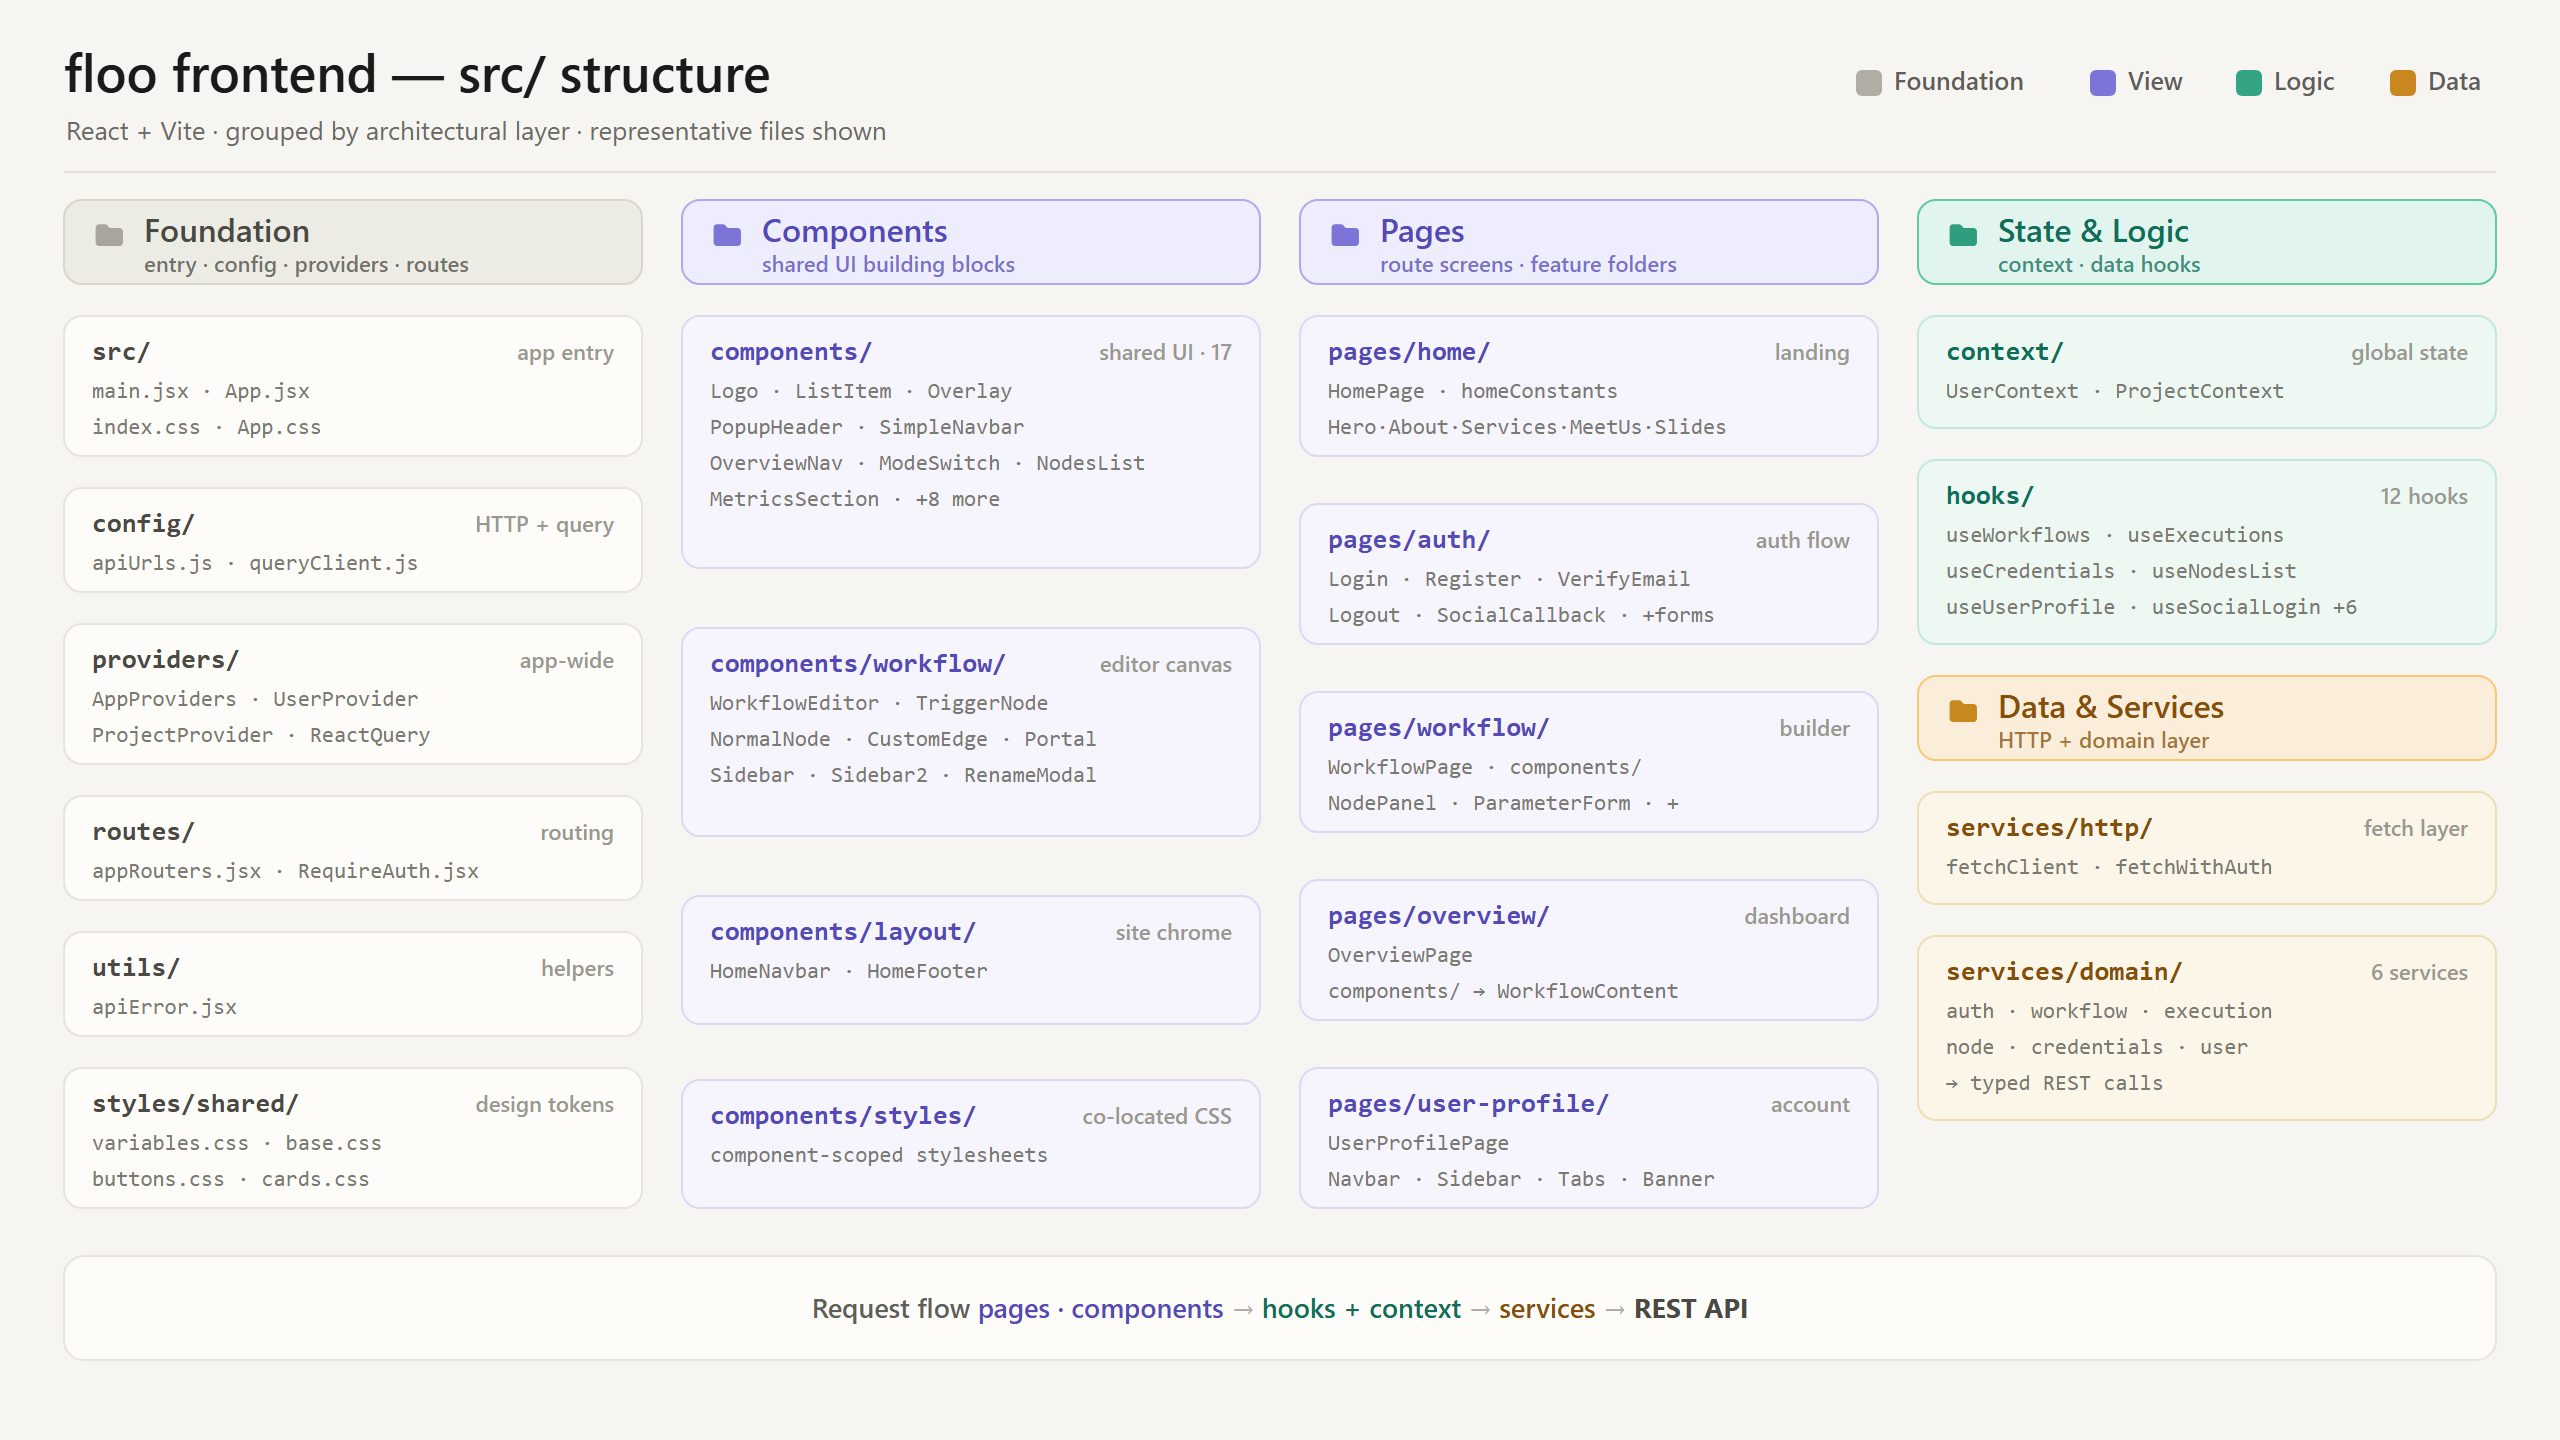
\includegraphics[width=\textwidth]{images/project-structure/project-structure1-image.png}
    \caption{Frontend Architecture and Project Structure Image}
\end{figure}

\subsection{Application Entry Point}

\textbf{Purpose:} Acts as the initial script executed upon application start. It bootstraps the application and hands execution control over to the routing system.

\vspace{0.2cm}
\noindent\textbf{Location:} \texttt{src/main.jsx}

\vspace{0.2cm}
\noindent\textbf{Notes:}
\begin{itemize}
    \item Utilizes React's \texttt{createRoot} to mount the application into the root HTML DOM element.
    \item Injects global stylesheets to establish baseline styling.
    \item Encapsulates the entire component tree within global providers and the router to establish application-wide state.
\end{itemize}

\subsection{Root Component}

\textbf{Purpose:} Serves as the top-level shell component of the application that hosts whichever page the user navigates to.

\vspace{0.2cm}
\noindent\textbf{Location:} \texttt{src/App.jsx}

\vspace{0.2cm}
\noindent\textbf{Notes:}
\begin{itemize}
    \item Renders the router's \texttt{Outlet}, functioning as the dynamic placeholder where the currently active route's page is displayed.
\end{itemize}

\subsection{Global Providers}

\textbf{Purpose:} Supplies application-wide state and services across the entire component tree, mitigating the need for manual "prop drilling" through nested layers.

\vspace{0.2cm}
\noindent\textbf{Location:} \texttt{src/providers/}

\vspace{0.2cm}
\noindent\textbf{Notes:}
\begin{itemize}
    \item Uses an \texttt{AppProviders} wrapper to group all individual providers into a single unified higher-order component.
    \item \textbf{UserProvider:} Manages authentication states and logged-in user data.
    \item \textbf{ProjectProvider:} Tracks the currently selected project workspace.
    \item \textbf{ReactQueryProvider:} Initializes the data-fetching and caching library context.
\end{itemize}

\subsection{Global State Containers}

\textbf{Purpose:} Defines the React Context objects responsible for holding shared application state, acting as the distribution channels filled by providers.

\vspace{0.2cm}
\noindent\textbf{Location:} \texttt{src/context/}

\vspace{0.2cm}
\noindent\textbf{Notes:}
\begin{itemize}
    \item Houses specific contexts such as the User and Project contexts.
    \item Allows any nested component or hook to directly subscribe to and read global values without intermediate propagation.
\end{itemize}

\subsection{Custom Logic Hooks}

\textbf{Purpose:} Abstracts business logic and data-fetching into reusable modules, keeping View components purely presentational and lightweight.

\vspace{0.2cm}
\noindent\textbf{Location:} \texttt{src/hooks/}

\vspace{0.2cm}
\noindent\textbf{Notes:}
\begin{itemize}
    \item Contains highly specialized hooks (e.g., \texttt{useWorkflows}, \texttt{useExecutions}, \texttt{useCredentials}).
    \item Autonomously consumes necessary context (like authentication tokens) and invokes respective API services.
    \item Manages request lifecycles, tracking active loading and error states via React Query to return ready-to-use data to the component.
\end{itemize}

\subsection{API Data Layer}

\textbf{Purpose:} Centralizes all network communication directly with the backend REST API, guaranteeing the rest of the application never interfaces with network requests directly.

\vspace{0.2cm}
\noindent\textbf{Location:} \texttt{src/services/}

\vspace{0.2cm}
\noindent\textbf{Notes:}
\begin{itemize}
    \item Composed of dedicated services (e.g., \texttt{WorkflowService}, \texttt{UserProfileService}) targeting specific REST endpoints.
    \item Utilizes a shared authenticated-fetch helper to automatically append user tokens and process standard JSON responses.
\end{itemize}

\subsection{End-to-End Execution Path}

\textbf{Purpose:} Maps the sequential runtime lifecycle of a user request traveling from the client down to the backend REST API and back.

\begin{figure}[H]
    \centering
    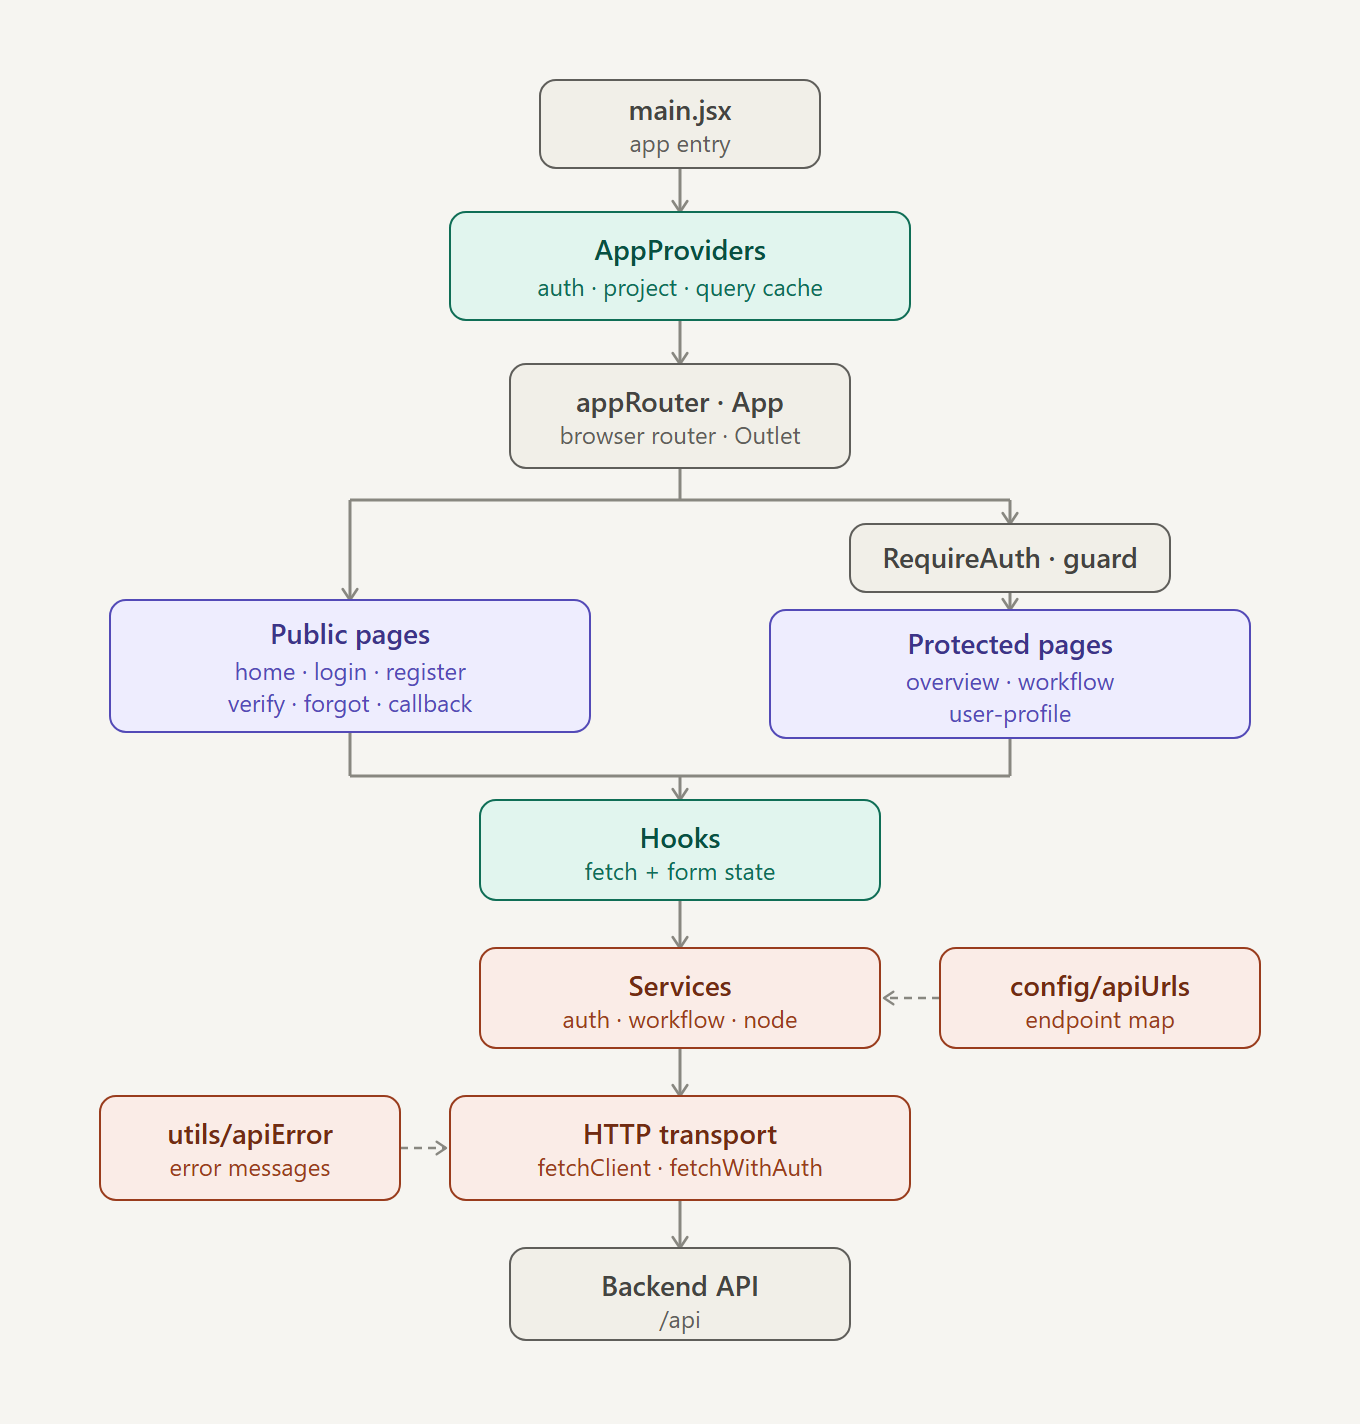
\includegraphics[width=\textwidth]{images/project-structure/project-structure2-image.png}
    \caption{Frontend Architecture and Project Structure Image}
\end{figure}

\vspace{0.2cm}
\noindent\textbf{Execution Sequence:}
\begin{enumerate}
    \item \textbf{Initialization (\texttt{main.jsx}):} The browser loads the app, executes the entry script, creates the React root, and initiates rendering.
    \item \textbf{State Wrapping (\texttt{AppProviders}):} The app is immediately enveloped by providers, guaranteeing universal access to auth state, projects, and the React Query cache.
    \item \textbf{Route Resolution (\texttt{appRouter} \& \texttt{App}):} The router evaluates the URL and injects the corresponding component into the \texttt{App} shell's \texttt{Outlet}.
    \item \textbf{Security Guarding:} Routes are split. Public pages are openly accessible, while protected pages sit behind a \texttt{RequireAuth} interceptor that force-redirects unauthorized traffic to the login screen.
    \item \textbf{Logic Invocation (Hooks):} Page components invoke a custom hook responsible for orchestrating network requests and form states rather than fetching data natively.
    \item \textbf{Service Delegation:} The active hook delegates execution to a targeted service containing the specific backend endpoint mapping.
    \item \textbf{HTTP Transport:} The service dispatches the request through a shared transport utility (\texttt{fetchClient} / \texttt{fetchWithAuth}) to securely attach the session token to the request headers.
    \item \textbf{Backend API Resolution:} The request reaches the backend \texttt{/api} endpoints; the processed response returns up the same exact pipeline to trigger client-side UI state updates.
\end{enumerate}

\vspace{0.2cm}
\noindent\textbf{Supporting Modules:}
\begin{itemize}
    \item \textbf{\texttt{config/apiUrls}:} Supplies the absolute endpoint addresses to the service layer.
    \item \textbf{\texttt{utils/apiError}:} Intercepts failed HTTP responses and translates them into human-readable error messages for the UI hooks to display.
\end{itemize}



\section{AI Workflow Generation Pipeline}
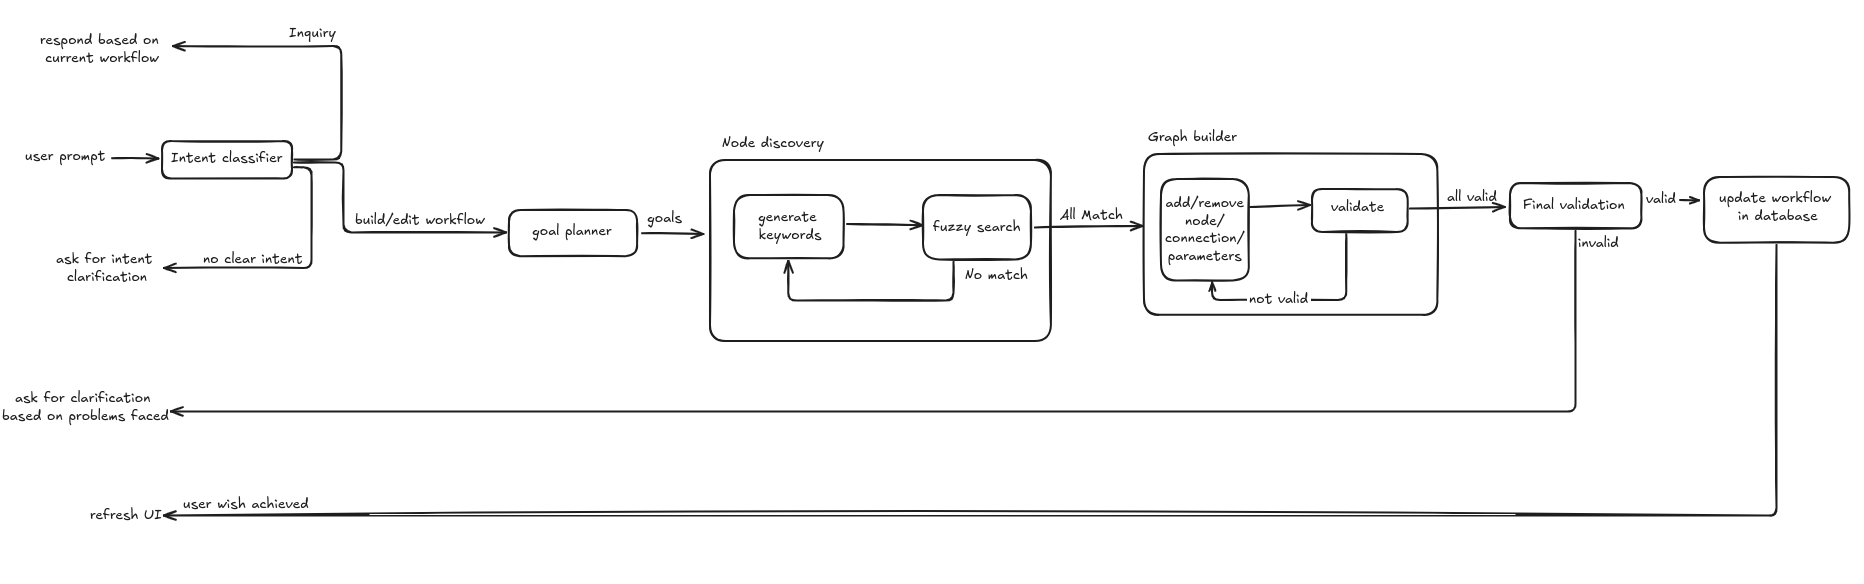
\includegraphics[width=0.85\textwidth]{images/backend/agent.png}

To improve the reliability of AI-generated workflows and reduce the possibility of hallucinated nodes, invalid connections, or incomplete configurations, the workflow generation process is implemented as a multi-agent pipeline. Instead of relying on a single Large Language Model (LLM) to directly generate a workflow, the task is decomposed into several specialized subagents, each responsible for a specific stage of the generation process.

Each subagent is implemented as an independent LLM context with a dedicated system prompt, a defined objective, and a restricted set of available tools. This separation limits the scope of each agent's reasoning process and allows each stage to produce a structured output that can be validated before being passed to the next stage.

The overall pipeline consists of five main stages:

\begin{enumerate}
    \item Intent classification
    \item Workflow planning
    \item Node discovery
    \item Workflow construction
    \item Workflow validation
\end{enumerate}

Each stage progressively transforms the user's natural language request into a valid executable workflow.

\subsection{Intent Classifier}

The Intent Classifier is the entry point of the AI workflow generation pipeline. Its responsibility is to determine the user's objective and select the appropriate processing path.

The classifier analyzes the user prompt and categorizes it into one of three supported intents:

\begin{itemize}
    \item \textbf{Inquiry}: The user requests information about the current workflow, available nodes, or system capabilities. The agent responds by providing the required information without modifying the workflow.
    
    \item \textbf{Build}: The user requests the creation of a new workflow. The request is forwarded to the planning stage to generate a workflow specification.
    
    \item \textbf{Edit}: The user requests modifications to an existing workflow. The existing workflow context is provided to later stages so that the required changes can be applied.
\end{itemize}

The classifier is intentionally isolated from workflow generation tools since its role is only understanding the user's intention. If the intent cannot be determined with sufficient confidence, the agent requests additional clarification rather than making assumptions.

\subsection{Planner}

The Planner converts the high-level user request into a structured sequence of implementation goals. Since user descriptions are usually expressed in terms of desired outcomes rather than specific workflow components, the planner acts as an intermediate reasoning layer between user intent and workflow implementation.

Each generated goal describes a single logical operation required to achieve the final objective. A goal contains:

\begin{itemize}
    \item A description of the required operation.
    \item Search keywords describing the expected functionality.
    \item The expected input and output behavior when applicable.
\end{itemize}

For example, a request such as "resize uploaded images and notify me when finished" can be decomposed into multiple goals including image processing, file handling, and notification delivery.

This decomposition enables the following stages to operate on smaller, well-defined tasks instead of attempting to solve the entire workflow generation problem at once.

\subsection{Node Discoverer}

The Node Discoverer is responsible for mapping planning goals into available workflow nodes from the node registry.

Since the LLM does not directly know the complete list of available nodes, the discoverer interacts with the node registry through search tools. It performs semantic discovery using fuzzy matching techniques over node names and descriptions.

The discovery process follows an iterative approach:

\begin{enumerate}
    \item Extract search terms from the planning goal.
    \item Query the node registry using fuzzy search.
    \item Evaluate the returned candidate nodes.
    \item Refine the search terms if no suitable node is found.
    \item Repeat until a suitable node is selected or the retry limit is reached.
\end{enumerate}

The output of this stage is a collection of selected nodes that can be used to implement each planning goal.

Restricting node selection to the registry prevents the model from generating nonexistent components and ensures that all produced workflows are compatible with the execution engine.

\subsection{Workflow Construction}

After identifying the required nodes, the Workflow Construction stage is responsible for assembling the final workflow graph.

During this stage, the LLM is provided with a controlled set of workflow manipulation tools. These tools allow the agent to perform operations such as:

\begin{itemize}
    \item Adding nodes to the workflow graph.
    \item Removing unnecessary nodes.
    \item Creating connections between node inputs and outputs.
    \item Updating node parameters and configurations.
    \item Inspecting the current workflow state.
\end{itemize}

The construction process follows a tool-based iterative loop. Instead of generating the complete workflow structure in a single response, the agent repeatedly analyzes the current graph state and invokes the required tools until the workflow satisfies the planned objectives.

This approach provides several advantages:

\begin{itemize}
    \item Prevents invalid graph structures caused by single-pass generation.
    \item Allows the model to react to tool results.
    \item Enables incremental correction during construction.
    \item Keeps workflow modifications explicit and traceable.
\end{itemize}

The final output of this stage is a complete workflow graph containing nodes, connections, and configured parameters.

\subsection{Validator}

The Validator is the final stage of the pipeline and is responsible for ensuring that the generated workflow is executable and consistent.

The validator performs multiple checks, including:

\begin{itemize}
    \item Verifying that all referenced nodes exist in the node registry.
    \item Checking that required parameters are provided.
    \item Ensuring that node connections are compatible.
    \item Detecting disconnected or unreachable nodes.
    \item Validating the overall workflow structure.
\end{itemize}

If the validator identifies problems that can be automatically corrected, it applies the necessary fixes. For example, missing default parameters or incorrect connections may be repaired automatically.

For issues requiring additional information from the user, such as missing credentials or ambiguous configuration values, the validator reports the problem and requests clarification before the workflow is stored.

\subsection{Agent Tool Isolation}

A key design principle of the pipeline is restricting each subagent to only the tools required for its responsibility. This prevents unintended modifications and reduces the possibility of invalid reasoning.

For example:

\begin{itemize}
    \item The Intent Classifier has no workflow modification tools.
    \item The Planner only produces workflow specifications.
    \item The Node Discoverer only accesses node search capabilities.
    \item The Construction Agent receives workflow editing tools.
    \item The Validator receives workflow inspection and repair tools.
\end{itemize}

This modular architecture improves reliability, simplifies debugging, and allows individual stages to be independently improved without affecting the rest of the system.

\section{AI Models Integration}

\subsection{Overview}

To extend the workflow engine with intelligent image-processing capabilities, an AI integration layer was introduced. The AI team developed multiple computer vision models in Python, including image processing and analysis tasks such as edge detection, optical character recognition (OCR), image classification, and image cropping.

Since the workflow engine is implemented in Node.js while the AI models are implemented in Python, a communication mechanism was required to allow both systems to work together without introducing tight coupling.

To achieve this, the AI models were exposed as RESTful services using \textbf{FastAPI}, allowing the workflow engine to invoke AI functionality through standard HTTP requests.


\subsection{Architecture}

The integration follows a service-oriented architecture where the workflow engine communicates with an independent AI service.

The backend is responsible for workflow orchestration, while the FastAPI service is responsible for executing AI models and managing generated outputs.

This separation allows both systems to evolve independently while maintaining a clean interface between them.


\subsection{AI Nodes}

Each AI capability is represented as a workflow node.

Instead of embedding image-processing algorithms directly inside the backend, every AI node acts as an adapter between the workflow engine and the corresponding AI model.

Examples of implemented AI nodes include:

\begin{itemize}
    \item Edge Detection
    \item OCR
    \item Image Classification
    \item Image Cropping
\end{itemize}

All AI nodes inherit from the common \texttt{Node} base class and therefore integrate seamlessly with the execution engine.

During execution, the node performs the following steps:

\begin{enumerate}
    \item Retrieves execution context and node parameters.
    \item Reads the required execution metadata.
    \item Sends an HTTP request to the FastAPI service.
    \item Waits for the processing result.
    \item Stores the returned output information.
    \item Passes the output to downstream workflow nodes.
\end{enumerate}

This design enables AI operations to behave exactly like any other workflow node while hiding the implementation details of the underlying models.


\subsection{Metadata-Based Communication}

Rather than sending only the image to the AI service, the backend also sends execution metadata, including:

\begin{itemize}
    \item User ID
    \item Project ID
    \item Execution ID
    \item Node ID
\end{itemize}

This metadata enables the AI service to correctly associate generated outputs with the corresponding workflow execution.

It also allows generated files to be organized automatically according to the workflow structure without requiring additional backend processing.


\subsection{Optimized Output Handling}

One of the architectural decisions made during the AI integration was to avoid transferring processed images back to the backend.

Instead of following the traditional workflow:

\begin{verbatim}
Python Model
      |
      v
Node.js Backend
      |
      v
Cloud Storage
\end{verbatim}

the implemented architecture performs the upload directly from the FastAPI service:

\begin{verbatim}
Python Model
      |
      v
FastAPI Service
      |
      v
Upload Result
      |
      v
Cloud Storage
      |
      v
Return Output URL
      |
      v
Node.js Backend
\end{verbatim}

Only the generated image URL is returned to the backend.

This approach provides several advantages:

\begin{itemize}
    \item Reduced network traffic
    \item Lower memory consumption
    \item Faster workflow execution
    \item Elimination of redundant file transfers
    \item Clear separation of responsibilities
\end{itemize}


\subsection{Design Benefits}

The adopted architecture provides several software engineering advantages:

\begin{itemize}
    \item \textbf{Loose Coupling:} The backend is independent of the internal implementation of AI models.
    
    \item \textbf{Modularity:} AI models can be updated or replaced without modifying the workflow engine.
    
    \item \textbf{Scalability:} Additional AI services can be integrated by exposing new REST endpoints.
    
    \item \textbf{Reusability:} Every AI capability is encapsulated as a reusable workflow node.
    
    \item \textbf{Maintainability:} The AI service and workflow engine can be developed and deployed independently.
\end{itemize}